\documentclass[12pt,a4paper,oneside]{memoir}

% ===============================
% 1. PACKAGES
% ===============================
\usepackage{times}
\usepackage[T1]{fontenc}
\usepackage{xcolor}
\usepackage{graphicx}
\usepackage{amsmath,amssymb}
\usepackage{booktabs}
\usepackage{hyperref}
\usepackage{caption}
\usepackage[backend=biber,style=ieee]{biblatex}
\usepackage{siunitx}
\usepackage{array}
\usepackage{longtable}
\usepackage{placeins}
\usepackage{pdflscape}
\usepackage{lipsum}        % dummy text
\usepackage[linesnumbered,ruled,vlined]{algorithm2e}
\usepackage{float}
%
\usepackage{listings}
% --- Custom Colors for Python Beautification ---
\definecolor{codegreen}{rgb}{0,0.6,0}
\definecolor{codegray}{rgb}{0.5,0.5,0.5}
\definecolor{codepurple}{rgb}{0.58,0,0.82}
\definecolor{backcolour}{rgb}{0.96,0.96,0.97}
\definecolor{codeblue}{rgb}{0.1,0.2,0.8}
% --- Global Listings Style ---
\lstset{
	backgroundcolor=\color{backcolour},   
	commentstyle=\color{codegreen},
	keywordstyle=\color{codeblue}\bfseries,
	numberstyle=\tiny\color{codegray},
	stringstyle=\color{codepurple},
	basicstyle=\ttfamily\scriptsize,
	breakatwhitespace=false,         
	breaklines=true,                 
	captionpos=b,                    
	keepspaces=true,                 
	numbers=left,                    
	numbersep=8pt,                  
	showspaces=false,                
	showstringspaces=false,
	showtabs=false,                  
	tabsize=1,
	frame=single,
	rulecolor=\color{codegray!30},
	language=Python
}

% ===============================
% 2. BIBLIOGRAPHY SETUP
% ===============================
\addbibresource{References.bib}

% ===============================
% 3. COLORS & SPACING
% ===============================
\definecolor{deepred}{RGB}{152,50,34}
\newcommand{\earlierrevision}[1]{\textcolor{blue}{#1}}
\newcommand{\newrevision}[1]{\textcolor{green!45!black}{#1}}
\linespread{1.25}
\setlength{\parindent}{0pt}
\setlength{\parskip}{6pt}
\hyphenpenalty=10000
\exhyphenpenalty=10000
\emergencystretch=3em

% ===============================
% 4. PAGE LAYOUT
% ===============================
\setlrmarginsandblock{1.1in}{1.1in}{*}
\setulmarginsandblock{1in}{1in}{*}
\checkandfixthelayout
\pagestyle{plain}

% ===============================
% 5. NUMBERING & TOC DEPTH
% ===============================
\setsecnumdepth{subsubsection}
\maxsecnumdepth{subsubsection}
\settocdepth{subsection}
\setcounter{tocdepth}{2}

% ===============================
% 6. CHAPTER STYLE (Centered & ALL CAPS)
% ===============================
\makechapterstyle{sdpstyle}{
	\renewcommand{\printchaptername}{}
	\renewcommand{\chapternamenum}{}
	\renewcommand{\printchapternum}{\centering\large\bfseries \thechapter.\space}
	\renewcommand{\chaptitlefont}{\large\bfseries\centering}
	\renewcommand{\afterchapternum}{}
	\renewcommand{\printchaptertitle}[1]{%
		\chaptitlefont\MakeUppercase{##1}%
	}
}
\chapterstyle{sdpstyle}

% ===============================
% 7. HEADING STYLES
% ===============================
\hypersetup{
	colorlinks=false,
	linkcolor=black,
	citecolor=black,
	filecolor=black,
	urlcolor=black,
	linktoc=all,
	pdfborder={0 0 0},
}
\setsecheadstyle{\color{black}\normalsize\bfseries\scshape}
\setsubsecheadstyle{\color{black}\normalsize\bfseries\scshape}
\setsubsubsecheadstyle{\color{black}\bfseries\normalshape}
\renewcommand{\thesubsubsection}{\textcolor{black}{\thesubsection.\arabic{subsubsection}}}

% --- Paragraph heading style (memoir native) ---
\setparaheadstyle{\bfseries}
\setafterparaskip{1.5ex plus .4ex minus .2ex}
\setbeforeparaskip{3.25ex plus 1ex minus .2ex}

% ===============================
% 8. TOC STYLING
% ===============================
\renewcommand{\printtoctitle}[1]{\centering\large\bfseries \MakeUppercase{#1}}
\renewcommand{\cftchapterfont}{\scshape\bfseries\color{black}}
\renewcommand{\cftchapterpagefont}{\color{black}}
\renewcommand{\cftsectionfont}{\scshape\color{black}}
\renewcommand{\cftsectionpagefont}{\color{black}}
\renewcommand{\cftsubsectionfont}{\normalshape\color{black}}
\renewcommand{\cftsubsectionpagefont}{\color{black}}

% ===============================
% 9. UNNUMBERED RED HEADING COMMAND
% ===============================
\newcommand{\redheading}[1]{%
	\vspace{6pt}
	{\color{black}\bfseries\normalshape #1}\par
	\noindent
	\vspace{0pt}%
}

% ===============================
% 10. FIGURE & TABLE CAPTIONS
% ===============================
\captionnamefont{\scshape}
\captiontitlefont{\upshape}
\captiondelim{.\ }
\setlength{\belowcaptionskip}{10pt}
\setlength{\abovecaptionskip}{10pt}

% ===============================
% 11. CONTENTS NAME
% ===============================
\renewcommand{\contentsname}{CONTENTS}

% ===============================
% 12. ALGORITHMS (algorithm2e)
% ===============================
\renewcommand{\listalgorithmcfname}{List of Algorithms}

% ===============================
% 13. PAGE NUMBERING & LIST STYLING
% ===============================
\frontmatter
\pagenumbering{roman}

% --- Figure Spacing (Tightened) ---
\renewcommand{\cftfigurename}{Figure~}
\renewcommand{\cftfigureaftersnum}{.}
\setlength{\cftfigurenumwidth}{3.0em} 
\setlength{\cftfigureindent}{0em}    

% --- Table Spacing (Tightened) ---
\renewcommand{\cfttablename}{Table~}
\renewcommand{\cfttableaftersnum}{.}
\setlength{\cfttablenumwidth}{3.0em} 
\setlength{\cfttableindent}{0em}    

% --- Algorithm List Styling ---
\makeatletter
% Force "Algorithm" prefix into the list
\let\oldl@algocf\l@algocf
\renewcommand{\l@algocf}[2]{\oldl@algocf{Algorithm #1}{#2}}

% Direct memoir-style length setting for Algorithms
\AtBeginDocument{
	\newlength{\cftalgocfnumwidth}
	\setlength{\cftalgocfnumwidth}{6em}
	\newlength{\cftalgocfindent}
	\setlength{\cftalgocfindent}{0em}
}
\makeatother

% ===============================
% 14. APPENDIX SETUP 
% ===============================
\makeatletter
\g@addto@macro\appendix{%
	% 1. Force A, B, C numbering
	\renewcommand{\thechapter}{\Alph{chapter}}
	
	% 2. Fix the Header on the actual page
	\renewcommand{\printchapternum}{%
		\centering\large\bfseries APPENDIX \thechapter.\space%
	}
	
	% 3. Override the chapter command
	\def\chapter{\@ifstar{\@schapter}{\@dblarg\@manualappendixchapter}}
}

\def\@manualappendixchapter[#1]#2{%
	\cleardoublepage % <--- THIS FORCES THE NEW PAGE
	\refstepcounter{chapter}%
	% Writes "Appendix A. Title" to the TOC
	\addcontentsline{toc}{chapter}{\scshape Appendix \thechapter.\hspace{1em}#1}%
	\chaptermark{#1}%
	\if@twocolumn
	\@topnewpage[\@makechapterhead{#2}]%
	\else
	\@makechapterhead{#2}%
	\@afterheading
	\fi
}
\makeatother
%
% ==================================================
% DOCUMENT START
% ==================================================
\begin{document}

% --- TITLE PAGE ---
\begin{titlingpage}
	\centering
	\linespread{1.0}
	\vspace*{0.5in}
	{\large\textbf{\MakeUppercase{Design and Implementation of a Scalable IoT-Based Acoustic Detection System for Early Red Palm Weevil Infestation}}\par}
	\vspace{0.7in}
	{\large\textbf{\textsc{CMP/COE490: Senior Design Project}}\par}
	\vspace{0.4in}
	Submitted in Partial Fulfillment of the\\
	Requirements for the Degree of\\
	\vspace{0.4in}
	\textbf{\textsc{Bachelor of Science in Computer Science and Engineering}}
	\vspace{0.4in}

	by

	\vspace{0.2in}

	\begin{tabular}{p{2.2in} r}
		Khalid Hamdan         & 99009  \\
		Abdurrahman Maricar   & 96961  \\
		Kareem Mahmoud        & 97349  \\
		Haitham Ayyash        & 103430 \\
	\end{tabular}

	\vspace{0.4in}

	\textit{Advisors}\\[0.15in]
	Dr.\ Mohamed Alhajri\\
	Dr.\ Taha Landolsi

	\vfill

	\makebox[\textwidth][c]{%
		
\includegraphics[width=0.175\textwidth]{AUSlogo.png}
	}

	\vspace{0.1in}

	Department of Computer Science and Engineering\\
	American University of Sharjah\\[0.15in]
	Spring 2026
\end{titlingpage}

% --- ACKNOWLEDGMENTS ---
\chapter*{Acknowledgments}
\thispagestyle{plain}
\addcontentsline{toc}{chapter}{Acknowledgments}
\vspace*{0.4in}
\begin{center}
\itshape
With sincere gratitude
\end{center}
\vspace{0.2in}
\begin{center}
On behalf of our Senior Design team, we would like to extend our sincere thanks to our advisor, Dr.\ Mohamed Alhajri, and our co-advisor, Dr.\ Taha Landolsi, for their guidance, dedication, and continuous support throughout this project.

We are also grateful to the American University of Sharjah and the College of Engineering for providing us with the opportunity and support to pursue this work.

Last but not least, we would like to express our heartfelt thanks to our families for their constant encouragement, patience, and unwavering support.
\end{center}

\vspace{0.5in}
\begin{flushright}
\textit{Respectfully submitted,}\\[0.1in]
\textbf{The Senior Design Team}
\end{flushright}
\clearpage

% --- ABSTRACT ---

\chapter*{Abstract}
\thispagestyle{plain}
\addcontentsline{toc}{chapter}{Abstract}
Palms face significant threats from the Red Palm Weevil (RPW), making RPW management challenging due to the internal development of larvae within the trunk, which often go unnoticed until infestations escalate. This paper presents an innovative, scalable Internet of Things (IoT) system for the acoustic detection and early identification of RPW. The proposed system is designed to use low-cost, trunk-mounted piezoelectric sensors to capture vibrations caused by larval activity within the palm. These sensors are based on ESP32 microcontrollers and LoRa communication modules and are intended to form a wireless sensor network that transmits data packets to a central hub for cloud storage, analysis, and alert generation.

\earlierrevision{To support reliable detection, the proposed design applies bandpass filtering, SNR gating, and MFCC extraction before deep learning inference. A web dashboard is planned to show node health, scheduled measurements, and potential infestation alerts. The modular architecture is intended to support later expansion after prototype and field validation. By providing earlier screening information, the minimally invasive system may help managers target inspections and treatment, but pesticide, economic, and large-scale benefits must be measured rather than assumed.}

\clearpage

% --- CONTENTS (The TOC itself) ---
\tableofcontents* \clearpage

% --- LIST OF FIGURES ---
\listoffigures
\clearpage

% --- LIST OF TABLES ---
\listoftables
\clearpage

% --- GLOSSARY ---

\chapter*{Glossary}
\thispagestyle{plain}
\addcontentsline{toc}{chapter}{Glossary}
\renewcommand{\arraystretch}{1.3}
\begin{tabular}{@{}p{0.12\linewidth} p{0.85\linewidth}@{}}
	\textbf{ADC} & Analog-to-Digital Converter \\
	\textbf{AI} & Artificial Intelligence \\
	\textbf{ANN} & Artificial Neural Network \\
	\textbf{API} & Application Programming Interface \\
	\textbf{Bi-LSTM} & Bidirectional Long Short-Term Memory \\
	\textbf{CNN} & Convolutional Neural Network \\
	\textbf{DAS} & Distributed Acoustic Sensing \\
	\textbf{ESP32} & Espressif 32-bit Microcontroller \\
	\textbf{IoT} & Internet of Things \\
	\textbf{IPM} & Integrated Pest Management \\
	\textbf{JSON} & Java Script Object Notation \\
	\textbf{JWT} & JSON Web Token \\
	\textbf{LoRa} & Long Range Radio \\
	\textbf{ML} & Machine Learning \\
	\textbf{RPW} & Red Palm Weevil \\
	\textbf{SNR} & Signal-to-Noise Ratio \\
	\textbf{UI} & User Interface \\
	\textbf{VOC} & Volatile Organic Compound \\
	\textbf{Wi-Fi} & Wireless Fidelity \\
	\textbf{WSN} & Wireless Sensor Network \\
	\textbf{$\Phi$-OTDR} & Phase-Sensitive Optical Time-Domain Reflectometry \\
\end{tabular}

\clearpage

\mainmatter
\pagenumbering{arabic}

\chapter{Introduction}
\label{ch:Introduction}
 
% ===============================
% CHAPTER 1: INTRODUCTION
% ===============================
 
\section{Motivation}
\label{sec:Motivation}
 
The driving force behind this project is the increasing effect of Red Palm Weevil (RPW) infestations on agriculture and the economy. This section assesses the current state of the RPW infestation and evaluates the existing detection technologies.
 
\subsection{Current Situation of Red Palm Weevil Infestation}
 
The RPW (Rhynchophorus ferrugineus) is currently recognized as one of the most destructive and invasive pests threatening palm species worldwide, especially in the Middle East, North Africa, and the Mediterranean basin. The economic losses associated with severely infested palms in Gulf countries have been estimated in the millions of U.S. dollars annually \cite{saleem2022,alaufi2026}. The primary challenge lies in the ``hidden'' nature of the pest. For most of the larval life cycle, it remains concealed inside the trunk while feeding, making visual inspection unreliable until the damage is already advanced \cite{saleem2022,alaufi2026}. Visible symptoms such as holes in the trunk or crown, oozing brown viscous liquid, and collapsed crowns usually indicate a severe infestation that has progressed to the point where the palm tree is already dying and difficult or impossible to save \cite{saleem2022,alaufi2026}. These limitations motivate the development of a cost-effective, reliable, and non-invasive early detection system capable of deployment across large plantations.
 
\begin{figure}[H]
\centering
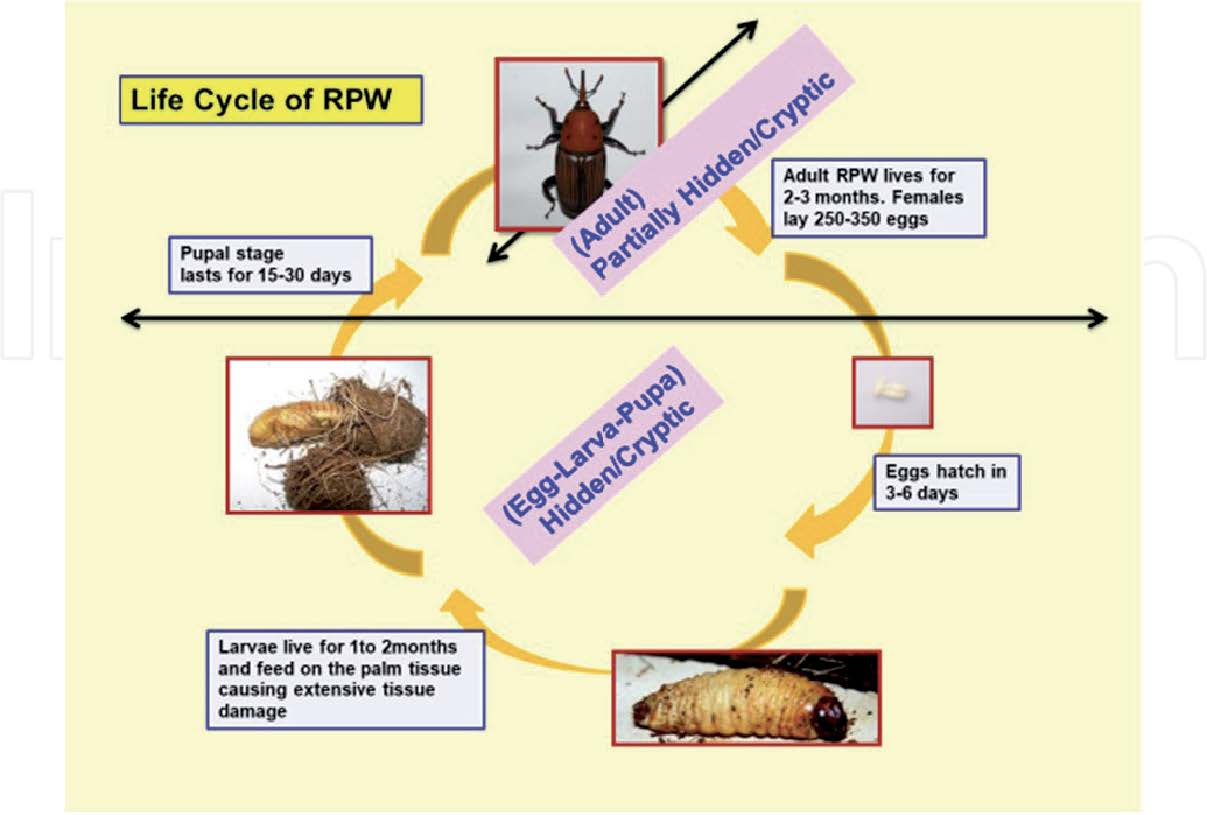
\includegraphics[width=0.75\textwidth]{figures/fig1_rpw_lifecycle.jpeg}
\caption{Schematic Diagram Depicting the Life Cycle of RPW \cite{alaufi2026}}
\label{fig:rpw_lifecycle}
\end{figure}
 
\begin{figure}[H]
\centering
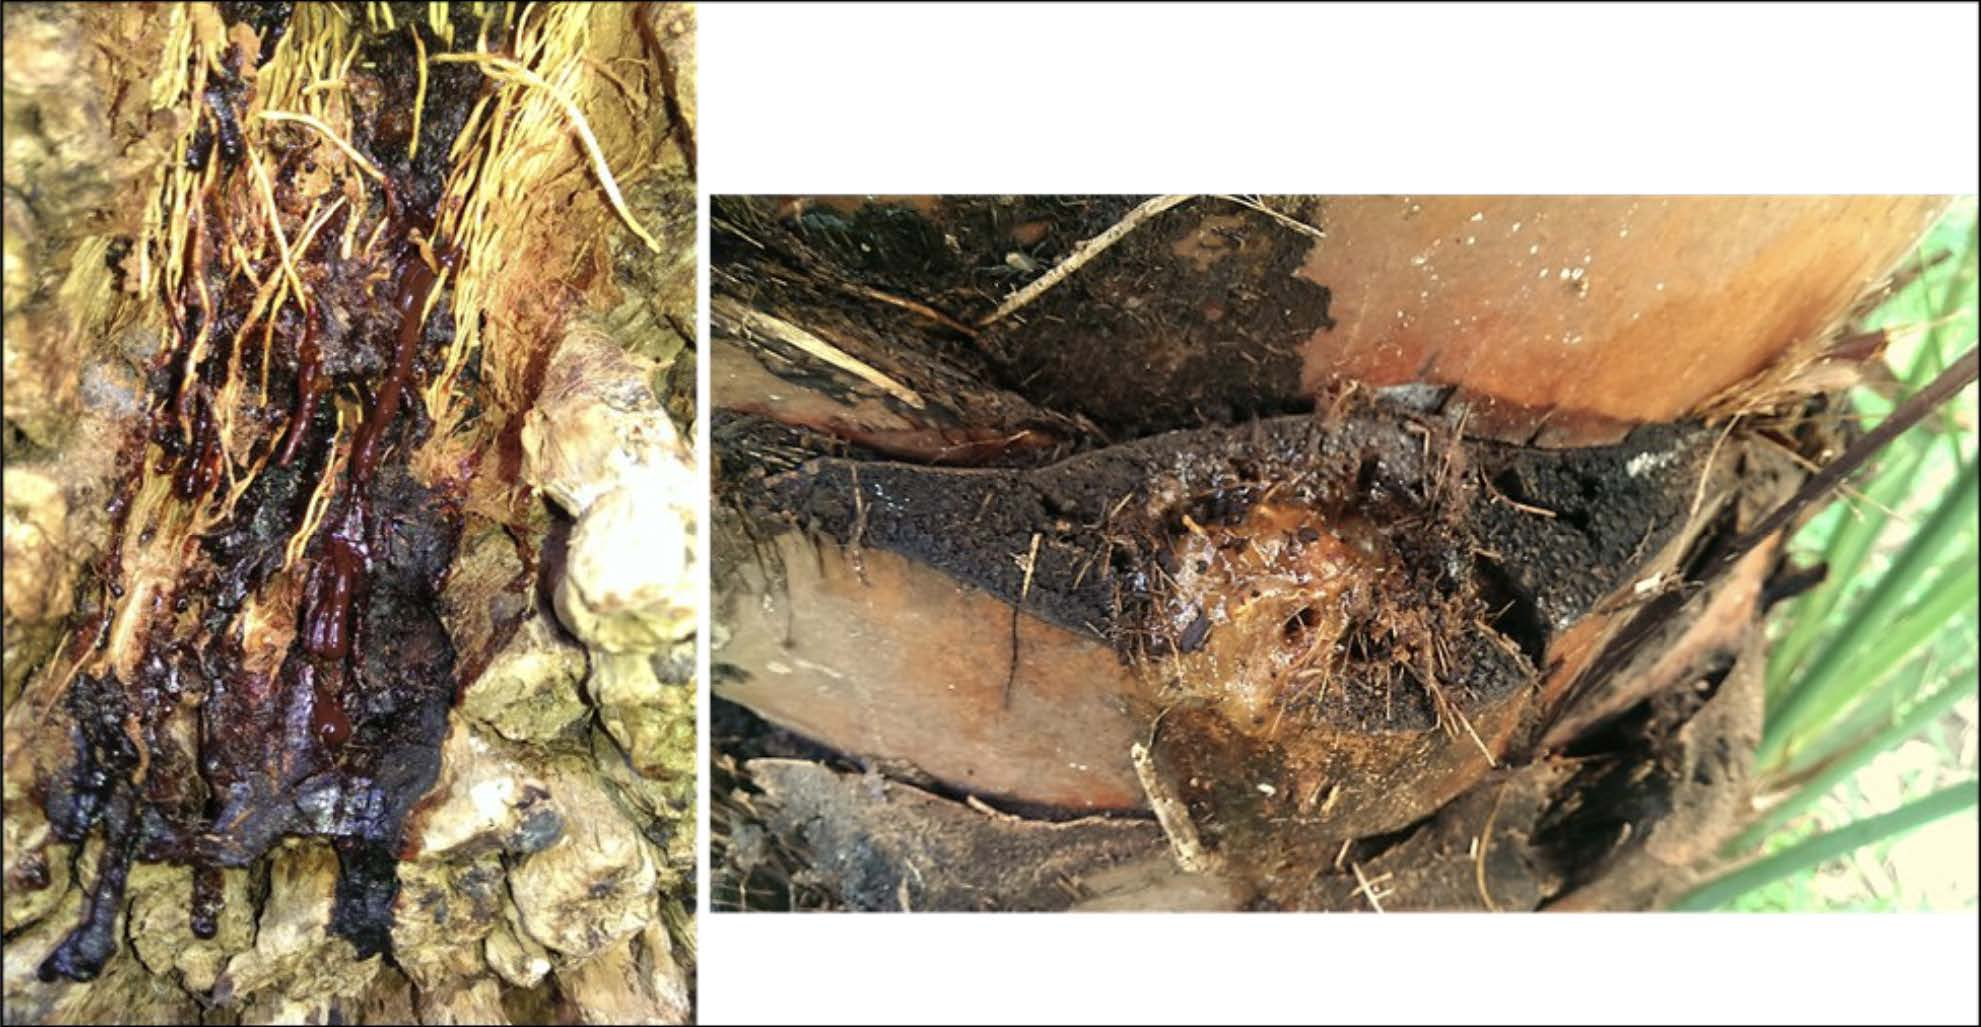
\includegraphics[width=0.75\textwidth]{figures/fig2_viscous_fluid.jpeg}
\caption{Viscous fluids ooze from the tunnels due to larvae inside the palm tree \cite{alaufi2026}}
\label{fig:viscous_fluid}
\end{figure}

\FloatBarrier
 
\subsection{Existing Solutions and Their Limitations}
 
Several methods have been explored to tackle the early detection of the RPW infestations, yet most existing approaches suffer from limitations related to scalability, invasiveness, cost, or detection accuracy. Visual and manual inspection remain the most adopted techniques; however, it is labor intensive, expensive, and subjective to the skills of the laborer. Even trained experts can inspect only a limited number of trees per day, and this method is particularly ineffective for detecting early-stage infestations due to the concealed larval activity inside the trunk \cite{saleem2022,alaufi2026}.
 
\begin{figure}[H]
\centering
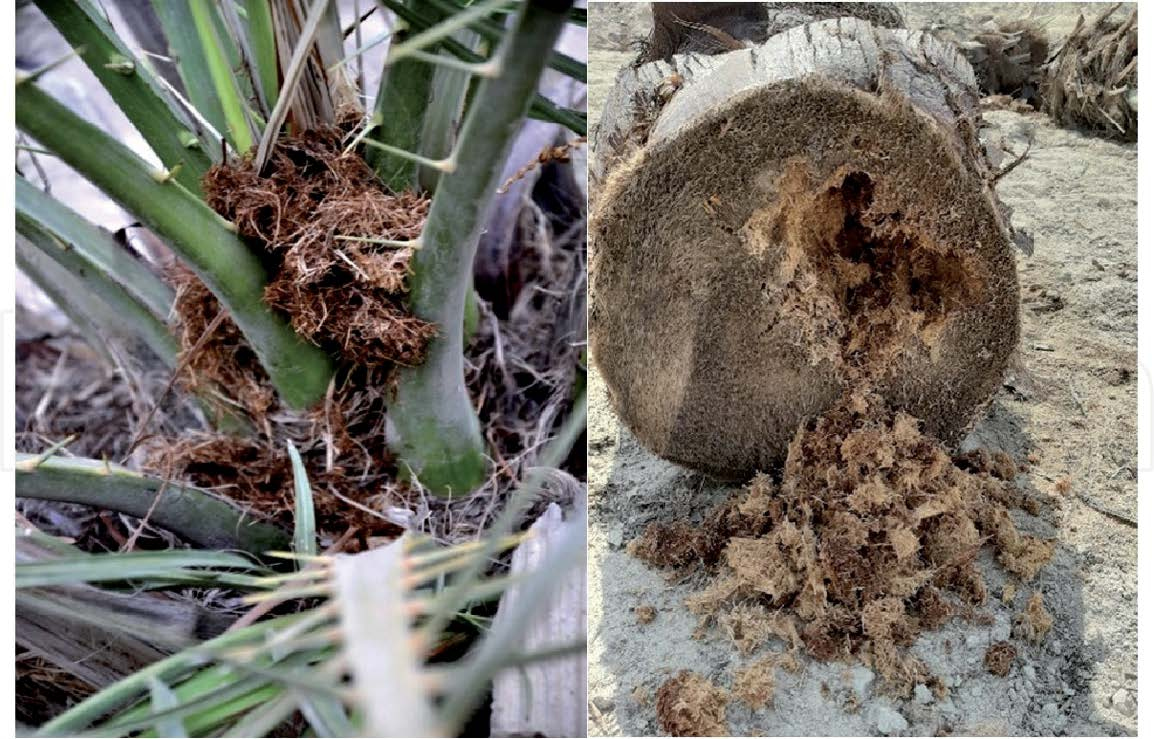
\includegraphics[width=0.75\textwidth]{figures/fig3_infected_crown.jpeg}
\caption{The crown of an infested young date palm (left) ejects chewed-up fibers. Internal palm tissue
shattered because of RPW Larvae consumption \cite{alaufi2026}}
\label{fig:infested_crown}
\end{figure}
 
Another standard method is to use pheromone trapping, which provides valuable information on adult weevil population trends and overall infestation pressure \cite{shukla2018,na2024}. However, traps only work on adult insects and yield no information about actual larval activity occurring inside the palm trees \cite{saleem2022}. Likewise, thermal imaging and remote sensing methods attempt to measure physiological stress signals or internal heat signatures, but these systems are frequently influenced by environmental conditions and generally provide lower reliability for large-scale field assessment than acoustic methods \cite{saleem2022,alaufi2026}. Conventional acoustic sensors are therefore a more promising early-warning approach \cite{karar2021,karar2022}. Piezoelectric probe-based devices are highly sensitive to larval gnawing sounds and, under controlled conditions, may detect infestations within the first two weeks of larval development \cite{ashry2020,ashry2022cnn}. Although such systems are typically invasive (e.g., they involve drilling the tree trunk) \cite{pinhas2008,karar2022}, they provide reliable and well-established detection performance. Despite their higher installation and maintenance costs, they remain suitable for targeted monitoring in semi-controlled environments \cite{karar2022}.

\begin{figure}[H]
\centering
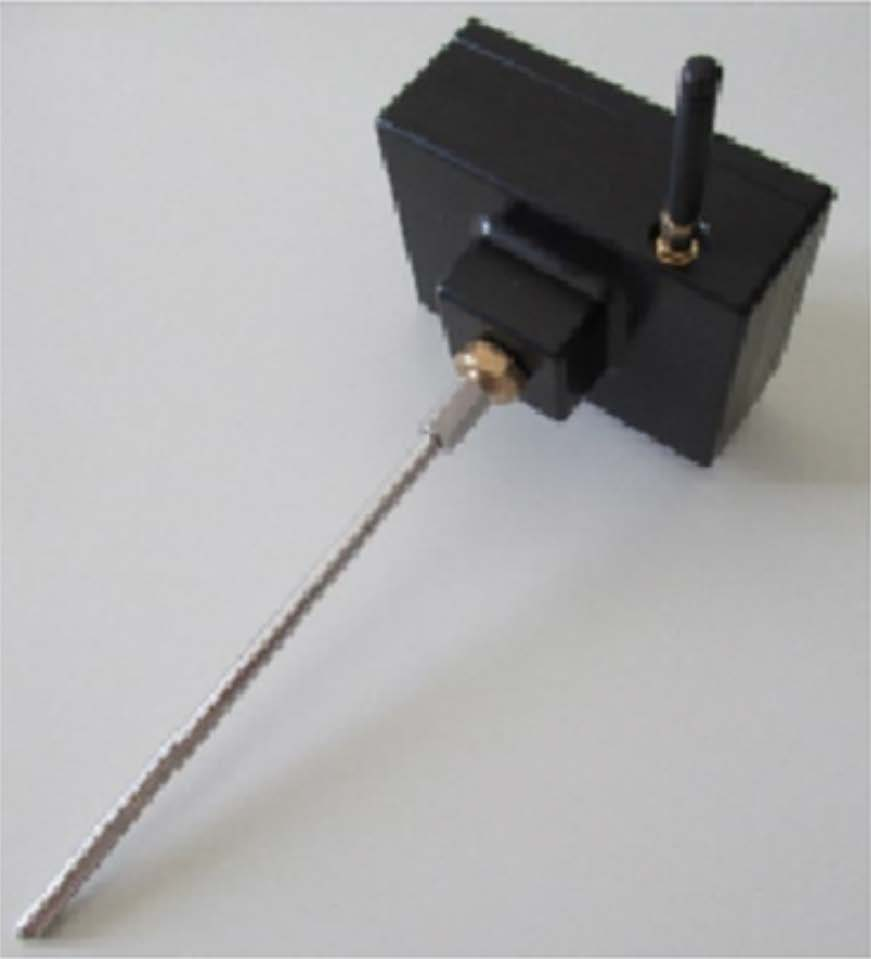
\includegraphics[width=0.5\textwidth]{figures/fig4_treevibes.jpeg}
\caption{TreeVibes sensing device for acquiring sounds of RPW larvae \cite{rigakis2021}}
\label{fig:treevibes}
\end{figure}
 
On the other hand, the combination of Distributed Acoustic Sensing (DAS) and Convolutional Neural Networks (CNNs) is the path with higher potential to meet project goals \cite{ashry2020,wang2021,ashry2022cnn}. DAS technology turns a conventional optical fiber into an external vibration sensor, allowing a single cable wrapped non-invasively around trunks to monitor many trees concurrently \cite{ashry2020,mao2021}. In conjunction with CNN-based classifiers, this method has reported classification accuracies between about 97\% and 99.9\% under controlled and semi-controlled studies \cite{wang2021,ashry2022cnn}. However, due to the high cost for installation, the focus will be on the implementation and evaluation of the conventional acoustic sensing approach as a practical and experimental solution.
 
 
 
\section{Project Description}
\label{sec:Description}
 
\earlierrevision{While DAS represents the highest-performing solution in the literature, its installation cost renders it impractical for large-scale deployment. This project aims to develop an affordable, IoT-based acoustic detection system for larvae (of RPW) in an early infestation stage. Instead of expensive distributed fiber-optic technology, the new system will be made from arrays of low-cost piezoelectric contact sensors mechanically coupled to palm trunks, capable of detecting internal vibrations produced by larval feeding and movement. By combining low-cost sensor devices, deep learning classifiers and cloud-based data analytics, this work intends to investigate a scalable and affordable open solution for real-time plantation monitoring at large-scale agroecological landscapes. The architecture follows a three-tier design: trunk-mounted piezoelectric sensing nodes transmit compact feature packets via LoRa to a cluster head, which aggregates and forwards data to a cloud backend for deep learning classification. The proposed system is intended to support earlier screening than visual inspection, subject to prototype and field validation \cite{ashry2020,ashry2022cnn,karar2022}. The system is designed around low-cost components, a modular IoT infrastructure, and automated analysis tools, to be low-cost and widely deployed. Thus, continuous remote monitoring could help reduce the considerable amount of field labor involved in pest control, and supply information to help reduce pesticide use, both of which would be helpful economically and environmentally \cite{saleem2022,karar2022}. As a secondary contribution, this project evaluates the recently introduced Mamba selective state-space model architecture for RPW acoustic classification, comparing it against established CNN and CNN-LSTM baselines.}

\newrevision{The baseline packet format is a design starting point, not a LoRa capacity claim. The project will compare it with smaller, versioned binary packets and report the measured payload size and airtime under the selected regional radio settings.}
 
\section{Problem Statement}
\label{sec:Statement}
 
\earlierrevision{Red Palm Weevil (RPW) is a destructive pest of palm species, particularly date palms in the Middle East and North Africa. Its larvae feed inside the trunk, where visual inspection cannot reliably detect early activity. When external symptoms such as holes, oozing sap, or crown collapse appear, internal damage may already be severe and treatment may be less effective \cite{saleem2022,ashry2022cnn}. This delay between infestation and visible detection can increase tree loss, treatment costs, and unnecessary pesticide use.}
 
\earlierrevision{This project addresses that gap by designing and validating a low-cost IoT system that monitors trunk vibrations produced by larval feeding and movement. Trunk-mounted piezoelectric sensors capture the vibrations, an ESP32 extracts compact acoustic features, LoRa carries the feature packets to a cluster head, and a cloud-based classifier distinguishes likely larval activity from environmental noise. Because the proposed metallic waveguide may require a small drilled mounting point, the design is described as \emph{minimally invasive} rather than non-invasive. The intended outcome is an affordable and scalable early-warning system that supports inspection and treatment decisions before obvious external symptoms appear. The following section converts this problem into measurable design objectives.}

\newrevision{The project will also test whether packet compaction can reduce LoRa uplink cost without harming classification. A second investigation will compare this compact-feature baseline with one split-learning arrangement, in which the sensing node performs the first part of the model and the cloud performs the remainder. Neither approach is assumed to reduce traffic until payload, airtime, energy, memory, runtime, and classification results are measured.}

\newrevision{A mechanically excited wood experiment is a bench-validation stage, not proof that the system detects live RPW larvae. If naturally infested palms are available, they will be tested separately. If they are unavailable, the project will use emulation and label all resulting conclusions as controlled bench validation.}
 
\section{Design Objectives}
\label{sec:Objectives}
 
\earlierrevision{The primary goal is to design, implement, and validate a low-cost IoT acoustic system for detecting RPW larval activity in palm trees before visible symptoms appear. The system combines minimally invasive trunk-mounted piezoelectric sensors with wireless communication and cloud-based classification. The following objectives define the project deliverables and how they will be evaluated.}
 
\subsection{Development of a Low-Cost Acoustic Sensing Unit}
 
\earlierrevision{The project shall build a trunk-mounted sensing-node prototype using a piezoelectric element, a minimally invasive metallic waveguide, an ESP32, and a LoRa transceiver. The node shall sample at no less than 8 kHz, apply the defined preprocessing pipeline, and transmit test feature packets to the cluster head. Laboratory tests shall evaluate signal quality at increasing distances up to the literature-based 1.5--2.0 m range; that range will be reported as achieved only if the prototype demonstrates it. The prototype parts target is 143.32 AED per node, excluding the deployment costs listed in Section~\ref{sec:Budget}.}
 
\subsection{Implementation of Wireless Sensor Network Architecture}
 
The system shall establish a scalable Wireless Sensor Network architecture that supports simultaneous operation of multiple sensing nodes across a plantation. The network shall enable reliable transmission of acoustic data packets to a centralized cloud-based server with minimal data loss.
 
Power management shall be optimized to allow extended battery-powered operation using low-power electronics and duty-cycled deep sleep, with optional solar charging for long-term deployments. Each node shall be enclosed in a rugged outdoor casing to ensure environmental protection against heat, humidity, and dust. System performance shall be validated in terms of communication stability, node synchronization, and operational uptime under simulated field conditions.
 
 
\subsection{Development of a Deep Learning-Based Acoustic Classifier}
 
\earlierrevision{The project shall train and evaluate models that distinguish likely larval feeding sounds from wind, birds, machinery, and other background signals. Because missed infestations directly undermine early detection, model selection shall prioritize recall, with false-negative rate, precision, and F1 score reported as supporting metrics. Grouped 10-fold cross-validation shall report the mean and standard deviation of the primary metric, with recordings from the same tree or session kept within one fold. The target is a standard deviation below 3 percentage points.}
 
 
\subsection{Integration of Cloud-Based Data Processing and Monitoring Platform}
 
A centralized cloud infrastructure shall be developed to store, process, and analyze incoming MFCC feature streams transmitted by sensing nodes. The platform shall support automated validation, normalization, model inference, and alert generation when larval activity is detected. A user interface dashboard shall be implemented to provide plantation managers with real-time monitoring capabilities, including visualization of sensor status, detection events, and geographic mapping of suspected infestation zones. The system shall generate automated alerts through predefined communication channels when detection confidence exceeds a specified threshold.
 
\subsection{Validation Through Field Testing}
 
\earlierrevision{The complete system shall undergo field validation in the available plantation environment. Evaluation shall include recall, false-negative rate, precision, F1 score, false-positive rate, alert latency, packet loss, and system uptime over the observed monitoring period. Comparison with conventional inspection shall be reported only for the trees and dates actually observed; earlier detection will not be claimed without infestation-stage evidence. Results shall distinguish tested requirements from scalability and affordability targets that remain future work.}
 

\subsection{Deployment and Operational Integration}
 
\earlierrevision{The project shall produce guidance for expanding the validated prototype. It shall cover mounting and acoustic coupling, wireless checks, site-specific calibration, signal-quality verification, basic maintenance, node replacement, and troubleshooting. The guidance shall distinguish procedures demonstrated during the pilot from recommendations that still require commercial-scale validation. Large-farm coverage, minimal labor, and sustained field accuracy will remain future claims unless they are measured within the project.}
 
\section{Design Constraints}
\label{sec:Constraints}
 
In the context of deploying an acoustic microphone-based detection system for early Red Palm Weevil (RPW) detection, the following design constraints have been identified based on the technical limitations documented in the literature and the practical realities of real-world farm deployment.
 
\subsection{Environmental Noise Limitations}
 
A fundamental constraint of this project is the degradation in system performance under noisy outdoor conditions. Wind, rain, and ambient farm sounds such as bird activity and machinery generate acoustic interference that overlaps with the feeding frequency range of RPW larvae (100--2500 Hz), leading to a significant increase in false alarms. Contact microphone and piezoelectric probe systems are particularly susceptible to this interference when deployed in open-air environments, and no universal noise cancellation solution has been demonstrated to fully eliminate this limitation under all field conditions \cite{pinhas2008,karar2022,ashry2022cnn}.
 
\subsection{Restriction to Early-Stage Larvae Detection}
 
The acoustic microphone system is designed to detect RPW during the larval stage, specifically when larvae are actively feeding and producing chewing sounds inside the tree trunk. Adult weevils and eggs do not produce comparable acoustic emissions, which means the detection window is restricted to a narrow biological stage. Moreover, larvae do not produce feeding sounds continuously; intermittent feeding behavior reduces the reliability of single-measurement detection windows and may require extended monitoring periods to accumulate sufficient acoustic evidence of infestation \cite{sutanto2023,wang2021}.
 
\subsection{Invasiveness and Tree Integrity Constraints}
 
A significant practical constraint of probe-based acoustic systems is their invasive nature. Deploying piezoelectric contact microphones or waveguide rods typically requires drilling a small hole into the tree trunk to improve acoustic coupling between the sensor and the internal wood structure. This procedure risks introducing entry points for secondary pests, pathogens, and fungal infections, potentially causing additional harm to the trees being monitored. Repeated insertions across large plantations compound this risk and may be objectionable from an agronomic or regulatory standpoint \cite{pinhas2008,karar2022}.
 
\subsection{Sensor Coverage and Spatial Limitation}
 
The effective detection radius of a single piezoelectric or contact microphone probe is typically limited to approximately 1.5 to 2.0 meters from the insertion point \cite{pinhas2008,karar2022}. This means that taller trees or trees with large trunk diameters may require multiple sensors placed at different heights to ensure adequate coverage of the entire trunk volume where larvae may be present. Scaling this approach to large farms with hundreds or thousands of trees requires a proportional increase in the number of sensors, cabling, and wireless communication modules, significantly increasing infrastructure costs and deployment complexity \cite{pinhas2008,karar2022,saleem2022}.
 
\subsection{Computational and Real-Time Processing Constraints}
 
The machine learning models used for classification including Convolutional Neural Networks (CNNs), Bidirectional Long Short-Term Memory (Bi-LSTM) networks, and statistical models such as Gaussian Mixture Models (GMMs) require pre-trained weights and dedicated processing hardware. Feature extraction pipelines involving Mel-Frequency Cepstral Coefficients (MFCCs), Short-Time Fourier Transform (STFT) spectrograms, or Linear Predictive Coding (LPC) coefficients impose additional computational overhead. While classification accuracies exceeding 97\% have been reported under controlled laboratory conditions, extending these models to diverse real-world noise environments requires retraining on larger and more representative datasets, which may not be readily available \cite{boulila2023,karar2022,saranya2025}.
 
\subsection{Cost and Scalability Constraints}
 
Although individual piezoelectric sensors and microphone modules are relatively inexpensive compared to imaging technologies such as X-ray tomography, the requirement to assign at least one and often multiple sensors per tree, combined with the need for wireless communication nodes, power supplies, and data acquisition infrastructure, results in a total system cost that scales unfavorably with farm size. For large commercial plantations with thousands of trees, the cumulative hardware, installation, and maintenance costs may become prohibitive without institutional support or subsidy programs \cite{karar2022,saleem2022}.
 
\section{Project Impact}
\label{sec:Impact}
 
\subsection{Economic Impact}
 
\earlierrevision{RPW infestation causes substantial costs through lost production, treatment, removal, and replanting. Published estimates cited in this report include millions of US dollars in annual losses and a projected cost of about US\$235 million in Italy, Spain, and France by 2023 without effective containment measures \cite{ashry2020,saleem2022}. These figures describe the scale of the RPW problem; they do not establish the savings of the proposed system.}

\earlierrevision{The proposed system could reduce avoidable losses if earlier alerts help managers inspect and treat affected trees before removal becomes necessary. Its modular architecture also allows farms to add sensing nodes gradually instead of making a single large investment. However, the economic benefit must be demonstrated through field trials that compare equipment, installation, maintenance, cloud, and labor costs with the value of trees saved. The system is therefore expected to reduce reliance on repeated manual inspection, not eliminate inspection or labor entirely.}
 
\subsection{Societal Impact}
 
\earlierrevision{Date palms support food production, cultural heritage, and agricultural livelihoods across the Middle East, North Africa, and South Asia \cite{saleem2022}. Earlier detection of RPW can help protect productive trees and the communities that depend on them. Remote status information and automated alerts may also reduce the time workers spend on routine tree-by-tree screening, while directing trained staff to trees that require closer inspection.}

\earlierrevision{The system should support, rather than replace, farmers and pest-control specialists. Alerts are screening results, not final diagnoses, and field confirmation remains necessary before treatment. Adoption will also depend on affordability, reliable connectivity, straightforward training, and clear handling of farm location and operational data. These conditions are important so that the system remains useful to small farms as well as larger plantations.}

\newrevision{The same care is needed when presenting test results. A positive result from a wood-plank emulation is evidence that the apparatus and processing chain work under controlled conditions; it is not a diagnosis of a living palm. Keeping this distinction visible helps avoid false management decisions and unnecessary treatment.}
 
\subsection{Global Impact}
 
\earlierrevision{RPW has been reported in more than 60 countries, making earlier detection relevant to pest surveillance and containment beyond a single region \cite{ashry2022cnn,saleem2022}. A modular acoustic network may be adaptable to different plantations, but each deployment will require local validation because palm species, climate, noise, network coverage, and infestation patterns vary.}

\earlierrevision{The environmental benefit is also conditional. More precise alerts may support targeted inspection and treatment and may reduce unnecessary pesticide application, but the present project does not yet measure pesticide reduction, runoff, resistance, or other environmental outcomes. In addition, the proposed sensing nodes introduce batteries and electronic components that must be maintained and disposed of responsibly. The project therefore contributes a prototype for precision pest monitoring; broader environmental and biosecurity benefits must be confirmed through field deployment and lifecycle evaluation.}

\chapter{Literature Review}
\label{ch:Literature}

% ===============================
% CHAPTER 2: LITERATURE REVIEW
% ===============================

\section{Acoustic Transduction Methodologies}
\label{sec:GRP-I}

\earlierrevision{Acoustic detection uses vibrations produced when RPW larvae feed and move inside a palm trunk \cite{pinhas2008,karar2021}. Larvae fracture palm fibers and generate short, impulsive bursts that can differ from the background signals of a healthy tree \cite{pinhas2008,karar2021}. Because visible symptoms often appear only after substantial internal damage, these bursts can provide an earlier indicator of active larvae. Their presence alone is not a diagnosis, however, because environmental and biological noise can produce similar signals \cite{saleem2022,sutanto2023}.}

\subsection{Vibroacoustic Sensing Instruments and Hardware Configuration}

\earlierrevision{Common instruments include piezoelectric sensors and contact microphones coupled to the trunk \cite{pinhas2008,karar2021}. A piezoelectric sensor converts mechanical vibration into an electrical signal for sampling and analysis \cite{karar2021,saranya2025}.}

\earlierrevision{Unlike an air microphone, a contact probe is mechanically coupled to the trunk and is less exposed to airborne noise. Some implementations insert a metal waveguide, such as a rod or bolt, into a small drilled hole to improve coupling \cite{karar2021}. This can strengthen internal vibration measurements, but it makes the installation invasive and may still require site-specific noise control \cite{karar2021,sutanto2023}.}

\newrevision{Mechanical vibrational playback is an appropriate way to validate a contact-sensing path before field trials. Appel and Cocroft mechanically coupled piezoelectric actuators to plant leaves to replay feeding-related vibrations \cite{appel2014}. Escalante et al. used a piezoelectric actuator attached to a plant and calibrated a compensating filter for the test setup; their target was to keep frequency components within approximately $\pm3$ dB at the target \cite{escalante2024}. Piezoelectric actuator-to-solid-to-sensor arrangements are also established in structural-health monitoring, although this is only a methodological parallel and not biological evidence \cite{agis2020}.}

\newrevision{Accordingly, this project will use a vibration exciter mechanically attached to a wood plank, rather than an airborne speaker. The first bench stage will replay recordings through the attached exciter and measure the propagated vibration with piezoelectric sensors. It validates the apparatus and measurement method; it does not validate RPW detection in a living palm.}

\subsection{Signal Acquisition and Processing Techniques}

\earlierrevision{Larval signals are intermittent and often weak, so preprocessing is needed to separate likely feeding bursts from noise \cite{karar2021,saranya2025}. Studies use different sampling rates and filters; a commonly reported acoustic band is approximately 100--2500 Hz, although the appropriate range depends on the sensor and experiment \cite{karar2022,pinhas2008,saranya2025}.}

\earlierrevision{Feature extraction has been widely used to obtain compact spectral representations such as Mel-Frequency Cepstral Coefficients (MFCC), Bark Frequency Cepstral Coefficients (BFCC) and Linear Predictive Coding (LPC) \cite{saleem2022,saranya2025}. The Short-Time Fourier Transform (STFT) is often applied to convert time-domain signals into spectrogram images that visually represent energy distribution across frequencies \cite{karar2022,saranya2025}. These spectrograms are then used as inputs to machine learning classifiers, particularly Convolutional Neural Networks (CNNs), which learn to identify the distinct spectral-temporal patterns associated with larval feeding \cite{karar2022,saranya2025}. Architectures such as InceptionResNet-V2, MixConvNet, and Bidirectional Long Short-Term Memory (Bi-LSTM) networks have been explored for this purpose \cite{karar2021,karar2022,saranya2025}.}

\newrevision{LoRa payload limits depend on the regional plan and selected data rate, so a fixed payload capacity cannot be assumed \cite{lorawan2023}. The proposed communication study will compare the baseline feature packet with quantized MFCC features, compact metadata, and optional delta or run-length coding when those reduce size. Each variant will report payload bytes, airtime, packet loss, energy, and any change in classification performance.}

\newrevision{Split learning is also a candidate edge--cloud arrangement: the sensing node performs preprocessing and an initial lightweight model stage, then the cloud completes inference. It is relevant to constrained IoT devices, but its communication benefit is not automatic because an intermediate activation can be larger than a compact feature vector \cite{duan2022}. The project will therefore retain a split point only if measured ESP32 memory, runtime, uplink cost, energy, and detection metrics are acceptable.}

\subsection{Classification Performance and Experimental Accuracy}

\earlierrevision{Published classifiers report high accuracy within their own datasets and test conditions. MixConvNet achieved 97.38\% on a held-out test split of the public TreeVibes dataset, while its reported 10-fold cross-validation result was $95.90\% \pm 1.46\%$ \cite{karar2022}. Other studies report results above 97\% using concatenated cepstral features, BiLSTM models, or controlled laboratory recordings \cite{boulila2023,saranya2025,pinhas2008}. These values show that acoustic classification is feasible, but they are not directly comparable because the datasets, splits, sensors, noise conditions, and evaluation methods differ.}

\subsection{Advantages and Operational Limitations of Acoustic Detection Systems}

Acoustic sensing is valuable because controlled studies have detected young larvae before visible symptoms; one DAS experiment used larvae approximately 12 days old \cite{ashry2020}. Earlier detection may allow treatment while a tree is still recoverable \cite{saleem2022}. Low-cost contact sensors and embedded nodes may also be cheaper per measurement point than specialized optical or imaging equipment, although installation, maintenance, and the number of sensors required must be included in any deployment comparison.

However, there are several limitations hindering wide-spread deployment of probe-based acoustic systems. The need to drill in for the insertion of a waveguide introduces invasiveness and possibly provides entry points for other pests or pathogens \cite{karar2022}. Moreover, the detection radius of piezoelectric probes is usually about 1.5-2.0 m so that more than one sensor needs to be used for taller trees \cite{pinhas2008,karar2022}.

Environmental noise is still a challenge, and field studies have shown performance degradation under strong wind, heavy rain, and bird activity. From an operational point of view, the tools need to be installed and calibrated at each site, which may require substantial staff resources when setting up large commercial plantations \cite{karar2022,ashry2022cnn}.

\section{Distributed Acoustic Sensing (DAS) Methodologies} \label{sec:GRP-II}

Distributed Acoustic Sensing (DAS) measures the same larval vibration cues described above, but uses optical fiber instead of a separate electronic probe at each sensing point \cite{ashry2022cnn,wang2021}. This section therefore focuses on how DAS changes the coverage, installation, and processing of acoustic measurements rather than repeating the biological basis of detection.

\begin{figure}[H]
\centering
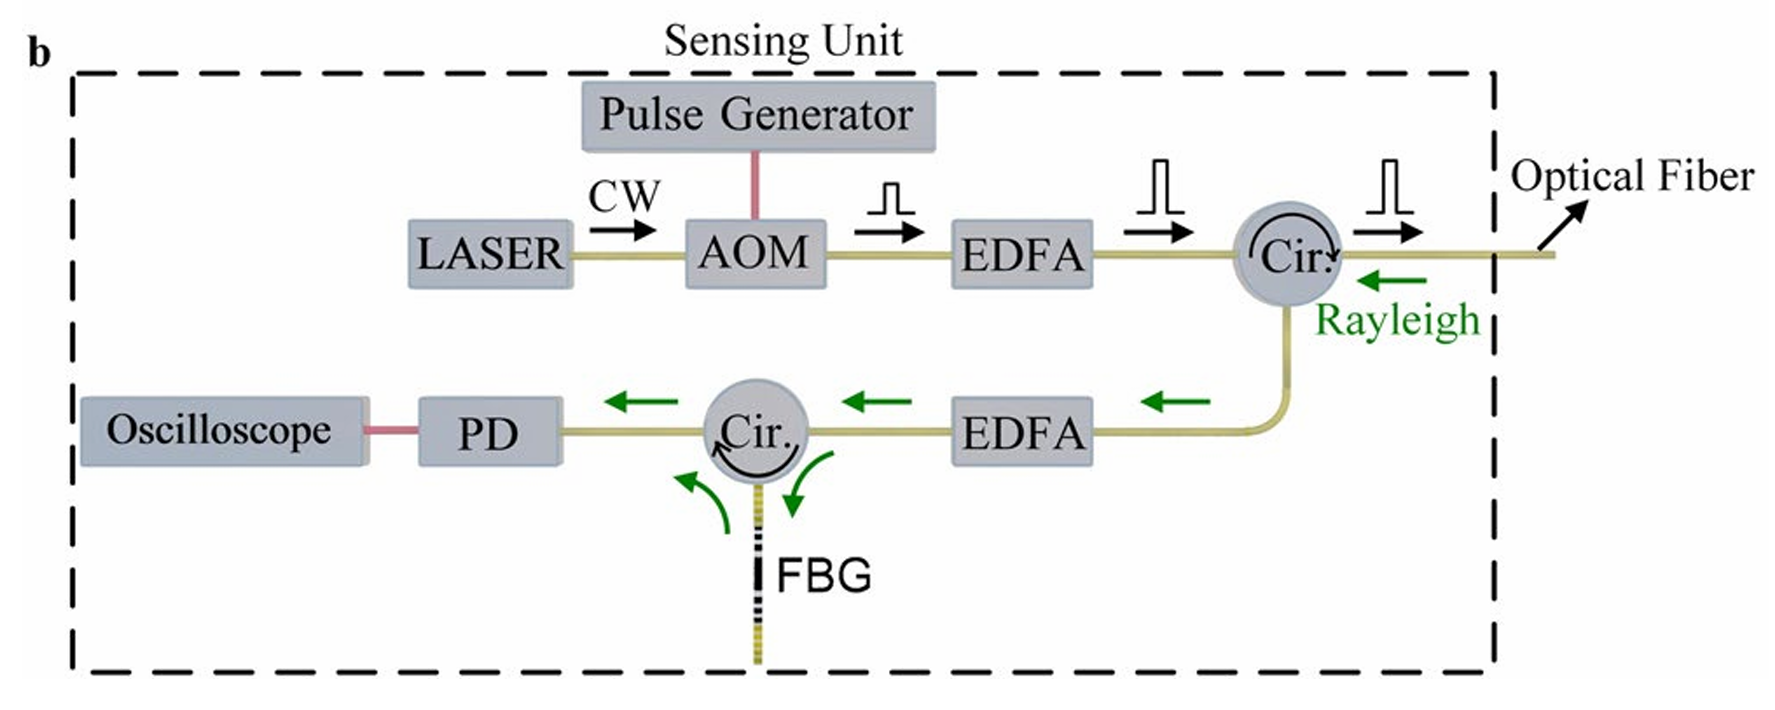
\includegraphics[width=0.75\textwidth]{figures/fig5_das_architecture.png}
\caption{DAS System Architecture \cite{wang2021}}
\label{fig:das_architecture}
\end{figure}

In phase-sensitive optical time-domain reflectometry ($\Phi$-OTDR), one continuous fiber is wrapped around the exterior of multiple trunks. A DAS interrogator measures changes in Rayleigh backscatter caused by local vibration and identifies the disturbance position along the fiber \cite{ashry2020,wang2021}. This provides distributed, non-invasive coverage without drilling each tree. Published work presents large-farm coverage as a design advantage, but the cited experiments do not demonstrate routine monitoring of 1,000 or more live trees; that scale should therefore be treated as projected capacity rather than validated deployment.

Signal processing in DAS-based systems follows a pipeline broadly analogous to that used in contact probe systems. Raw time-domain Rayleigh traces are differenced against a reference to extract acoustic perturbations, and a band-pass filter spanning 100 to 800 Hz is applied to suppress low-frequency environmental noise such as tree swinging caused by wind and high-frequency electronic noise from the sensing hardware, while preserving the dominant spectral content of larval feeding sounds \cite{ashry2022cnn,wang2021}. The filtered signals are then organized as two-dimensional matrices of spatial points versus temporal or spectral samples and passed to convolutional neural network (CNN) classifiers trained through supervised learning to distinguish infested from healthy tree signatures \cite{ashry2022cnn,wang2021,mao2021}.

Published DAS studies report strong signal-classification results within their experimental settings. Ashry et al. reported 97.0\% accuracy for temporal data and 97.1\% for spectral data using signals collected from controlled and outdoor-farm experiments \cite{ashry2022cnn}. Earlier laboratory work using simulated RPW sound also reported accuracies above 99\% \cite{wang2021}. Requiring temporal and spectral classifiers to agree reduced the reported false-alarm metric by about 20\% \cite{ashry2022cnn}. These metrics apply to the studied signals and conditions; they should not be interpreted as proven whole-farm detection accuracy.

A controlled indoor experiment detected larvae approximately 12 days old, and the later field study used larvae less than three weeks old \cite{ashry2020,ashry2022cnn}. DAS can be operated continuously, but outdoor performance remains sensitive to wind. The field study reported its best results below about 9 mph and substantially more false alarms at higher wind speeds \cite{ashry2022cnn}. Wider deployment therefore requires stronger field validation and improved handling of wind-induced vibration.

\section{Non-Acoustic Detection Methodologies}
\label{sec:GRP-III}

This section examines alternative sensing methodologies beyond acoustic detection. Prior studies have investigated a range of approaches, including chemical, molecular, and pheromone-based sensing techniques. Evaluating these alternatives was essential to ensure that the most appropriate sensing methodology was selected for the proposed system.

\subsection{Volatile Organic Compound (VOC) Biosensing}

Chemical detection strategies for \textit{Rhynchophorus ferrugineus} rely on the identification and sensing of volatile organic compounds and other biochemical signatures associated with larval feeding and metabolic activity within date palm tissues. These approaches exploit the fact that infestation induces measurable chemical changes in the host tree and that the insect itself emits characteristic volatile compounds during development.

A whole-cell bacterial biosensor was evaluated as a proof of concept for detecting volatile changes associated with RPW-infested material and date palms \cite{harpaz2022}. The genetically modified bacteria produced a bioluminescent stress response when exposed to air near tested samples. The study demonstrates that VOC-related biological responses can distinguish tested infested and uninfested samples, but it does not establish a field-ready sensor or identify a single infestation-specific compound. Commercial measurement equipment and controlled exposure were still required.

\begin{figure}[H]
\centering
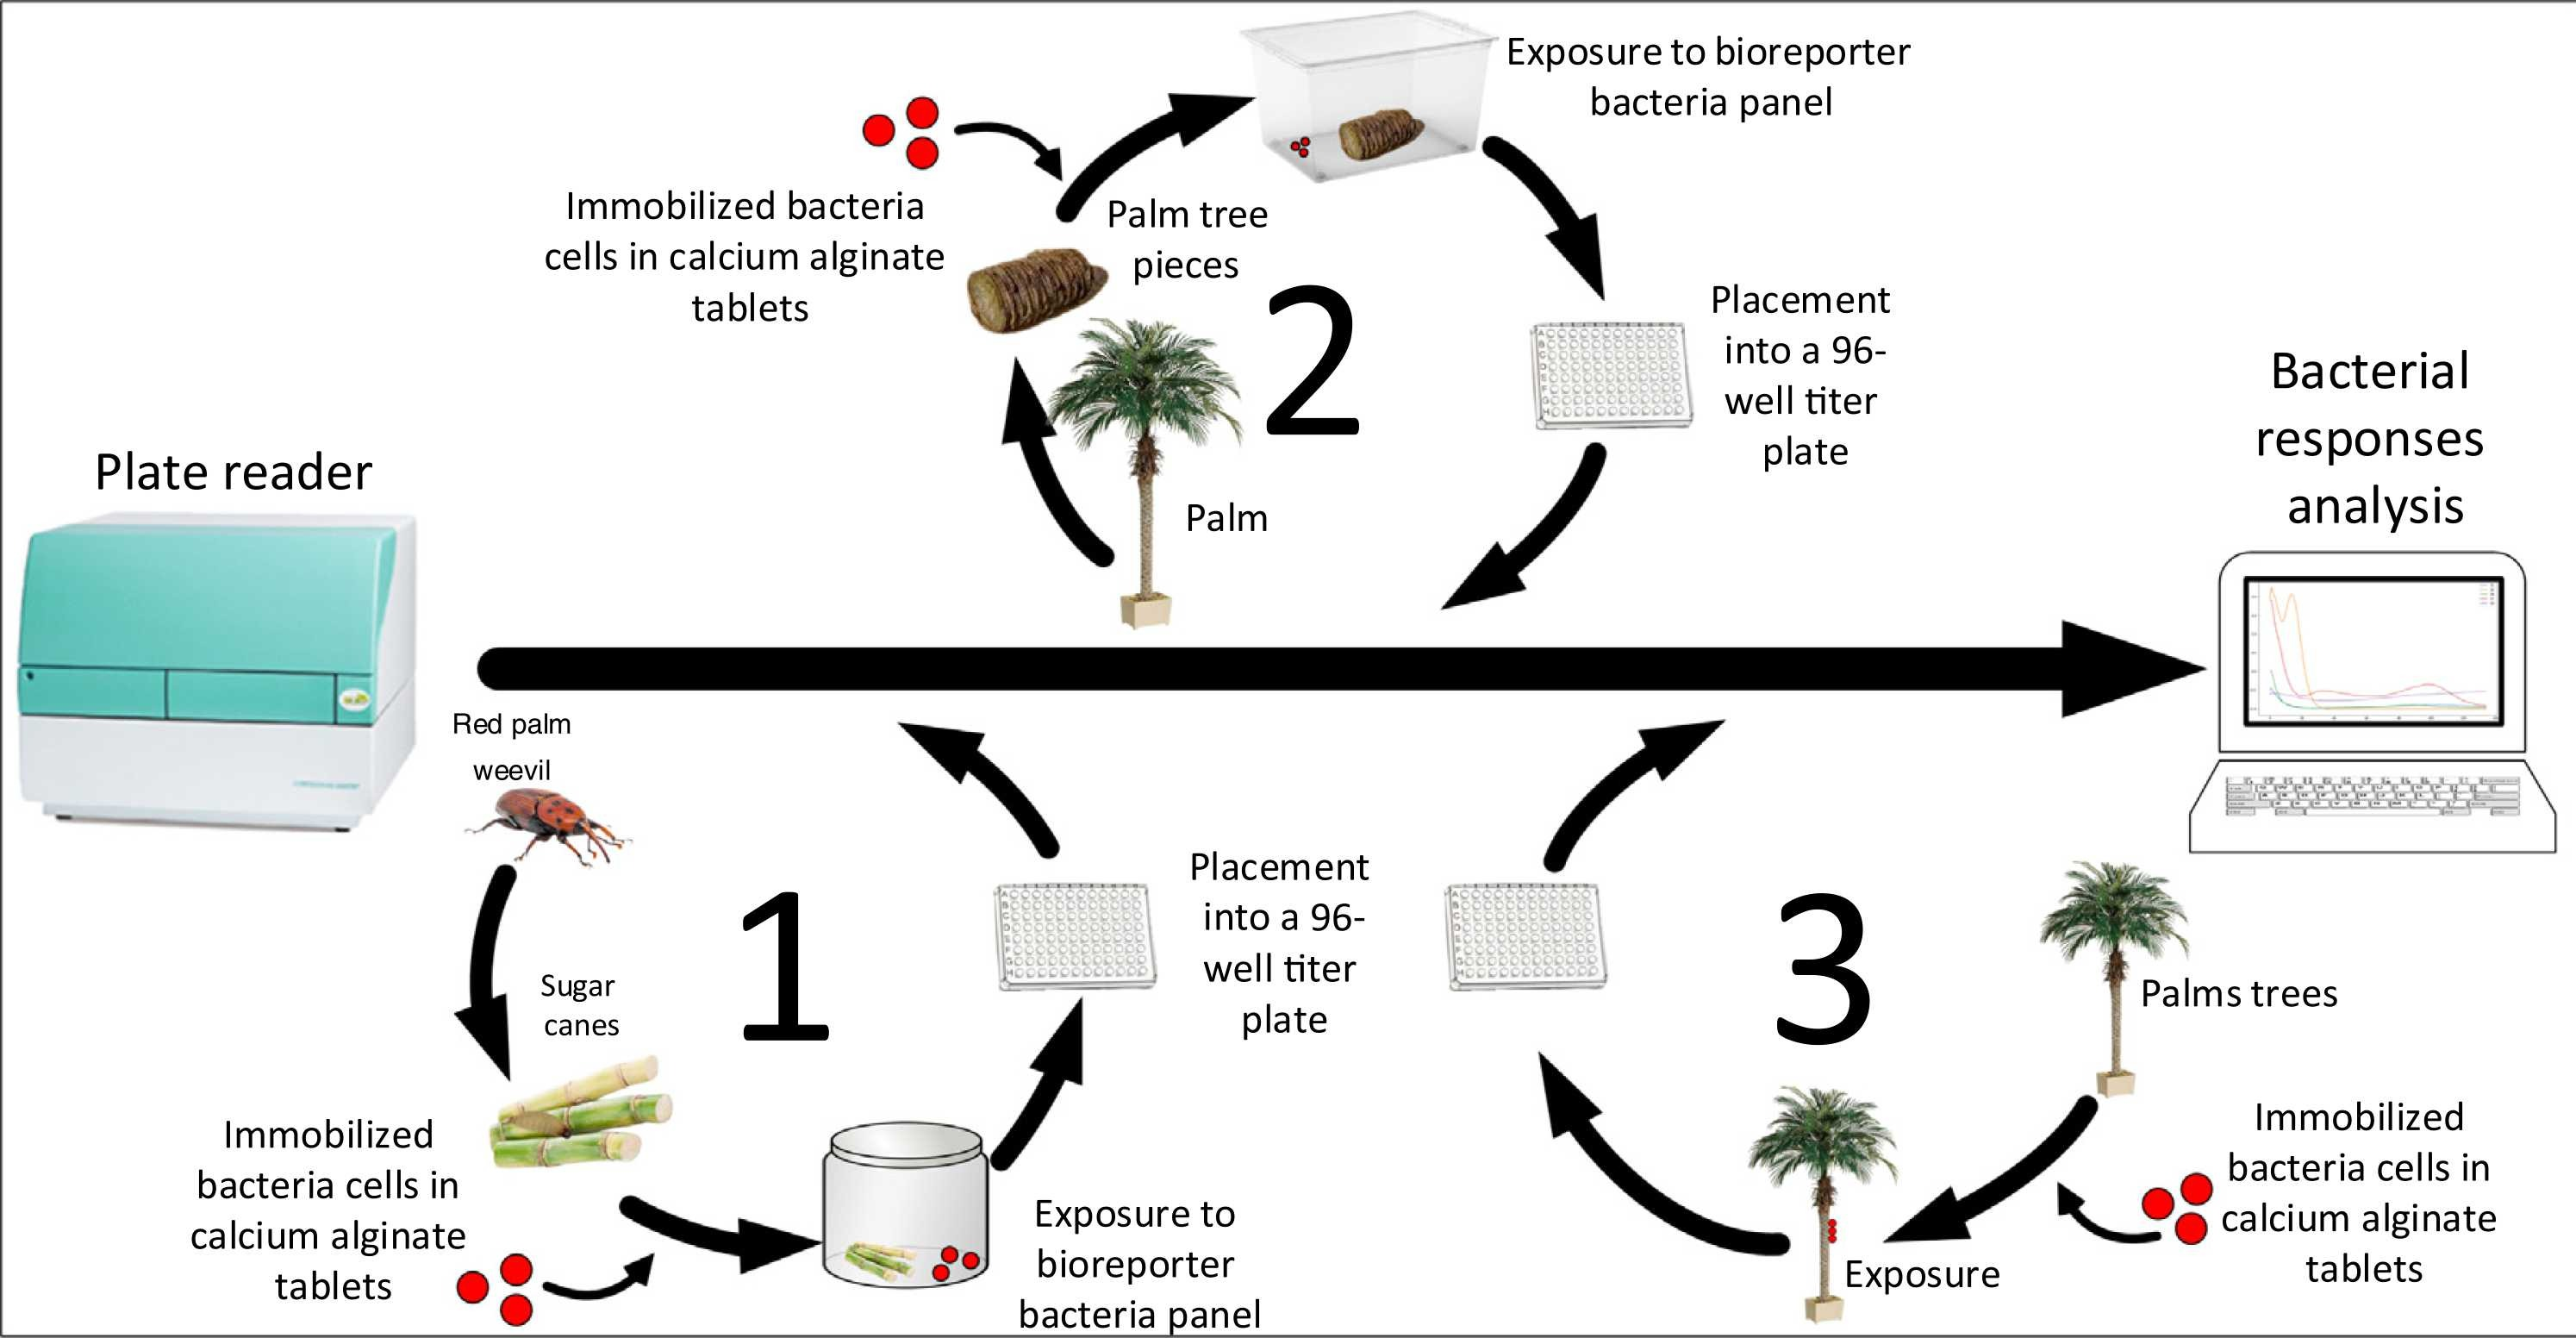
\includegraphics[width=0.99\textwidth]{figures/fig6_biosensor_schematic.png}
\caption{Schematic of The Experiment \cite{harpaz2022}}
\label{fig:biosensor_schematic}
\end{figure}

The chemical ecology of red palm weevil larvae further supports the feasibility of volatile-based detection. Detailed characterization of larval volatiles revealed stage-dependent emission profiles composed of specific chemical constituents that vary with developmental phase and pathogen stress \cite{ding2025}. The study identified distinct volatile organic compounds emitted by larvae and quantified their emission dynamics under varying biological conditions \cite{ding2025}. These findings indicate that larval metabolic processes generate a reproducible chemical fingerprint that can serve as a diagnostic indicator of infestation. Moreover, changes in volatile composition in response to physiological stress suggest that chemical emissions are sensitive to biological activity, potentially enabling differentiation between active and inactive infestations.

Together, volatile profiling and biosensing offer a possible route to non-destructive chemical screening \cite{harpaz2022,ding2025}. Their present maturity is limited: the cited work is proof-of-concept or laboratory research, and selectivity, sensor lifetime, calibration, field packaging, and false-positive control still require validation. The literature therefore supports VOC biosensing as a research alternative, not as an established continuous farm-monitoring method.

\subsection{Molecular Markers}

The cited molecular studies characterize RPW populations and support species identification; they do not directly detect hidden infestation inside a living palm. Molecular methods can confirm that a collected insect or biological sample belongs to \textit{Rhynchophorus ferrugineus}, but they first require representative material to be found and sampled.

Sabit et al. compared RPW samples from the Eastern Province of Saudi Arabia using RAPD and ISSR fingerprinting to study genetic relationships and possible population origins \cite{sabit2021}. The work is useful for population characterization and pest-management research, but it did not validate an assay for diagnosing infestation from palm tissue.

El-Zoghby et al. likewise examined genetic variability and ultrastructural traits in adult RPW collected from different locations in Egypt \cite{elzoghby2022}. Those results may inform later assay design, but the study addressed population differences and taxonomic characterization rather than early tree-level detection.

Molecular analysis may provide high-specificity confirmation when suitable biological material is available. However, the two cited studies do not support claims of low-level infestation detection, rapid screening of suspect trees, or portable on-site diagnosis. For this project, molecular methods are therefore considered a complementary confirmation approach rather than an alternative continuous-monitoring architecture.

\subsection{Pheromone Trap}

Pheromone-based detection exploits the aggregation behavior of \textit{Rhynchophorus ferrugineus}, which relies on chemical communication mediated by pheromones and synergistic attractants. By deploying optimized lure formulations and trap configurations, the presence of adult weevils in an area can be detected before widespread infestation occurs.

Optimization of pheromone trapping systems in Saudi Arabia demonstrated that trap performance is significantly influenced by lure composition, trap placement, and environmental factors \cite{shukla2018}. The study evaluated different trap contents and spatial arrangements, establishing conditions that maximize adult capture rates \cite{shukla2018}. Since adult weevils are responsible for dispersal and oviposition, their capture serves as an early indicator of infestation risk within a plantation. Effective trap optimization improves sensitivity, enabling detection of low-density populations.

Further assessment of attractant combinations in the United Arab Emirates examined the synergistic effects of pheromones with additional kairomonal components \cite{na2024}. The evaluation of different attractant mixtures demonstrated that specific combinations significantly enhance trap efficacy, increasing the probability of detecting active populations \cite{na2024}. Enhanced attractant formulations improve signal strength in surveillance programs by increasing adult aggregation around traps. This allows detection even when infestation levels are initially low.

\begin{figure}[H]
\centering
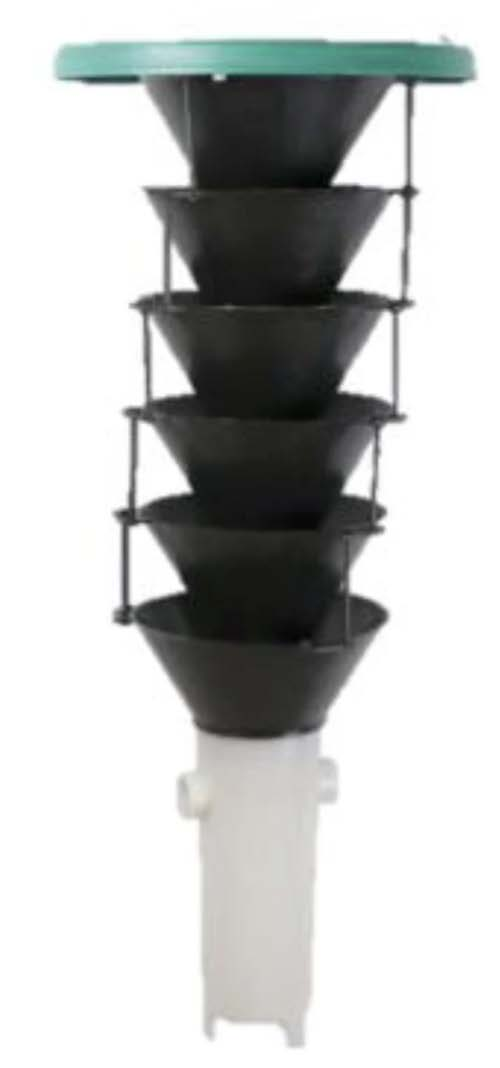
\includegraphics[width=0.2\textwidth]{figures/fig7_pheromone_traps.jpeg}
\caption{The Traps used in the Experiments \cite{na2024}}
\label{fig:pheromone_traps}
\end{figure}

Pheromone trap systems function as indirect detection mechanisms by capturing dispersing adults, thereby providing spatial information about infestation hotspots. Data collected from optimized traps can be used to map population distribution and monitor seasonal dynamics. The combined findings from trap optimization studies and attractant assessment experiments demonstrate that chemical communication pathways can be systematically leveraged for surveillance \cite{shukla2018,na2024}. Properly calibrated pheromone trapping networks enable early identification of infestation zones, facilitate targeted intervention, and support continuous monitoring of red palm weevil activity.

\section{Signal Processing Algorithms for Acoustic Data Processing of RPW}

The reliable detection of Red Palm Weevil (RPW) larvae through acoustic sensing depends not only on the quality of the hardware used to capture vibrational signals, but critically on the signal processing pipeline applied to raw acoustic data. Because larval feeding sounds are low-amplitude, intermittent, and embedded within a background of environmental noise, a sequence of carefully designed processing stages is required to extract meaningful features from the raw signals. The literature identifies a consistent pipeline consisting of preprocessing and filtering, followed by time-frequency feature extraction.

\subsection{Preprocessing and Bandpass Filtering}

Raw acoustic signals captured by piezoelectric contact microphones or similar transducers are typically sampled at rates ranging from 8 kHz to 44 kHz. Prior to any feature extraction, the signals undergo digital bandpass filtering to isolate the frequency of band of interest and suppress noise sources that fall outside the larval acoustic signature. The commonly applied bandpass range spans 100 to 2500 Hz, which encompasses the dominant chewing and movement sounds produced by RPW larvae while rejecting low-frequency interference such as wind-induced vibrations, ground tremors, and machinery noise below 100 Hz, as well as high-frequency electronic noise above the band of interest \cite{pinhas2008,rach2013}. This filtering stage is foundational to all subsequent processing steps, as it directly determines the signal-to-noise ratio of the features passed to any downstream analysis.

\subsection{Signal Squaring and Moving Average}

Following bandpass filtering, a common energy-based processing step involves squaring the time-domain signal to convert it into a strictly positive power envelope, which accentuates the amplitude differences between larval activity bursts and background noise. A moving average is then applied to the squared signal over a sliding time window typically 100 ms to smooth instantaneous noise spikes and reveal the underlying temporal pattern of larval feeding activity. This approach exploits the on/off feeding behavior of RPW larvae, which produces characteristic ups and downs in the moving average output when larvae are active, in contrast to the relatively flat and constant moving average observed from healthy trees. The complete signal processing pipeline, from raw signal acquisition through to the final infestation decision, is illustrated in Figure~\ref{fig:signal_pipeline} \cite{wang2021}.

\begin{figure}[H]
\centering
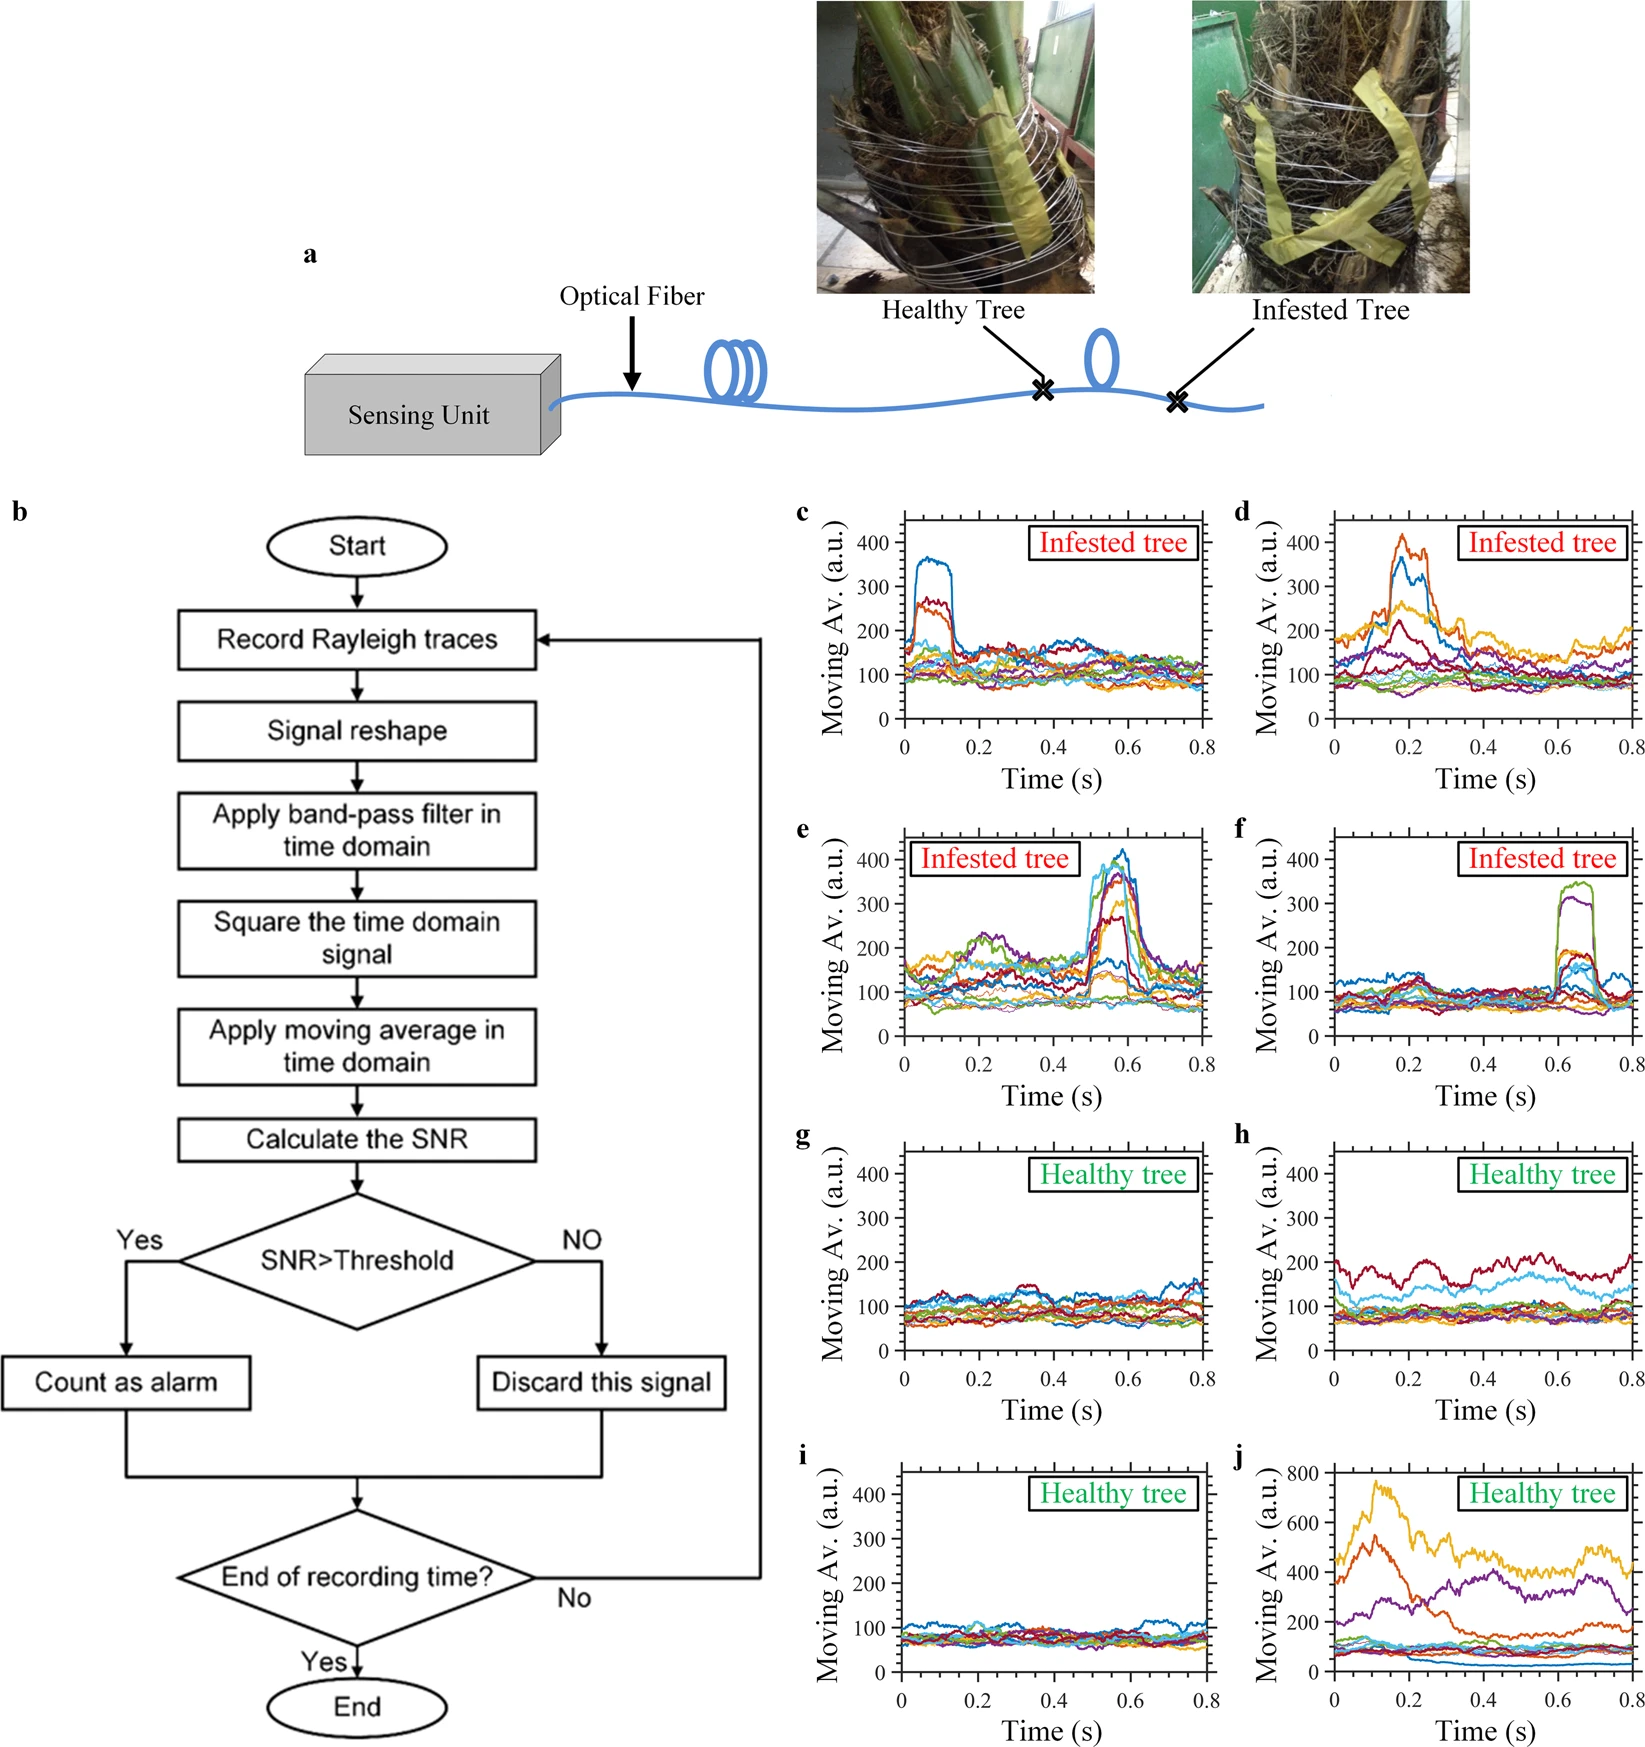
\includegraphics[width=0.99\textwidth]{figures/41598_2020_60171_Fig4_HTML.png}
\caption{Flowchart of the signal processing and detection algorithm \cite{ashry2020}}
\label{fig:signal_pipeline}
\end{figure}

\subsection{Signal-to-Noise Ratio Thresholding}

After the moving average is computed, an SNR-like measure compares its high and low levels within each window. A window above the selected threshold is counted as an infestation alarm. The threshold must be calibrated for the sensor and environment rather than treated as universal. In one controlled DAS experiment, a 4 dB threshold produced 97 alarm counts for an infested tree and 9 for a healthy tree during a two-hour recording \cite{ashry2020}.

\subsection{Short-Time Fourier Transform and Spectrogram Representation}

A widely adopted alternative approach for converting time-domain acoustic signals into a form suitable for further analysis is the Short-Time Fourier Transform (STFT). The STFT divides the filtered signal into short, overlapping temporal windows and computes the Fourier transform of each window, yielding a two-dimensional time-frequency representation known as a spectrogram. The spectrogram encodes how the energy distribution across frequencies evolves over time, revealing the characteristic intermittent burst patterns associated with larval feeding \cite{pinhas2008,rach2013}. This representation is particularly valuable because it preserves both the spectral content and the temporal structure of the acoustic signal simultaneously, making the distinct impulsive nature of larval chewing sounds visually and mathematically distinguishable from more continuous environmental noise sources. Deep learning models applied to spectrogram inputs have demonstrated strong classification performance for RPW detection, with studies reporting accuracies exceeding 97\% under controlled conditions \cite{boulila2023}.

\subsection{Cepstral Feature Extraction}

An alternative and complementary approach to spectrogram-based representation is cepstral feature extraction. Mel-Frequency Cepstral Coefficients (MFCCs) compress the spectral content of an acoustic signal into a compact vector representation by mapping the power spectrum onto the mel frequency scale a perceptual scale that approximates the non-linear frequency response of the human auditory system and then applying a discrete cosine transform. Similarly, Bark Frequency Cepstral Coefficients (BFCCs) apply the same principle using the Bark psychoacoustic scale, and Constant Q Cepstral Coefficients (CQCCs) use a constant-Q frequency resolution that provides higher frequency resolution at lower frequencies. All three representations produce compact, noise-robust spectral descriptors that suppress redundant fine spectral detail while retaining the envelope shape most characteristic of the acoustic source \cite{pinhas2008,rach2013,boulila2023}. Studies have shown that concatenating MFCC, BFCC, and CQCC features before classification outperforms using any single feature extraction technique in isolation, yielding superior results across multiple acoustic datasets \cite{boulila2023}. Linear Predictive Coding (LPC) offers a further alternative, modeling the acoustic propagation channel through the wood structure as an autoregressive filter whose coefficients summarize the spectral envelope of the signal in a small set of parameters. LPC is computationally efficient and has been shown to effectively capture the resonance characteristics of larval feeding sounds as they propagate through palm trunk tissue \cite{saranya2025}.

\subsection{Comparative Assessment}

Each feature extraction approach involves trade-offs between computational complexity, compactness, and robustness to environmental noise. The SNR-based moving average approach is computationally lightweight and well-suited to real-time embedded deployment but is most effective when larval feeding produces clearly intermittent amplitude patterns and may be susceptible to false alarms under highly variable noise conditions \cite{wang2021}. STFT spectrograms preserve the most complete time-frequency information but produce large two-dimensional representations that carry higher computational cost in downstream processing \cite{boulila2023}. Cepstral features such as MFCCs, BFCCs, and CQCCs are significantly more compact and computationally lighter, and their combination has demonstrated particularly strong generalization across different acoustic environments \cite{boulila2023}. LPC coefficients are the most compact representation and least computationally demanding, making them attractive for embedded or IoT-constrained deployment scenarios \cite{saranya2025}. For real-world farm deployment, where wind, rain, bird activity, and mechanical noise are unavoidable, selecting the appropriate feature representation for the prevailing noise environment is a critical design decision that directly affects detection reliability \cite{pinhas2008,rach2013,saranya2025}.

\section{Deep Learning for Acoustic Data Classification of RPW Infestation}

\subsection{CNN Transfer Learning for Acoustic Signal Classification}

Transfer learning allows a CNN pre-trained on a large image dataset to classify image-like acoustic representations with less task-specific data. Karar et al. applied InceptionResNet-V2 to TreeVibes and reported 97.18\% accuracy on their train/test split and $94.53\% \pm 1.69\%$ under 10-fold cross-validation \cite{karar2021}. TreeVibes contains short recordings of several wood-boring insects, not exclusively RPW, and the study assumed that infested date-palm recordings represented RPW activity \cite{rigakis2021,karar2021}. This label limitation must be considered when interpreting the results.

In another study, the authors improved this approach by applying audio feature extractors to the raw audio signal before feeding the extracted features into transfer learning CNN models \cite{boulila2023}. The selected audio features were Mel-frequency cepstral coefficients (MFCC), Constant Q cepstral coefficients (CQCC), and Bark frequency cepstral coefficients (BFCC). Each of these feature extraction techniques generates a two-dimensional image representing the extracted features. These three feature images are concatenated and fed into one of the following transfer learning (TL) models: MobileNetV2, ResNet50V2, ResNet152V2, VGG16, VGG19, DenseNet121, DenseNet201, Xception, and InceptionV3.

The final feature vector output by a TL model is then fed into a classifier to determine whether the palm tree is infested. A research paper provided the following diagram to illustrate the full pipeline, from the audio signal to classification \cite{boulila2023}.

\begin{figure}[H]
\centering
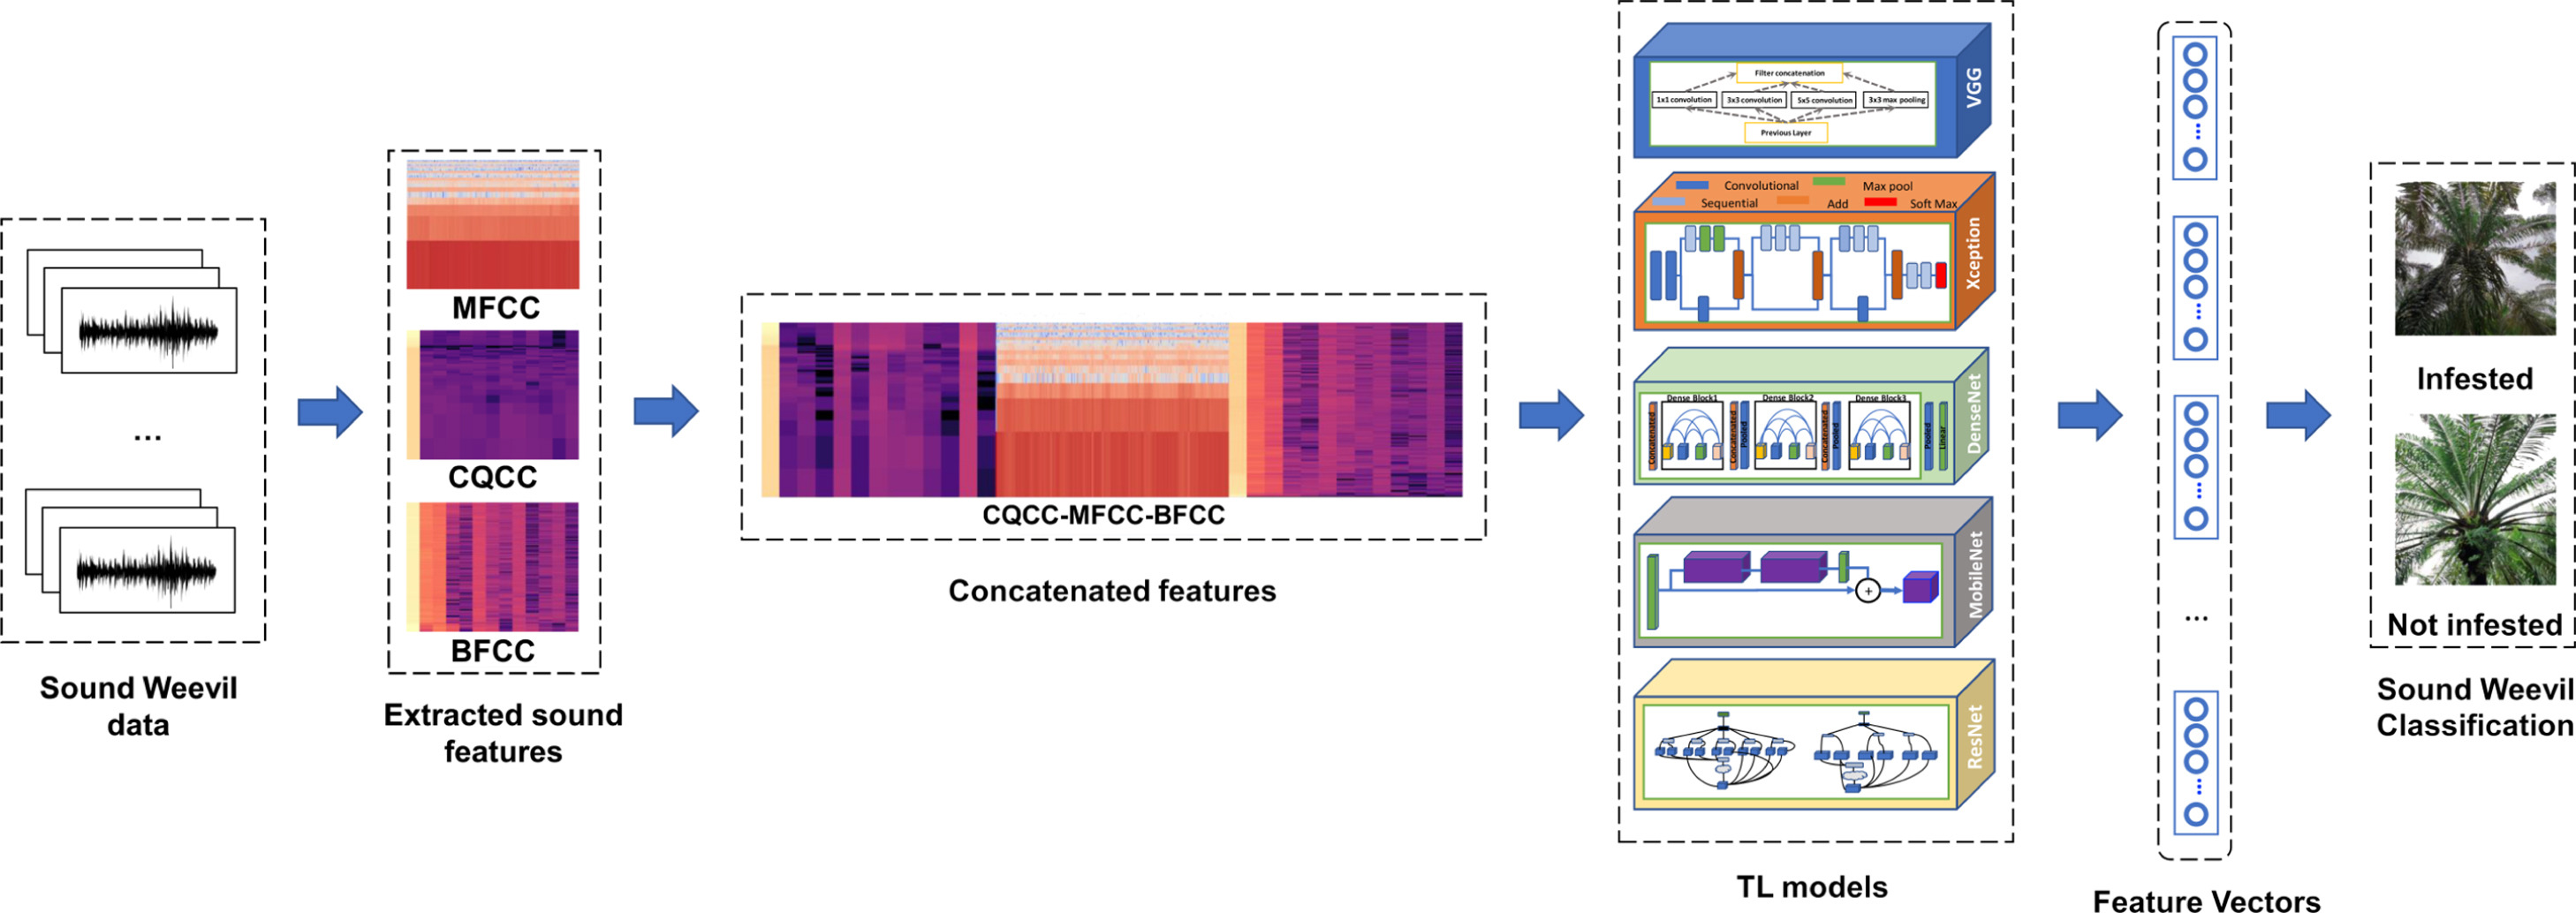
\includegraphics[width=0.99\textwidth]{figures/fig9_cnn_pipeline.jpg}
\caption{Full Model Pipeline \cite{boulila2023}}
\label{fig:cnn_pipeline}
\end{figure}

On the RPW dataset used by Boulila et al., combined CQCC, MFCC, and BFCC images generally outperformed single-feature inputs across the evaluated CNNs \cite{boulila2023}. The same feature combination achieved 0.95 accuracy, 0.947 precision, 1.0 recall, and a 0.973 F1 score on ESC-10 \cite{boulila2023}. Results on general environmental-sound datasets support the feature-fusion method, but they are not direct evidence of RPW field performance.

These results make cepstral feature fusion with transfer-learning CNNs a reasonable candidate for comparison in this project. Its value must still be tested on representative RPW field recordings with tree-level data separation.

\subsection{Bidirectional Long Short Term Memory Models for RPW Detection Through Acoustic Detection}

Another paper proposed a Bidirectional Long Short-Term Memory (BiLSTM) architecture for detecting RPW infestation from acoustic signals \cite{saranya2025}. The study introduced a complex, multistage data preprocessing pipeline, beginning with initial noise suppression to remove environmental noise such as wind. This is followed by Linear Predictive Coding (LPC), which extracts ``compact and discriminative'' spectral features from the audio signals that are specific to RPW activity.

Next, cosine similarity is computed between the extracted features and reference RPW and non-RPW vectors. The resulting cosine similarity coefficients are stored in a matrix, where each row corresponds to an audio file and each column contains similarity values. This matrix is then fed into a Bidirectional LSTM architecture, meaning that the temporal signal is processed by both a conventional forward LSTM and a backward (end-to-start) LSTM. The outputs of the forward and backward LSTMs are concatenated and passed to a dense layer for classification.

The researchers reported a classification accuracy of 98.02\%. They attributed the success of this approach in noisy environments to the ``combination of LPC feature extraction, cosine similarity-based feature matching, and a Bi-LSTM architecture.''

\subsection{Comparing RNNs and CNNs}

The researchers compared the use of CNNs and LSTM-based RNNs for environmental audio classification using the FSDKaggle2018 and ESC-50 datasets \cite{rezaul2024,fonseca2018}. Mel Frequency Cepstral Coefficients (MFCC) were used as a feature extractor, and the resulting feature vectors were fed into either a CNN or an LSTM model.

The ESC-50 CNN architecture used consisted of 10 layers, including convolutional layers with varying numbers of filters (ranging from 16 to 128), a filter size of 3, and ReLU activation, along with max-pooling, dropout, and dense layers for classification \cite{rezaul2024}. The LSTM architecture for ESC-50 consisted of 13 layers, including ``LSTM units, Batch Normalization, and Dropout layers.'' Time-distributed dense layers were also used, followed by a dense multi-class classifier layer.

The researchers reported that CNNs performed better than LSTMs on the smaller FSDKaggle2018 dataset, achieving 96.52\% and 87.88\% test accuracy, respectively \cite{rezaul2024,fonseca2018}. However, LSTMs performed better on the ESC-50 dataset, achieving 92.89\% accuracy compared to 88.47\% for CNNs \cite{rezaul2024}.

\subsection{CNN-LSTM Hybrid Architecture}

Another study proposed a hybrid CNN-LSTM model for environmental audio classification. This architecture uses 1D CNNs as feature extractors and feeds the extracted features into an LSTM block to capture time-based sequential relationships. A fully connected layer is then used for classification. Dropout layers are applied before the LSTM layer and before the fully connected layer. Max-pooling and ReLU activation are used after each convolutional layer. Figure~\ref{fig:cnn_lstm} illustrates the hybrid CNN-LSTM architecture presented in \cite{akter2025}.

\begin{figure}[H]
\centering
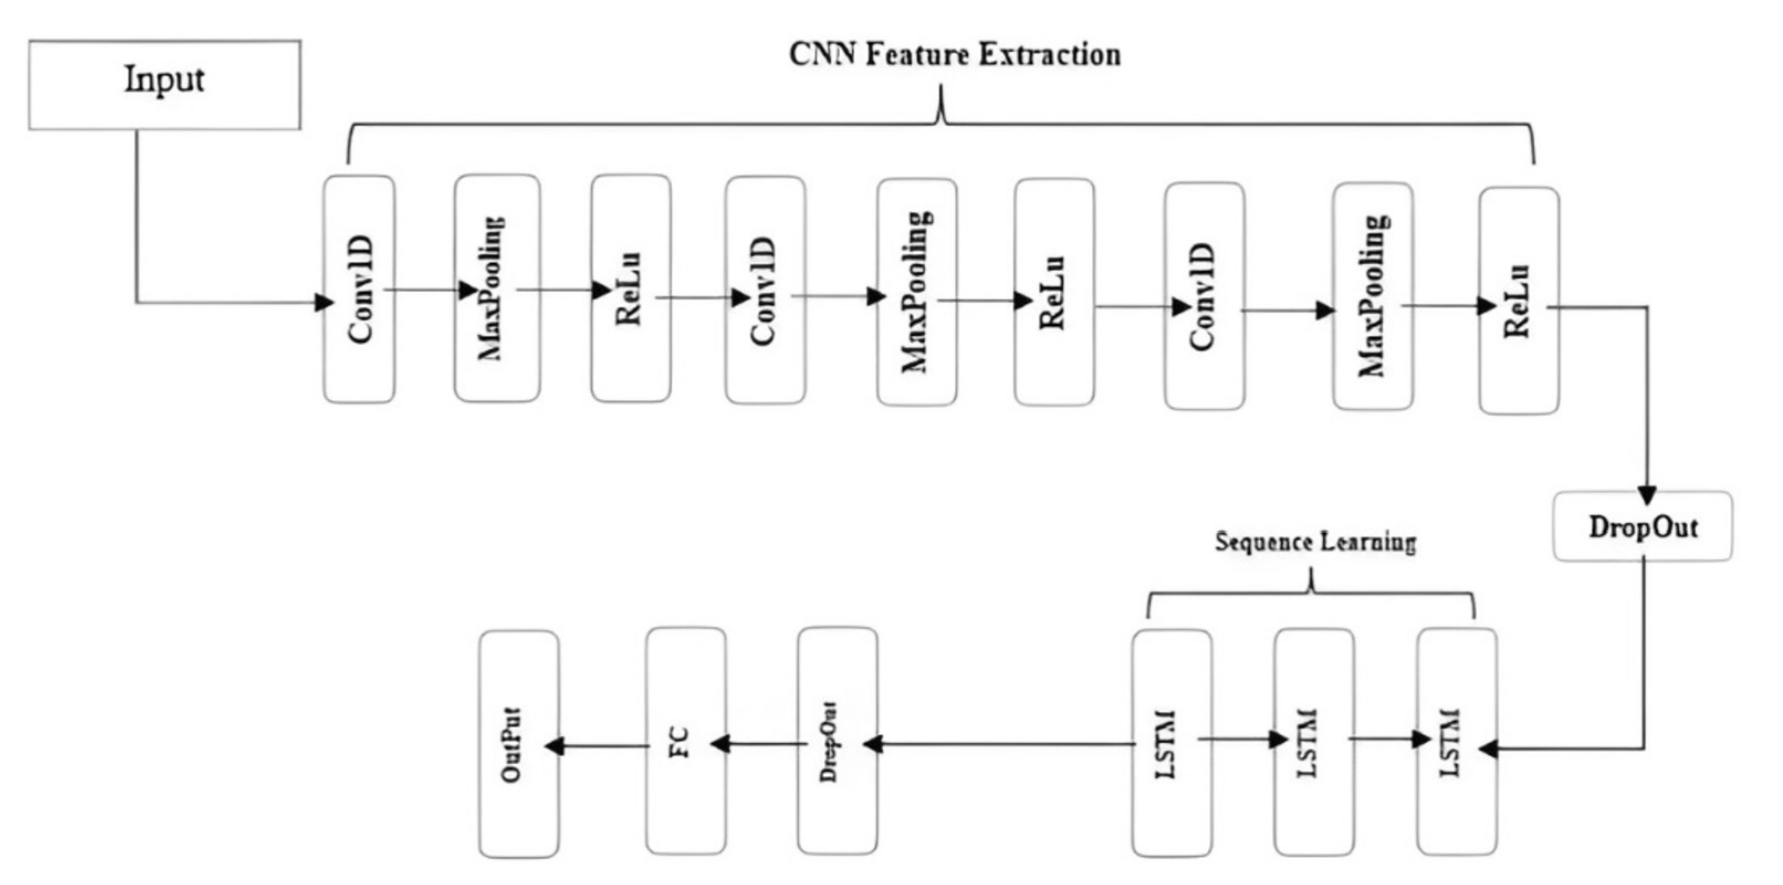
\includegraphics[width=0.85\textwidth]{figures/fig2_6_replacement.png}
\caption{CNN-LSTM Hybrid Model Architecture \cite{akter2025}}
\label{fig:cnn_lstm}
\end{figure}

The model reported 99.33\% accuracy on ESC-50 and 98.38\% on UrbanSound8K \cite{akter2025}. These are environmental-sound results, not RPW results. They justify evaluating a CNN-LSTM baseline, but they do not show that the same accuracy will transfer to trunk vibrations. Combining that architecture with the MFCC, BFCC, and CQCC features studied by Boulila et al. is a testable project hypothesis rather than an established improvement \cite{boulila2023}.

\renewcommand{\arraystretch}{1.1}
\begin{landscape}
\scriptsize
\renewcommand{\arraystretch}{1.3}
\setlength{\tabcolsep}{6pt}

% Center the longtable on the page
\setlength\LTleft{\fill}
\setlength\LTright{\fill}

\begin{longtable}{@{}
    >{\raggedright\arraybackslash}p{2.8cm}
    >{\centering\arraybackslash}p{1.0cm}
    >{\raggedright\arraybackslash}p{1.8cm}
    >{\raggedright\arraybackslash}p{2.5cm}
    >{\raggedright\arraybackslash}p{9.5cm}
    >{\raggedright\arraybackslash}p{1.6cm}
    >{\raggedright\arraybackslash}p{2.0cm}@{}}
\caption{Summary of RPW Audio Classification Techniques adapted from the comparative review in \cite{boulila2023}}\label{tab:rpw_summary}\\
\toprule
\textbf{Ref.} & \textbf{Year} & \textbf{Algorithm} & \textbf{Data Type} & \textbf{Steps} & \textbf{Dataset} & \textbf{Accuracy} \\
\midrule
\endfirsthead
\caption[]{Summary of RPW Audio Classification Techniques (continued)}\\
\toprule
\textbf{Ref.} & \textbf{Year} & \textbf{Algorithm} & \textbf{Data Type} & \textbf{Steps} & \textbf{Dataset} & \textbf{Accuracy} \\
\midrule
\endhead
\bottomrule
\endfoot
\bottomrule
\endlastfoot

Pinhas et al. (2008) & 2008 & GMM, VQ & Spectral &
\textbullet\ Record the RPW using off-the-shelf devices \newline
\textbullet\ Manually label the data \newline
\textbullet\ Calculate the noise threshold \newline
\textbullet\ Count mismatched labels
& -- & 98.8\%, 98.9\% \\
\addlinespace

Parvathy et al. (2021) & 2021 & CAE & Mel Spectrograms &
\textbullet\ Capture audio signals \newline
\textbullet\ Extract features using the Mel spectrogram algorithm \newline
\textbullet\ Convert the features to images \newline
\textbullet\ Train the CAE on the images
& -- & 95.8\% \\
\addlinespace

Mohamed et al. (2021) & 2021 & AlexNet & MFCC &
\textbullet\ Extract features using the MFCC algorithm \newline
\textbullet\ Convert the features to images \newline
\textbullet\ Train AlexNet on the images
& -- & 99.2\% \\
\addlinespace

Wang et al. (2021) & 2021 & ANN, CNN & Temporal, Spectral &
\textbullet\ Install a fiber-optic DAS system on palm trees \newline
\textbullet\ Capture audio signals \newline
\textbullet\ Train ANN and CNN models with the DAS data \newline
\textbullet\ Evaluate laboratory data with simulated RPW sound
& -- & 99.9\%, 99.7\% \\
\addlinespace

Ashry et al. (2022) & 2022 & CNN & Temporal, Spectral &
\textbullet\ Record RPW sounds using DAS \newline
\textbullet\ Transform them into temporal and spectral data \newline
\textbullet\ Train CNN models on the data separately \newline
\textbullet\ Merge the CNN models
& -- & 97.0\%, 97.1\% \\
\addlinespace

Esmail Karar et al. (2022) & 2022 & CNN & Spectral &
\textbullet\ Extract spectral features \newline
\textbullet\ Convert the features to images \newline
\textbullet\ Train MixConvNet on the images \newline
\textbullet\ Compare performance with other models
& TreeVibes & 97.3\% \\

\end{longtable}
\end{landscape}

\section{Conclusions from Literature Survey}
\label{sec:Survey-Conclusion}

\earlierrevision{The literature supports acoustic, optical, chemical, molecular, and pheromone-based approaches to RPW monitoring, but it does not identify one method that is simultaneously inexpensive, non-invasive, field-proven, and scalable.}

\earlierrevision{Probe-based acoustic systems use relatively simple hardware and can detect larval vibration, but many designs require a drilled waveguide, sense only a limited area, and remain sensitive to field noise. Reported machine-learning accuracies are encouraging, yet they come from different datasets and experimental protocols and cannot be compared as if they measured the same task.}

\earlierrevision{DAS provides non-invasive distributed coverage and has detected young larvae in controlled and outdoor experiments. Its main barriers are the interrogator, fiber installation, and wind-induced false alarms. VOC biosensing remains at proof-of-concept maturity. The cited molecular studies support species and population characterization, not direct diagnosis of hidden infestation in a live tree. Pheromone traps are useful for monitoring adult populations but do not confirm larval activity in a particular trunk.}

\earlierrevision{These findings support the project's central choice: evaluate a lower-cost, minimally invasive piezoelectric node with local feature extraction, LoRa communication, and cloud classification. The design does not assume that laboratory accuracy will transfer directly to farms. Its contribution is to test whether a modular prototype can achieve useful field performance at a lower infrastructure cost, while reporting noise sensitivity, installation effort, coverage, false negatives, and total deployment cost as explicit limitations.}

\chapter{System Specifications}
\label{ch:Specifications}
 
% ===============================
% CHAPTER 3: SYSTEM SPECIFICATION
% ===============================
 
\section{Functional Requirements}
\label{sec:FR}
 
\earlierrevision{FR1: The sensing node shall capture trunk vibrations with a piezoelectric sensor and digitize the conditioned signal with the ESP32.}

\earlierrevision{FR2: The sensing node shall apply signal conditioning, bandpass filtering, SNR gating, and MFCC feature extraction to each scheduled measurement.}

\earlierrevision{FR3: When the configured SNR threshold is exceeded, the sensing node shall transmit a LoRa packet containing the node ID, timestamp, acoustic features, and SNR value to the cluster head.}

\earlierrevision{FR4: The cluster head shall receive and locally log LoRa packets, then forward them to the cloud backend through MQTT over Wi-Fi or cellular connectivity.}

\earlierrevision{FR5: The cloud backend shall validate incoming features and use the selected trained model to classify each event as likely infested or healthy.}

\earlierrevision{FR6: The backend shall store acoustic features, classifications, alerts, and node and cluster-head health records in the time-series database.}

\earlierrevision{FR7: When the configured detection threshold is exceeded, the backend shall create an alert, record it, and send an email notification to authorized users.}

\earlierrevision{FR8: The dashboard shall display node and cluster-head status, locations, detection events, alerts, and historical trends.}

\earlierrevision{FR9: The dashboard and API shall require authenticated access to real-time and historical system data.}

\newrevision{FR10: The sensing node shall support a versioned compact binary packet and log the payload size and airtime for every transmission experiment.}

\newrevision{FR11: The project shall compare a baseline feature packet with at least one compacted MFCC packet and record payload bytes, airtime, packet loss, energy, and classification change.}

\newrevision{FR12: The bench apparatus shall follow the chain recording $\rightarrow$ amplifier $\rightarrow$ mechanically attached vibration exciter $\rightarrow$ wood/palm material $\rightarrow$ piezo sensor $\rightarrow$ MCP6002 $\rightarrow$ ESP32 $\rightarrow$ filtering/MFCC/classifier. A second reference piezoelectric sensor shall be mounted near the exciter to record the injected vibration.}

\newrevision{FR13: Controlled bench tests shall vary source-to-sensor distance, playback amplitude, and background vibration/noise or SNR. Each run shall retain its condition settings and measured results.}

\newrevision{FR14: The project shall compare the compact-feature baseline with one candidate split-learning point only when the ESP32 memory and runtime are feasible and the measured uplink cost is acceptable.}

\newrevision{FR15: Results from wood-plank or other emulation tests shall be labeled as bench validation. A live-RPW detection claim requires separately documented testing on naturally infested palms.}

\section{Non-Functional Requirements}
\label{sec:NFR}
 
\earlierrevision{NFR1: The acquisition and preprocessing pipeline shall preserve signals in the specified 100--2500 Hz band and shall be verified with known test signals.}

\earlierrevision{NFR2: Sensing nodes shall transmit extracted features rather than continuous raw audio during normal operation to reduce bandwidth and energy use.}

\earlierrevision{NFR3: The network shall support the number of prototype nodes defined in the validation plan. Capacity beyond the tested scale shall be reported as an estimate, not as demonstrated performance.}

\earlierrevision{NFR4: Communication reliability, packet loss, and end-to-end alert latency shall be measured under normal and interrupted-connectivity tests and reported against the validation criteria.}

\earlierrevision{NFR5: Cloud communication shall use encrypted transport, and dashboard and API access shall require authenticated, role-appropriate authorization.}

\earlierrevision{NFR6: The database shall return recent node status, classifications, and alert history within the response-time criteria defined in the validation plan.}

\earlierrevision{NFR7: The dashboard shall remain usable on current desktop and tablet browsers and shall clearly distinguish node health, detections, and acknowledged alerts.}

\earlierrevision{NFR8: The prototype enclosure and electronics shall be tested under the temperature, humidity, and dust conditions available in the project validation environment. Conditions not tested shall be stated as limitations.}

\newrevision{NFR9: The packet format shall include a version field so that compact-packet and split-learning experiments can be decoded and compared without ambiguity.}

\newrevision{NFR10: The reference and measurement sensors shall be calibrated or checked against the same injected signal before each controlled test series; the check method and any failed coupling condition shall be recorded.}
 
\section{External Interfaces and Database Requirements}
 
\subsection*{External Interfaces}
 
The RPW acoustic detection system interacts with external components spanning three distinct layers: the sensing layer, the cluster aggregation layer, and the cloud backend.
 
\subsubsection*{Sensor-to-Microcontroller Interface}
 
At each sensing node, the primary hardware interface is between the 27mm piezoelectric disc sensor and the ESP32 microcontroller. The piezoelectric element is in physical contact with the surface of the palm trunk and generates a low-amplitude analog voltage signal (mV range) that varies as a function of internal vibrations generated by larval feeding activity. The output signal is then fed into an MCP6002 op-amp amplification circuit, which brings the output value to a level suitable for ESP32's analog to digital converter (ADC) input range. The conditioned signal is then digitized by an ADC at a rate sufficient to capture the full RPW larval frequency band, known to range from 100 Hz to 2500 Hz \cite{pinhas2008,rach2013}, with a desired sampling rate of at least 8 kHz (i.e., well above the Nyquist limit).
 
\subsubsection*{Sensing Node-to-Cluster Head Interface}
 
\earlierrevision{Communication between sensing nodes and the cluster head uses HopeRF RFM95W LoRa modules. The current design assumes SF7, 900 ms TDMA slots, hourly nighttime wake-ups from 10 PM to 6 AM, and four-hour daytime wake-ups from 6 AM to 10 PM. During normal operation, raw audio remains on the node. The initial 4 dB SNR gate is drawn from a controlled DAS experiment and shall be recalibrated for the piezoelectric prototype rather than treated as a universal threshold \cite{ashry2020}. Airtime, payload limits, collisions, packet loss, regional radio settings, and duty-cycle constraints shall be measured before a supported node count is stated. The earlier estimate of 8,000 nodes per cluster head is therefore a planning calculation, not a validated requirement.}

\newrevision{The initial packet-format candidate contains a version, node identifier, timestamp, SNR value, and compact acoustic representation. Its final byte length, data rate, and airtime are experimental measurements, not fixed assumptions.}
 
\subsubsection*{Cluster Head-to-Cloud Interface}
 
Each cluster head uses a Raspberry Pi 4 and an RFM95W LoRa module. It remains on mains power, logs received feature packets locally, and forwards them to the cloud through MQTT over Wi-Fi or an available cellular backhaul. Each JSON message contains the node ID, UTC timestamp, SNR value, and MFCC vector. Classification remains in the cloud. Additional cluster heads can divide a plantation into zones, but capacity and radio range will depend on terrain, vegetation, antenna placement, interference, payload airtime, and permitted radio settings. The prototype shall report measured range and node capacity; it shall not claim a fixed 8,000-node block or 1 km field range without test evidence.
 
\subsubsection*{Cloud-to-Dashboard Interface}
 
The Cloud-to-Dashboard Interface is a web-based monitoring dashboard, and the cloud backend exposes a RESTful HTTP API to serve this data. Plantation managers access the dashboard through a standard web browser, which communicates with the backend over HTTPS at port 443. The API endpoints can be used to obtain sensor status, historical (MFCC) feature records, classification results and alert logs. To make sure plantation data is accessed only by authorized parties, authentication is processed using JSON Web Tokens (JWT). Automated email alerts are dispatched from the cloud server to plantation manager accounts after detected infestation events.
 
\subsubsection*{User Interface}
 
The web dashboard is the main interface between the system and its end users. The single page application (SPA) implements dynamic visualization of sensor node and cluster head locations on a real-time map with color-coded insect infestation status markers along with time-series graphs for acoustic energy levels by node, timestamps and confidence scores against detection events, as well as system health indicators such as connectivity between all nodes in the network and battery levels. The web dashboard is accessible through any desktop and tablet browser with no software to install.
 
\subsection*{Database Requirements}
 
We use a PostgreSQL database with the TimescaleDB extension for our primary data store. PostgreSQL offers a robust, fully-supported relational database engine that allows for querying via standard SQL. TimescaleDB is an extension of PostgreSQL that provides automatic time-stratified partitioning and tuned range-query performance, which suits the continuous time-stamped MFCC feature streams output by the sensing layer. This combination also manages relational relationships of the system, metadata for cluster heads and nodes, and user accounts in a single database instance; no separate data store is required.
 
\subsubsection*{Logical Database Organization}
 
The database is organized into the following tables, each recording timestamped entries keyed by node identifier and farm zone:
 
\begin{table}[H]
\centering
\caption{Database Table Index}
\label{tab:db_schema}
\renewcommand{\arraystretch}{1.3}
\small
\setlength{\tabcolsep}{4pt}
\begin{tabular}{>{\raggedright\arraybackslash}p{0.24\textwidth} >{\raggedright\arraybackslash}p{0.15\textwidth} >{\raggedright\arraybackslash}p{0.15\textwidth} >{\raggedright\arraybackslash}p{0.40\textwidth}}
\toprule
\textbf{Table} & \textbf{Index} & \textbf{Columns} & \textbf{Data Columns} \\
\midrule
\multicolumn{4}{l}{\textbf{Sensor Layer}} \\
nodes & node\_id & cluster\_id (varchar), & farm\_zone (varchar), install\_date (date), \\
      &          &                        & location\_lat (float), location\_lon (float) \\
node\_health & timestamp, node\_id & & battery\_mv (int), rssi\_dbm (int), uptime\_s (int) \\
acoustic\_features & timestamp, node\_id & & mfcc (float[]), snr\_db (float) \\
\midrule
\multicolumn{4}{l}{\textbf{Cluster Layer}} \\
cluster\_heads & cluster\_id & & farm\_zone (varchar), install\_date (date), location\_lat (float), location\_lon (float), uplink\_type (varchar) \\
cluster\_health & timestamp, cluster\_id & & uptime\_s (int), rssi\_dbm (int), sd\_free\_mb (int), uplink\_type (varchar) \\
\midrule
\multicolumn{4}{l}{\textbf{Cloud Layer}} \\
classification\_results & timestamp, node\_id & & label (varchar), confidence (float), model\_version (varchar) \\
alert\_log & timestamp, node\_id & & alert\_type (varchar), confidence (float), acknowledged (bool) \\
\bottomrule
\end{tabular}
\end{table}
 
The acoustic features, classification results, cluster health, and node health tables are declared as TimescaleDB hypertables, enabling automatic time-based partitioning and accelerated time-range queries. Raw acoustic data is no longer retained at the database level, as feature extraction is performed on-node prior to transmission. Extracted MFCC features and classification results are retained for one year. Alert logs and node and cluster head metadata are retained indefinitely to support long-term infestation trend analysis and system auditing.

\chapter{System Design}
\label{ch:TechnicalApproach}

% ===============================
% CHAPTER 4: Technical Approach
% ===============================

\section{System Block Diagram}
\label{sec:ProposedSolution}

In order to overcome the drawbacks of existing RPW detection and monitoring methods, this study proposes a low-cost 1D data acquisition method using piezoelectric acoustic sensors. This data is then transmitted wirelessly to an aggregate layer, followed by another wireless transmission to a cloud server, where the data is analyzed and classified using deep learning models. The system uses arrays of trunk-mounted piezoelectric sensors interfaced with ESP32 microcontrollers all communicating over a LoRa-based wireless sensor network to a centralized cloud backend. This architecture is constructed to provide high levels of detection precision at a low cost compared to alternatives, allowing scalable activity across large commercial plantations.

The system consists of a three-layered architecture, with each layer handling a specific step during the detection pipeline; these are Sensing Layer, Cluster Layer, and Cloud Layer. In Figure 4.1, the high-level block diagram for the proposed solution is shown.

\begin{figure}[h]
\centering
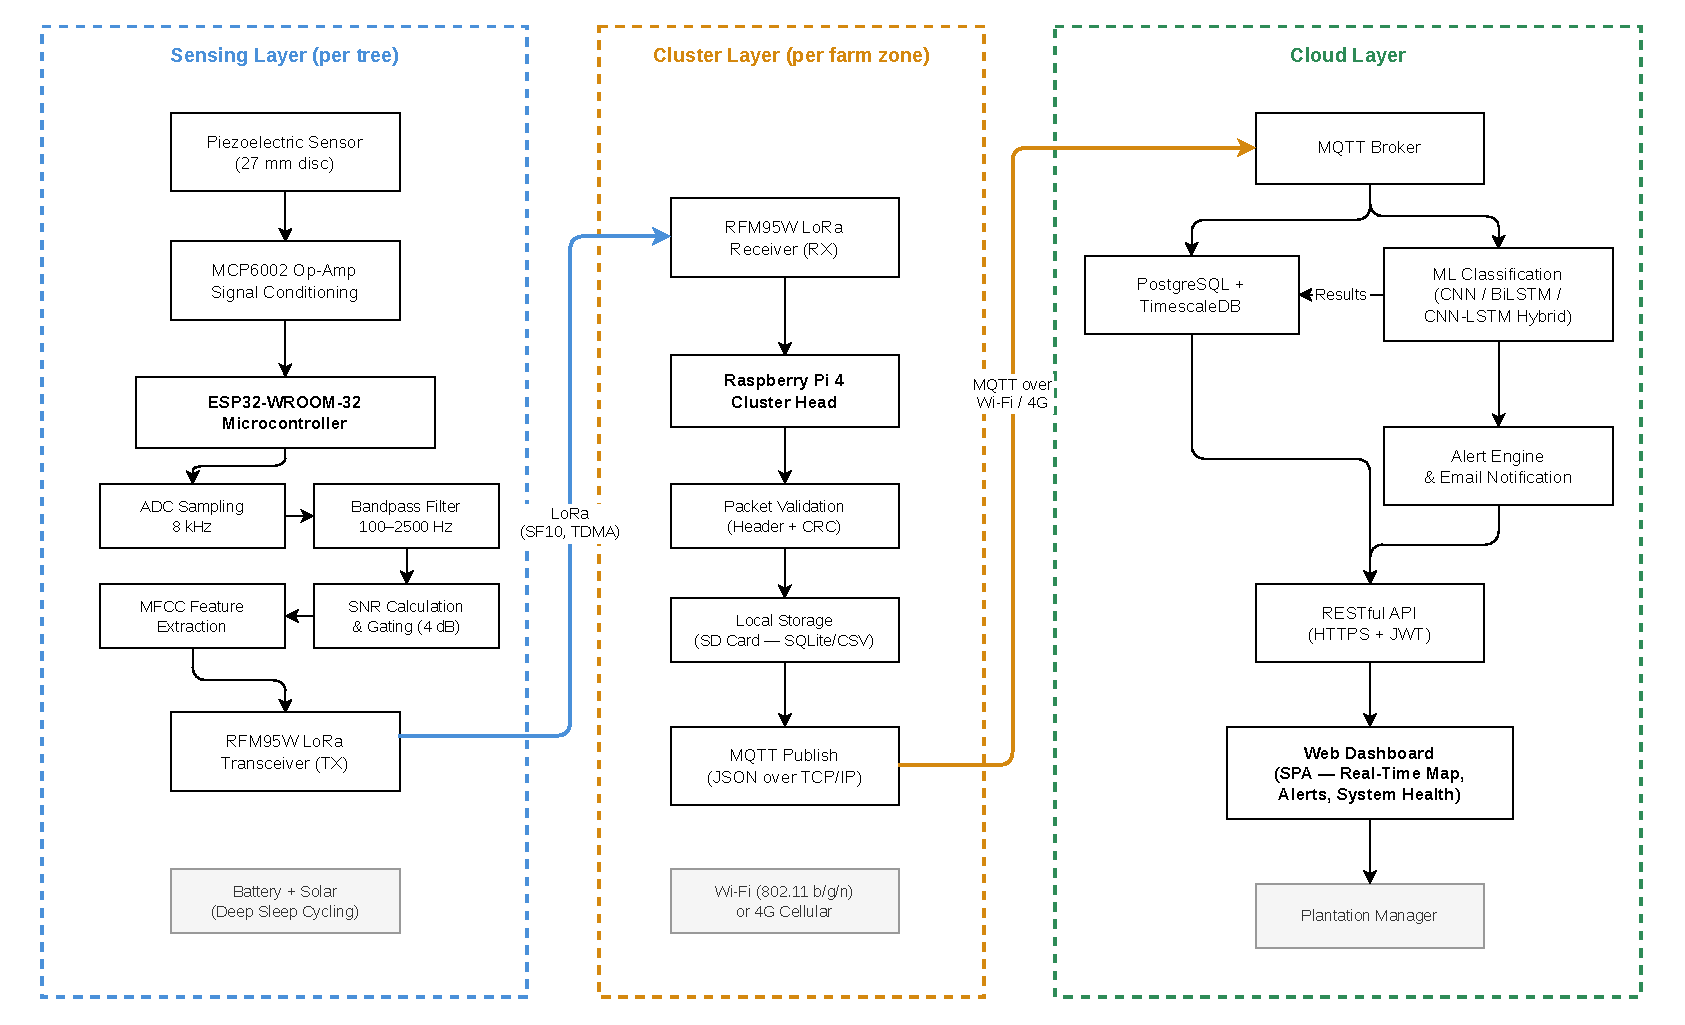
\includegraphics[width=1\textwidth]{figures/system_fig_diagram.pdf}
\caption{High-level block diagram of the proposed RPW acoustic detection system}
\label{fig:HighLevelBlockDiagram}
\end{figure}

\subsection{Sensing Layer}

The Sensing Layer is the field-deployed layer of the system. Each sensing node is composed of a piezoelectric disc sensor mechanically coupled to the surface of a palm trunk, an op-amp for analog signal conditioning, an ESP32 microcontroller for digitization and on-node processing, and a LoRa transceiver for wireless transmission. The piezoelectric element translates the mechanical vibrations produced by feeding activity of larvae resident inside the trunk to low-amplitude analog voltage signals in the millivolt range. All signal processing is performed on the ESP32 before any data leaves the sensing node. No raw audio is transmitted; only the extracted MFCC vector, along with the node identifier and a UTC timestamp, is packaged into a LoRa payload and sent to the cluster layer. The sensing nodes operate on a duty-cycled schedule aligned with the biological activity patterns of RPW larvae. This schedule maximizes detection probability while reducing power consumption, allowing nodes to run on batteries for extended periods with optional solar charging.

\newrevision{For bench validation, the signal path is: RPW recording $\rightarrow$ amplifier $\rightarrow$ vibration exciter mechanically attached to wood or palm material $\rightarrow$ piezoelectric sensor $\rightarrow$ MCP6002 $\rightarrow$ ESP32 $\rightarrow$ filtering, MFCC extraction, and classification. The exciter injects vibration into the material; it is not used as a speaker in air. A reference piezoelectric sensor mounted near the exciter records the injected vibration, while the normal measurement sensor records the vibration remaining after propagation through the material.}

\newrevision{Testing begins with a wood plank. When suitable real palm material is available, it may be used as a later material stage; a palm-trunk-section stage is not required. The controlled variables are source-to-sensor distance, playback amplitude, and added background vibration/noise expressed as SNR. This phased setup makes it possible to identify whether a failure arises from injection, propagation, sensing, processing, or classification.}

\newrevision{The normal uplink will be compared with a compact binary feature packet containing a packet-format version, compact node and time metadata, quantized MFCC values, and only beneficial delta or run-length coding. The selected packet format must be justified by measured payload, airtime, packet loss, energy, ESP32 memory/runtime, and detection metrics.}

\subsection{Cluster Layer}

The Cluster Layer is the always-on aggregation and forwarding tier between the field-deployed sensing nodes and the cloud backend. Each cluster head consists of a Raspberry Pi 4 Model B equipped with an RFM95W LoRa receiver module interfaced via SPI. The cluster head runs continuously on mains electricity and remains in continuous receive mode, listening for incoming LoRa packets from sensing nodes.

Upon receiving a LoRa packet, the cluster head validates the packet header and CRC check-sum. \newrevision{Valid packets are parsed into the node identifier, timestamp, SNR, compact features, and any defined burst statistics.} The parsed data is written to local storage (SQLite on an SD card) as a buffer against connectivity interruptions. If an uplink connection is available, whether Wi-Fi (IEEE 802.11 b/g/n) or 4G cellular, the cluster head publishes the data to the cloud backend via MQTT over TCP/IP as a JSON-encoded payload. If the uplink is temporarily unavailable, the data is buffered locally and forwarded upon reconnection. The cluster head does not perform classification or inference; it only aggregates and forwards data.

For large plantations, multiple cluster heads are deployed in non-overlapping geographic zones, each assigned a unique block of node identifiers. No inter-cluster-head coordination is required; the system scales linearly by adding cluster heads.


\subsection{Cloud Layer}

The Cloud Layer provides centralized data storage, deep learning inference, alert generation, and a monitoring interface. The cloud backend receives MQTT messages from all cluster heads, routes them through a message broker, and stores the incoming MFCC feature data alongside node and cluster health metadata in a PostgreSQL database extended with TimescaleDB for time-series storage and querying. Incoming acoustic feature data is classified by a trained deep learning model, based on CNN, CNN-LSTM, or Mamba (SSM) architectures, to determine whether the acoustic signature corresponds to active larval feeding or environmental noise. When the classification confidence exceeds a predefined threshold, the system generates an alert, logs it in the alert database, and sends automated email notifications to registered plantation managers. The web-based monitoring dashboard is the primary user interface, providing real-time visualization of sensor nodes, detection events, and system health. The dashboard communicates with the cloud backend through a RESTful HTTP API secured with HTTPS (TLS 1.2 or later) and JWT authentication, so plantation data is accessible only to authorized users. It runs in any standard desktop or tablet browser with no installation required.

\section{Hardware Design}

The hardware architecture of the system is organized into two layers: the sensing node (deployed per tree) and the cluster head (deployed per farm zone), with data ultimately flowing to a cloud backend for classification and monitoring. Below is a detailed description of every component in the system.

\subsection{Piezoelectric Disc Sensor}

Each sensing node begins with a 27 mm piezoelectric disc (Murata 7BB-27-4L0 or equivalent) coupled to the palm trunk through the selected mounting method and metallic waveguide. The element converts mechanical vibration into a low-amplitude electrical signal. Contact coupling reduces exposure to airborne noise compared with an air microphone, but the drilled waveguide makes the proposed mounting method minimally invasive and does not eliminate wind, bird, or machinery interference \cite{pinhas2008,karar2022}.

\subsection{MCP6002 Op-Amp Signal Conditioning Circuit}

The raw output of the piezoelectric sensor is too weak to be sampled reliably by the microcontroller's ADC. An MCP6002 operational amplifier circuit amplifies and conditions the signal, bringing it into the 0 to 3.3 V input range expected by the ESP32. Protective components including 1N4148 clamping diodes, decoupling capacitors, and a voltage divider network ensure that voltage spikes do not damage the ADC input. This stage also contributes to the initial noise rejection by shaping the signal bandwidth before digital filtering takes place.

\subsection{ESP32 Microcontroller}

The ESP32 serves as the brain of the sensing node. It performs ADC sampling and executes the on-node signal processing pipeline described in Section 4.3.3. No raw audio ever leaves the node; only the pre-computed features are transmitted, which dramatically reduces bandwidth and power consumption. The ESP32 was selected for its low cost, integrated Wi-Fi (useful for bench testing), adequate ADC resolution, and broad community support through the Arduino ecosystem.

\subsection{LoRa Transceivers}

Wireless communication between the sensing node and cluster head uses an RFM95W connected to the ESP32 through SPI. The prototype will configure an authorized local sub-band and test SF7 as an initial setting. Range and hourly capacity depend on payload airtime, permitted duty cycle, interference, antenna placement, and plantation conditions; the earlier 1 km and 8,000-transmission values are planning estimates that require measurement. Transmission scheduling and payload composition are described in Section 4.3.3.

\subsection{LoRa Antenna}

\newrevision{Both the sensing node and the cluster head use external antennas that match the selected deployment-region frequency plan. An external antenna, rather than an onboard PCB trace antenna, is intended to reduce attenuation from the enclosure and trunk.}

\subsection{Raspberry Pi 4 Model B}

The cluster head runs on a Raspberry Pi 4 with 4 GB RAM, powered continuously by a standard power outlet. It receives incoming LoRa packets from all sensing nodes in its zone via a second RFM95W LoRa module connected over SPI, logs each received MFCC feature packet to a local 32 GB SD card for redundancy, and forwards the data to the cloud backend over Wi-Fi (IEEE 802.11 b/g/n) or, where Wi-Fi is unavailable, data will be stored in a buffer until uplink is available. The cluster head does not perform any classification; it functions purely as an always-on aggregation and forwarding layer. The Raspberry Pi OS (Debian-based, 64-bit) runs a Python 3.10 daemon that handles packet reception, local logging, and MQTT publishing.

\subsection{Casing \& Optional Solar Panel}

\newrevision{Each node is designed for an enclosure targeting IP65 protection and may use a solar panel with battery regulation for autonomous outdoor operation. The prototype will not claim formal IP65 compliance until the enclosure is tested.}


\section{Software Design}

This section presents the software design of the RPW acoustic detection system. It covers the overall system architecture, the data architecture underlying persistent storage and data flow, and the detailed design of both static and dynamic system behaviors. Each diagram included in this section is discussed in the accompanying text.



\subsection{System Architecture}

A detailed description of the overall physical architecture of the application is presented in this section.

\subsubsection{Node Architecture}

The IoT-based RPW acoustic detection system is organized into a three-tier physical architecture comprising (1) the sensing node layer, (2) the cluster head aggregation layer, and (3) the cloud backend and dashboard layer. Each tier has clearly defined responsibilities and communicates with adjacent tiers through well-specified interfaces, enabling modular development, independent scaling, and fault isolation across the deployed network.

\paragraph{Sensing Node Layer} 

At the lowest tier, each sensing node uses the hardware described in Section 4.2: a piezoelectric disc sensor coupled to the palm trunk, an MCP6002 op-amp conditioning circuit, an ESP32-WROOM-32 microcontroller, and an RFM95W LoRa transceiver. The piezoelectric element converts internal mechanical vibrations generated by RPW larval feeding into a low-amplitude analog voltage signal, which is conditioned by the op-amp circuit before being digitized by the ESP32's onboard ADC at a sampling rate of at least 8 kHz, which satisfies the Nyquist criterion for the larval acoustic band of 100--2500 Hz. Once sampled, the ESP32 firmware applies a digital bandpass filter (100--2500 Hz), squares the filtered signal, computes a moving average to produce a power envelope, and calculates the Signal-to-Noise Ratio (SNR) of each measurement window. A transmission event is generated only when the SNR exceeds a 4 dB threshold, ensuring that bandwidth and energy are consumed only for acoustically significant events. \newrevision{When triggered, the node will compare a baseline MFCC representation with one or more compact formats. The selected format will contain a version field and measured metadata/feature encoding; its bytes and airtime will be reported for the chosen regional radio settings. For bench validation, a recording is amplified and applied through a vibration exciter mechanically attached to the test material. A reference piezoelectric sensor near the exciter measures the injected vibration, while the sensing sensor measures the vibration after propagation through the material.} No raw audio is ever transmitted across the network. Transmissions are coordinated using a Time Division Multiple Access (TDMA) scheme with 900 ms time slots distributed across two biologically informed windows: night-time (22:00--06:00, hourly) and daytime (06:00--22:00, four-hour intervals). This schedule aligns monitoring frequency with periods of heightened larval acoustic activity.

\paragraph{Cluster Head Aggregation Layer}

The intermediate tier consists of one or more Raspberry Pi 4 cluster heads with RFM95W LoRa modules. A cluster head remains on mains power, listens during the defined transmission windows, and writes received packets to the 64 GB microSD card included with the starter kit before forwarding them to the cloud through MQTT over Wi-Fi or an available cellular backhaul. Each JSON message contains the node ID, UTC timestamp, SNR, a quantized MFCC representation with its scale factor, and the defined burst statistics. The cluster head performs aggregation, local logging, and forwarding only. Additional cluster heads can divide a plantation into zones, but the supported coverage and node count will be based on prototype measurements rather than the earlier unvalidated 1 km and 8,000-node estimates.

\paragraph{Cloud Backend and Dashboard Layer}

At the top tier, a Linux-based cloud server (Ubuntu 22.04 LTS) receives all MQTT messages via a cloud MQTT broker and routes them through an automated preprocessing pipeline implemented in Python 3.10. Incoming MFCC feature vectors are validated, normalized, and passed to a trained deep learning inference service, which classifies each acoustic event as either RPW larval activity or ambient noise. Classification results, confidence scores, raw MFCC features, and node health telemetry are stored in a PostgreSQL database extended with TimescaleDB, which provides automatic time-based partitioning and accelerated range-query performance for the continuous time-stamped data streams. When a classification result exceeds a predefined confidence threshold, the alert engine automatically dispatches an email notification to registered plantation managers, identifying the affected node ID, farm zone, and detection confidence. A RESTful HTTP API (HTTPS, port 443, JWT-authenticated) exposes sensor status, historical feature records, classification results, and alert logs to the web-based monitoring dashboard. The single-page dashboard application provides real-time visualization of sensor node and cluster head locations on a map with color-coded infestation status markers, time-series graphs of acoustic energy levels per node, detection event timestamps with confidence scores, and system health indicators including battery levels and connectivity status for all nodes in the network.

\subsubsection{Node Topology}

The node architecture adopted for this system is a two-level hierarchical wireless sensor network (WSN). Sensing nodes communicate exclusively with their designated cluster head using LoRa (long-range, low-power) radio in a frequency plan selected for the deployment region. This star-of-stars topology was selected over a flat single-hop topology because it concentrates the energy cost of long-distance transmission at the always-on, mains-powered cluster head rather than at battery-constrained sensing nodes, and over a mesh topology because it eliminates the protocol overhead and latency introduced by multi-hop routing while still achieving the required plantation-wide coverage. The cluster head then forwards aggregated data to the cloud over a high-bandwidth backhaul (Wi-Fi or 4G), entirely decoupling the constrained sensing layer from the cloud infrastructure. \newrevision{The node-to-cluster link is a direct LoRa link; it shall not be described as LoRaWAN compliant unless LoRaWAN network and MAC components are added.} This architecture is illustrated conceptually in Figure 4.2 below.


\begin{figure}[h]
\centering
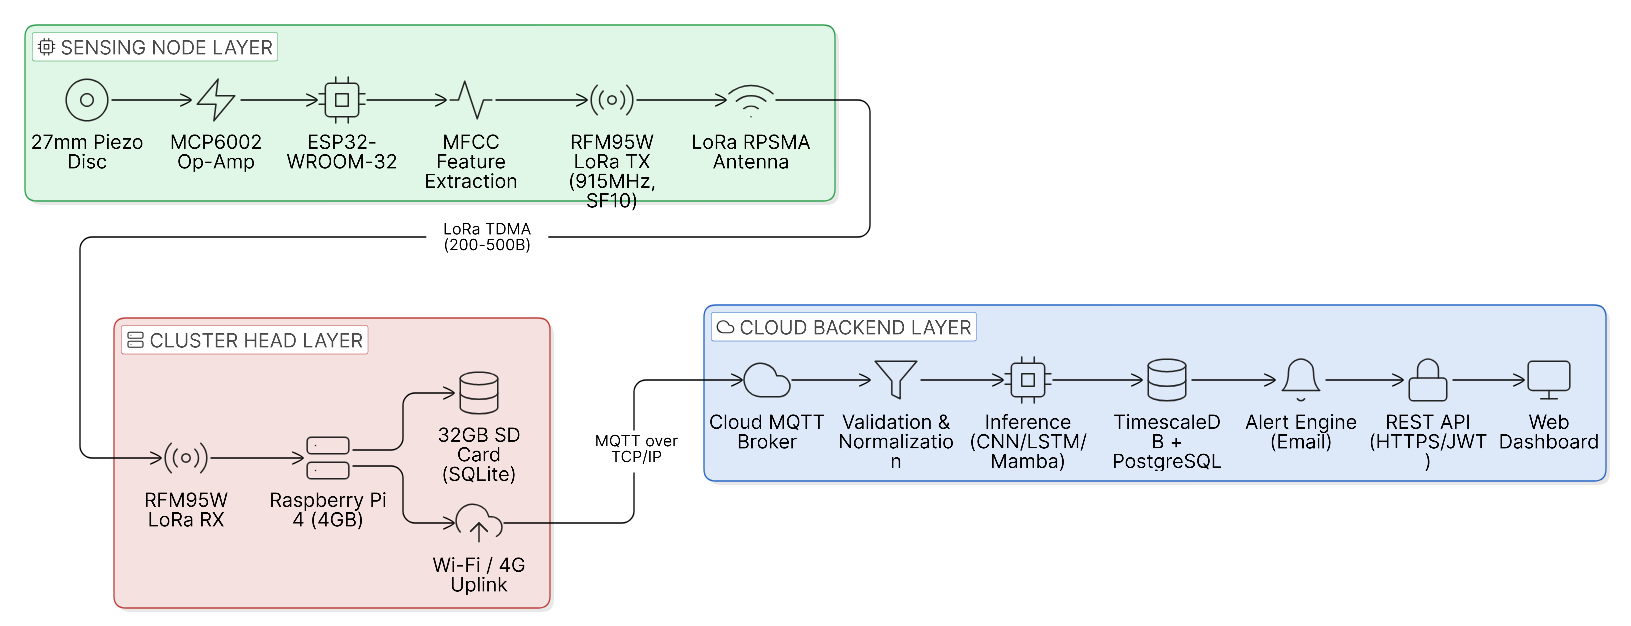
\includegraphics[width=0.95\textwidth]{figures/3Node_Arch.png}
\caption{Three-Tier Node Architecture of the IoT-Based RPW Acoustic Detection System}
\label{fig:ThreeTierNodeArchitecture}
\end{figure}


\subsubsection{Component Architecture}

Each tier of the system is composed of several internal software components that handle distinct stages of the detection pipeline. This section describes the responsibilities of each component and how they are organized within their respective nodes.

\paragraph{Sensing Node}

The sleep manager governs the ESP32's deep sleep and wake cycle, triggering wake-ups at the intervals defined by the active transmission window and returning the MCU to low-power mode after each recording and processing cycle completes. The ADC component captures a fixed-duration audio sample from the conditioned piezoelectric input each time the node wakes, buffering it in memory for downstream processing. The signal processing module runs the full on-device analysis pipeline, from bandpass filtering through power envelope computation and SNR evaluation to MFCC extraction, and makes the transmit-or-discard decision based on the SNR outcome. The LoRa transmitter handles payload assembly, TDMA slot timing, and packet dispatch through the RFM95W module. The power manager monitors battery voltage, manages solar charging state, and embeds a low-battery flag in outgoing packets when the node is approaching depletion so that operators can schedule maintenance before data loss occurs.

\paragraph{Cluster Head}

The LoRa listener is a continuously running daemon that receives incoming packets from sensing nodes, validates packet headers and CRC checksums, and discards malformed transmissions before passing valid data to the next stage. The storage component writes every validated packet to the local SD card as a timestamped entry, acting as a persistent buffer that retains data independently of uplink availability. The MQTT publisher reads from this buffer and forwards packets to the cloud broker whenever connectivity is present, automatically retransmitting any entries that were held during a connectivity interruption. The health manager periodically collects system-level diagnostics, including SD card free space, daemon uptime, and average RSSI across connected sensing nodes, and publishes them alongside the acoustic data so that infrastructure health is visible through the dashboard.

\paragraph{Cloud Backend}

The MQTT broker receives all incoming messages from cluster heads and routes them into the processing pipeline. The preprocessing service validates and normalizes incoming MFCC feature vectors before passing them to the inference engine. The inference engine loads the trained deep learning model and classifies each acoustic event, producing a label and a confidence score that are written to the database alongside the original features. The alert engine monitors classification outputs and, when the confidence score exceeds the configured threshold, generates a log entry and dispatches an email notification identifying the affected node and farm zone. The REST API serves stored data, including sensor status, classification history, and alert logs, to authenticated clients over HTTPS. The dashboard frontend consumes the API and renders the monitoring interface, providing the real-time map view, time-series graphs, detection event logs, and system health indicators that plantation managers interact with.

\subsubsection{Class Architecture and Static Representation}

The class architecture consists of 4 classes: ClusterHead, SensingNode, SensorMeasurement, and Tree. The ClusterHead and SensingNode classes represent the hardware components of Cluster Head and Sensing Node. Each ClusterHead can have many Sensing nodes connected to it, and each SensingNode can be connected to one ClusterHead. This relationship is represented by a bidirectional aggregation association relationship.


\begin{figure}[h]
\centering
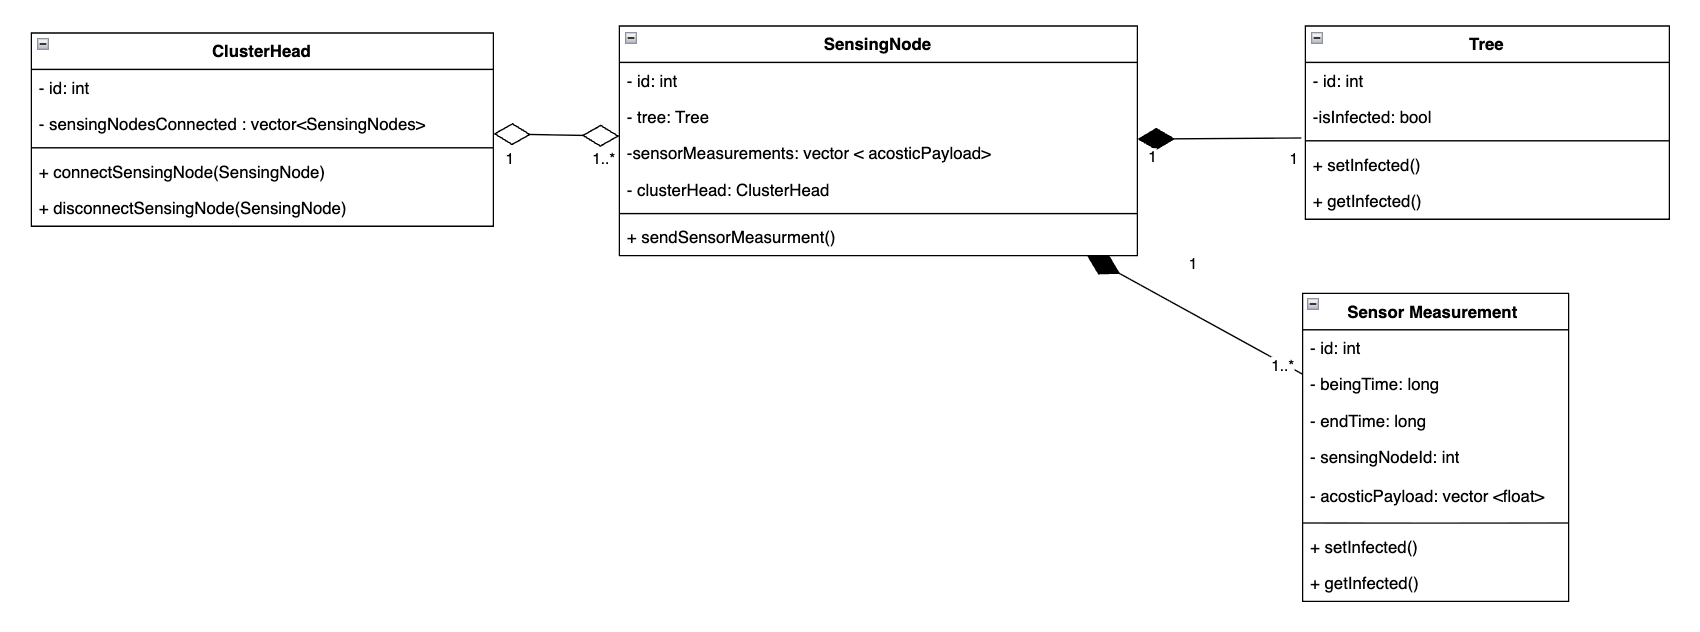
\includegraphics[width=1\textwidth,height=1\textheight,keepaspectratio]{uploads/Class Daigram.png}
\caption{Class architecture diagram of the RPW detection system}
\label{fig:ClassArchitectureDiagram}
\end{figure}

The SensorMeasurement class represents one “Chunk” of acoustic measurements, with a start time stamp, end time stamp, and an acoustic payload. Each SensingNode can have many SensorMeasurement stored in a dynamic array (vector). Each SensorMeasurement can only belong to one SensingNode. This is represented by a 1 to many composition relationship, because without a SensingNode no SensorMeasurement can be made. Each SensingNode is also associated with one tree, and each tree is associated with one sensing node, this relationship is represented by a one-to-one composition association, because without a SensingNode we cannot monitor a tree, and therefore for a tree to exist in our system it must be associated with exactly one sensing node.

\subsection{Data Architecture}

The data architecture is built on PostgreSQL extended with TimescaleDB. PostgreSQL provides a relational database engine supporting complex queries via standard SQL, while TimescaleDB adds automatic time-based partitioning (hypertables) and range-query performance suited to the continuous timestamped MFCC feature streams produced by the sensing layer. Together, they manage all relational data, cluster head and node metadata, time-series acoustic features, classification results, and user accounts, within a single database instance. The database schema consists of seven tables distributed across the three system layers. Figure 4.4 presents the ER diagram of the complete schema.

\subsubsection{Sensing Layer Tables}

The nodes table stores the registration record for each deployed sensing node, identified by a node id primary key (varchar). Each row contains the associated cluster id foreign key, the farm zone designation, geographic coordinates (location lat, location lon), and install date.

\begin{figure}[h]
\centering
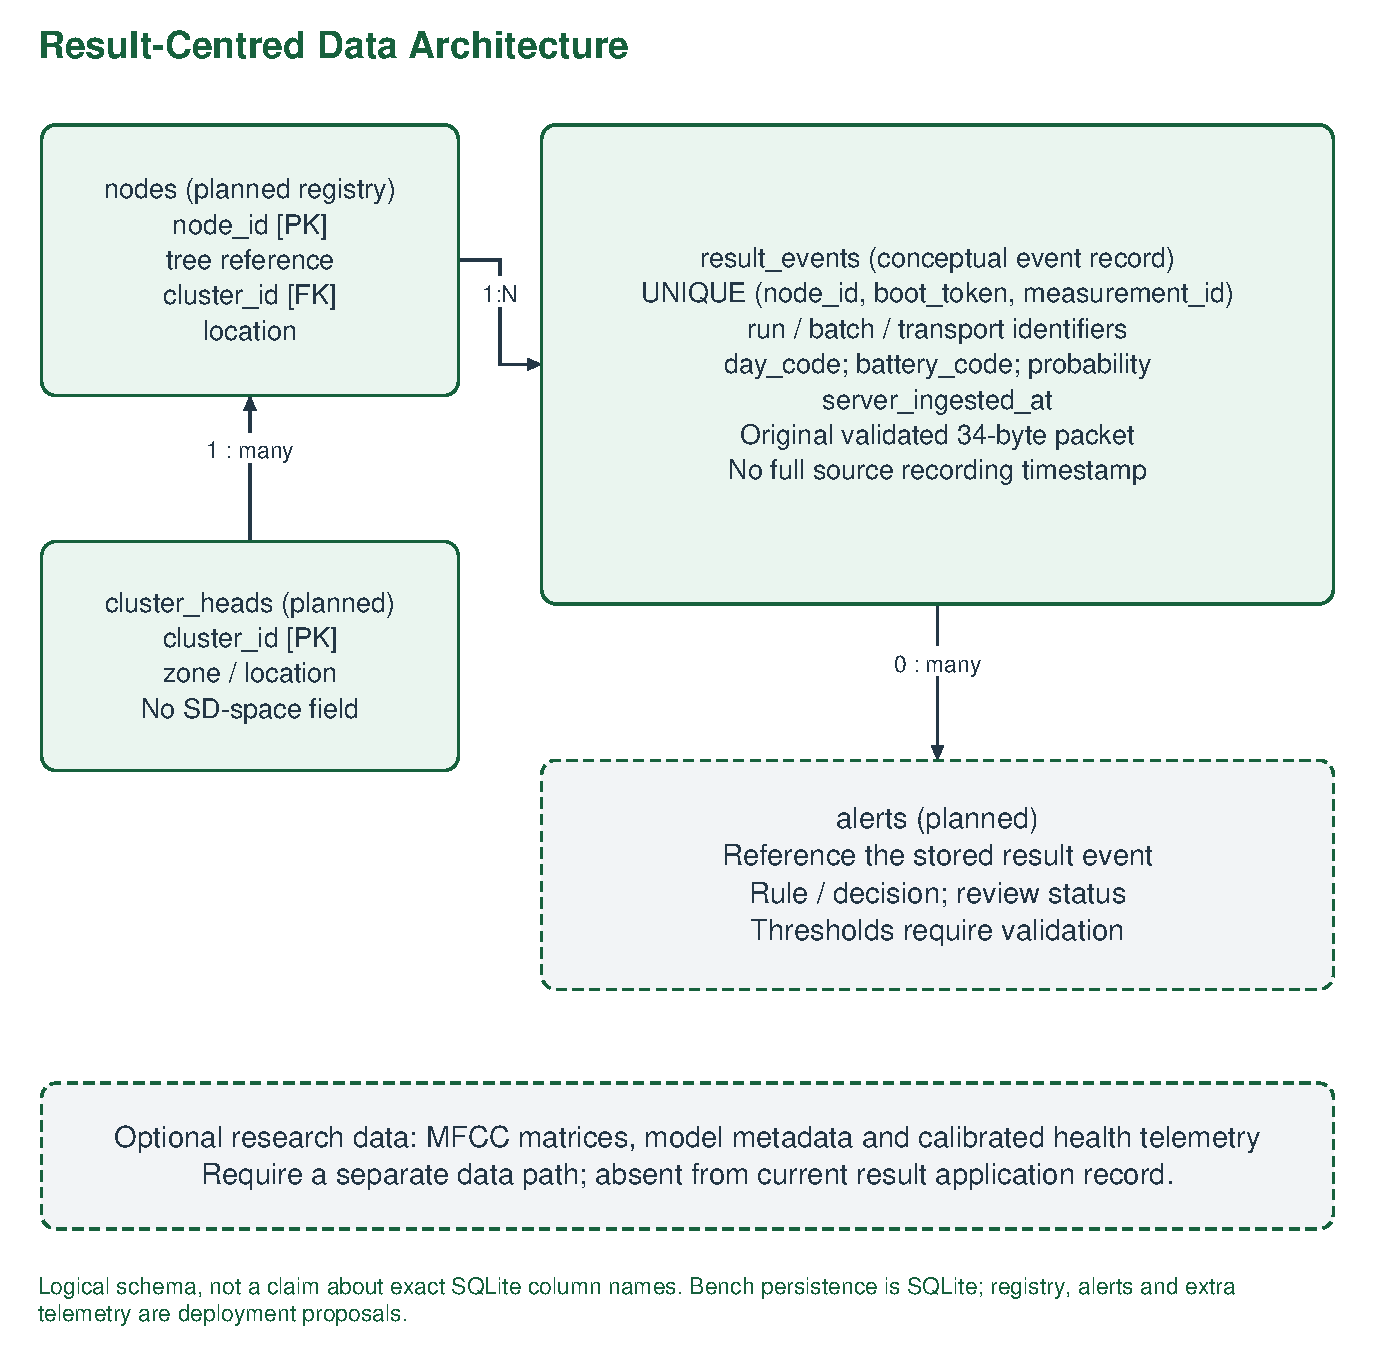
\includegraphics[width=0.95\textwidth]{figures/ER_Diagram.pdf}
\caption{Entity-Relationship diagram of the RPW detection system database}
\label{fig:EntityRelationshipDiagram}
\end{figure}

The relationship to cluster heads is one-to-many: each cluster head may have many sensing nodes, but each node belongs to exactly one cluster head. The node health hypertable records periodic health telemetry from each sensing node, indexed by a composite key of timestamp (timestamptz) and node id. Data columns include battery mv (millivolts), rssi dbm (dBm), and uptime s (seconds since last reset). Time-based partitioning keeps range queries efficient as the table accumulates months of deployment data. The acoustic features hypertable stores the preprocessed feature data transmitted by sensing nodes, indexed by timestamp and node id. The primary data column is mfcc (a 15×13 int8-quantized representation of the extracted MFCC vector), accompanied by snr db. Since feature extraction occurs entirely on the sensing node, no raw audio is stored. Records are retained for one year to support longitudinal infestation trend analysis.

\subsubsection{Cluster Layer Tables}

The cluster heads table stores static metadata for each deployed cluster head: cluster id, farm zone, geographic coordinates, install date, and uplink type (Wi-Fi or 4G cellular). It has a one-to-many relationship with both the nodes table and the cluster health hypertable. The cluster health hypertable logs periodic health telemetry from each cluster head, indexed by timestamp and cluster id. It records uptime s, rssi dbm, sd free mb (megabytes of remaining SD storage), and the current uplink type, allowing the dashboard to detect connectivity or storage issues before they cause data loss.

\subsubsection{Cloud Layer Tables}

The classification results hypertable stores the output of the deep learning inference pipeline, indexed by timestamp and node id. Each row contains the predicted label (e.g., ``infested'' or ``healthy''), the confidence score (0.0--1.0), and the model version identifier. Storing the model version with each result supports performance comparisons across model updates. The alert log hypertable records all detection alerts, indexed by timestamp and node id. Each row contains the alert type (e.g., ``infestation detected''), the classification confidence that triggered the alert, and an acknowledged flag indicating whether a plantation manager has reviewed it. Alert logs, along with the nodes and cluster heads metadata tables, are retained indefinitely.

\subsubsection{Data Retention and Partitioning Strategy}

The four hypertables are automatically partitioned by TimescaleDB along the timestamp dimension. Time-range queries, for example, retrieve all classification results for a specific farm zone over the past 30 days, executed against only the relevant partitions rather than the full table. Acoustic features and classification results are retained for one year, after which aged-out partitions are dropped automatically.

\subsection{Detailed Design}
\subsection{MFCC Quantization and Bounded Rice Compression}
\label{sec:mfcc_codec}
\newrevision{The packet-compaction design uses temporal delta encoding, zigzag mapping, and bounded Golomb--Rice coding. The supplied project codec notes describe a host benchmark and its reverse procedure. The receiving device in this project's updated architecture is an ESP32 cluster head. The same decoding procedure may run at the receiving endpoint or cloud, subject to implementation and resource testing. The notes' Raspberry Pi endpoint describes the earlier design.}

\begin{figure}[htbp]
\centering
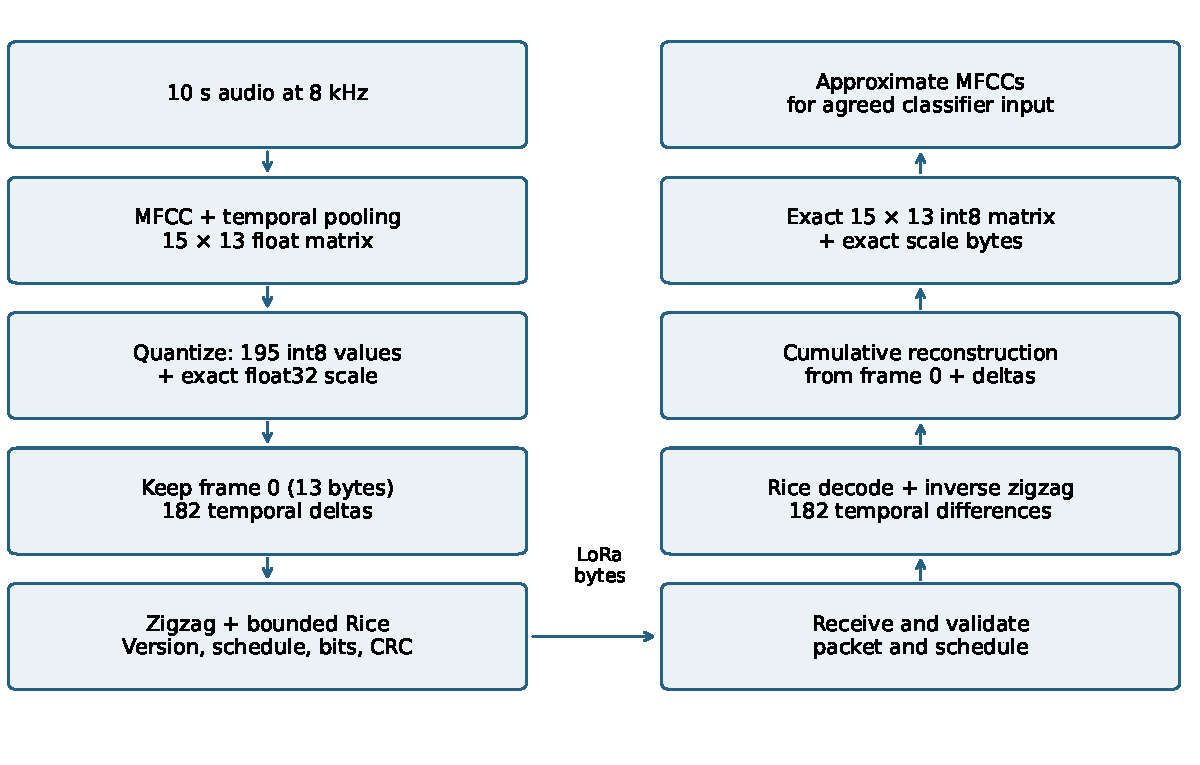
\includegraphics[width=\textwidth]{figures/mfcc_codec_pipeline.pdf}
\caption{\newrevision{MFCC encoding and reconstruction. The codec preserves the quantized matrix and scale exactly; audio and floating-point MFCC reconstruction remain lossy.}}
\label{fig:mfcc_codec}
\end{figure}

\begin{table}[htbp]
\centering
\caption{\newrevision{Reference MFCC extraction configuration supplied with the codec notes.}}
\label{tab:codec_frontend}
\begin{tabular}{p{0.28\textwidth}p{0.64\textwidth}}
\toprule
Stage & Configuration \\
\midrule
Input & Centre 10 seconds; stereo averaged to mono; shorter recordings excluded \\
Sampling & 8 kHz; 80,000 samples \\
Framing & 200-sample (25 ms) symmetric Hamming window; 80-sample (10 ms) hop; no end padding \\
Spectral transform & 256-point FFT power spectrum; 26 HTK-style mel filters over 0--4,000 Hz \\
Cepstral transform & Natural logarithm; orthonormal DCT-II; coefficients C0--C12 \\
Pooling & Average 998 complete frames in 15 consecutive groups; output $15\times13$ \\
Arithmetic & Float64 reference processing before quantization; one float32 scale \\
\bottomrule
\end{tabular}
\end{table}

\newrevision{The 15 output rows represent pooled time segments, rather than 15 original audio windows. This benchmark's 0--4,000 Hz mel configuration must be reconciled with the proposed 100--2,500 Hz node bandpass during frontend parity testing. Firmware and training must share windowing, pooling, normalization, rounding, and classifier input conventions. A codec round trip alone does not establish that parity.}

\newrevision{For floating-point matrix $M$, let $A=\max|M_{t,c}|$ and $s=\mathrm{float32}(A/127)$, using $s=1$ for an all-zero matrix. Quantization rounds $M_{t,c}/s$ to nearest even and clips to $[-127,127]$, producing 195 int8 values. The exact four scale bytes are retained. MFCC extraction, pooling, and quantization lose information relative to the recording; the subsequent codec is lossless relative to these integers and scale bytes. It cannot reconstruct the original WAV.}

\newrevision{The encoder stores all 13 values of the first pooled frame verbatim. For the remaining frames it computes $D_{t,c}=\mathrm{int16}(Q_{t,c})-\mathrm{int16}(Q_{t-1,c})$, yielding 182 temporal differences in time-major order. Subtraction uses at least 16-bit arithmetic to prevent overflow. For example, $[40,42,43,43,44]$ becomes an initial value of 40 and differences $[2,1,0,1]$; cumulative addition recovers the original sequence. Adjacent coefficients within a frame are never subtracted.}

\newrevision{Zigzag mapping converts each difference to $u=2d$ for $d\geq0$ and $u=-2d-1$ otherwise. With coefficient parameter $k_c\in\{0,\ldots,7\}$, the encoder computes $q=\lfloor u/2^{k_c}\rfloor$ and $r=u\bmod2^{k_c}$. If $q<15$, it writes $q$ one bits, a zero terminator, and exactly $k_c$ remainder bits. Otherwise it writes 15 one bits followed by the 9-bit literal $u$, without a terminator or remainder. This bounds a delta code at 24 bits. The generic int8 difference range is $[-255,255]$; the specified quantizer's $[-127,127]$ outputs give the narrower $[-254,254]$ range. Both fit the escape representation.}

\newrevision{For $k=0$, differences $[0,-1,+1,+2]$ encode as $0\,|\,10\,|\,110\,|\,11110$. Concatenating and padding these 11 meaningful bits gives bytes \texttt{0x5B 0xC0} in most-significant-bit-first order. The decoder uses the meaningful bit count and expected symbol count to distinguish information from zero padding.}

\begin{table}[htbp]
\centering
\caption{\newrevision{Rice schedule alternatives and experimental packet overhead.}}
\begin{tabular}{p{0.21\textwidth}p{0.39\textwidth}p{0.31\textwidth}}
\toprule
Method & Schedule choice & Decoder information \\
\midrule
Fixed & One trained 13-parameter vector & Matching provisioned version \\
Per packet & Best parameter for each coefficient in this recording & 39 descriptor bits, padded to 5 bytes \\
Predefined bank & Small trained bank; select the shortest candidate & Versioned registry and selector; benchmark charged selector within header flags \\
\bottomrule
\end{tabular}
\end{table}

\newrevision{A coefficient's parameter applies to its 14 differences throughout a packet. This is schedule selection, rather than parameter adaptation after every symbol. The experimental raw reference is 209 bytes: 195 feature bytes plus a 14-byte envelope that already includes the four-byte scale. Compressed packets contain that envelope, the 13-byte first frame, any schedule descriptor, and the byte-padded delta stream. A raw fallback is available when compression is larger. Final node ID, timestamp, application headers, and radio framing must be budgeted separately unless the chosen protocol explicitly includes them. The older example envelope offsets in the notes are not a verified specification of the newer benchmark. Firmware interoperability still requires its actual wire-format definition, schedule registry, and golden vectors.}

\newrevision{The receiver validates the mode, length, version, integrity check, finite positive scale, schedule identity, meaningful bit count, and padding. It reconstructs exactly 182 symbols using $c=i\bmod13$, reverses zigzag, and adds each difference to the same coefficient in the previous time frame. It rejects truncated codes, invalid escapes, out-of-range reconstructed values, and unexpected remaining bits. The result is the original quantized $15\times13$ matrix and exact scale bits. Optional dequantization gives $\widehat M=sQ$ under the classifier's agreed arithmetic.}

\subsubsection{Reported Host Compression Benchmark}
\newrevision{The supplied notes report the complete experimental packet sizes in Table~\ref{tab:codec_results}. Raw benchmark records and sample counts were not supplied with the explanation, so these values are reported project results awaiting reproduction. They provide no classification, measured radio airtime, or ESP32 runtime evidence.}

\begin{table}[htbp]
\centering
\caption{\newrevision{Reported held-out packet sizes for the validation-selected schedule bank.}}
\label{tab:codec_results}
\begin{tabular}{lrrr}
\toprule
Dataset & Mean bytes & p99 bytes & Mean reduction vs. 209 bytes \\
\midrule
LAB & 59.68 & 65 & 71.4\% \\
FIELD & 80.40 & 103 & 61.5\% \\
FARM-LIKE proxy & 72.16 & 98 & 65.5\% \\
\bottomrule
\end{tabular}
\end{table}

\begin{figure}[htbp]
\centering
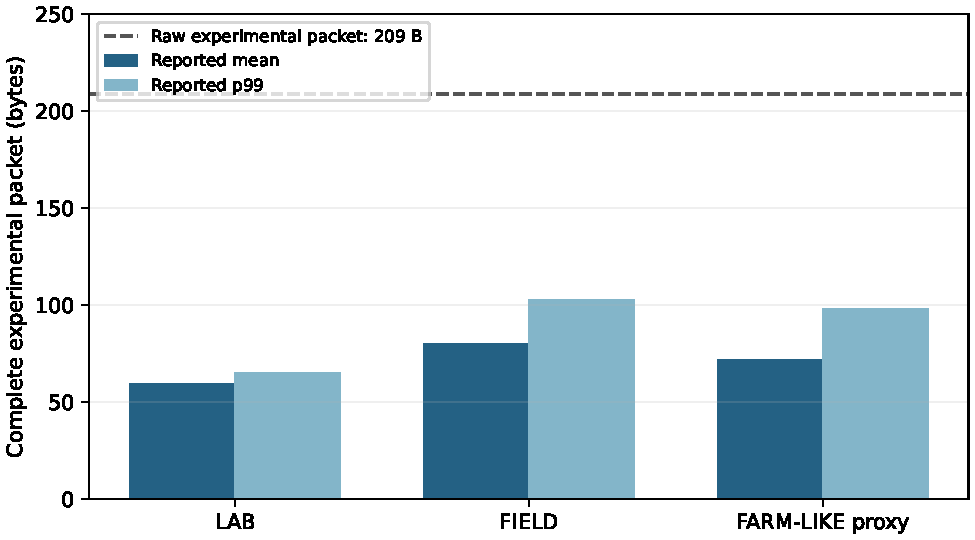
\includegraphics[width=0.93\textwidth]{figures/mfcc_packet_comparison.pdf}
\caption{\newrevision{Reported experimental packet sizes. Each dataset used a different trained schedule model. The FARM-LIKE proxy overlaps FIELD and is not confirmed date-palm-farm data.}}
\label{fig:codec_sizes}
\end{figure}
\newrevision{Verification will include byte-for-byte round trips of zero, alternating-sign, extreme-int8, and random matrices, followed by shared golden packet vectors. Payload reduction will be evaluated separately from packet delivery, energy, frontend parity, and detection performance.}
\FloatBarrier


\subsubsection{Dynamic Representation}

The dynamic behavior of the system is described through two operational flowcharts: the Sensing Layer flowchart (Figure 4.5), which details the on-node signal acquisition, processing, and transmission cycle; and the Cluster Layer flowchart (Figure 4.6), which describes the packet reception, validation, buffering, and forwarding logic at each cluster head.

\paragraph{Sensing Layer Operational Flow}

\begin{figure}[H]
\centering
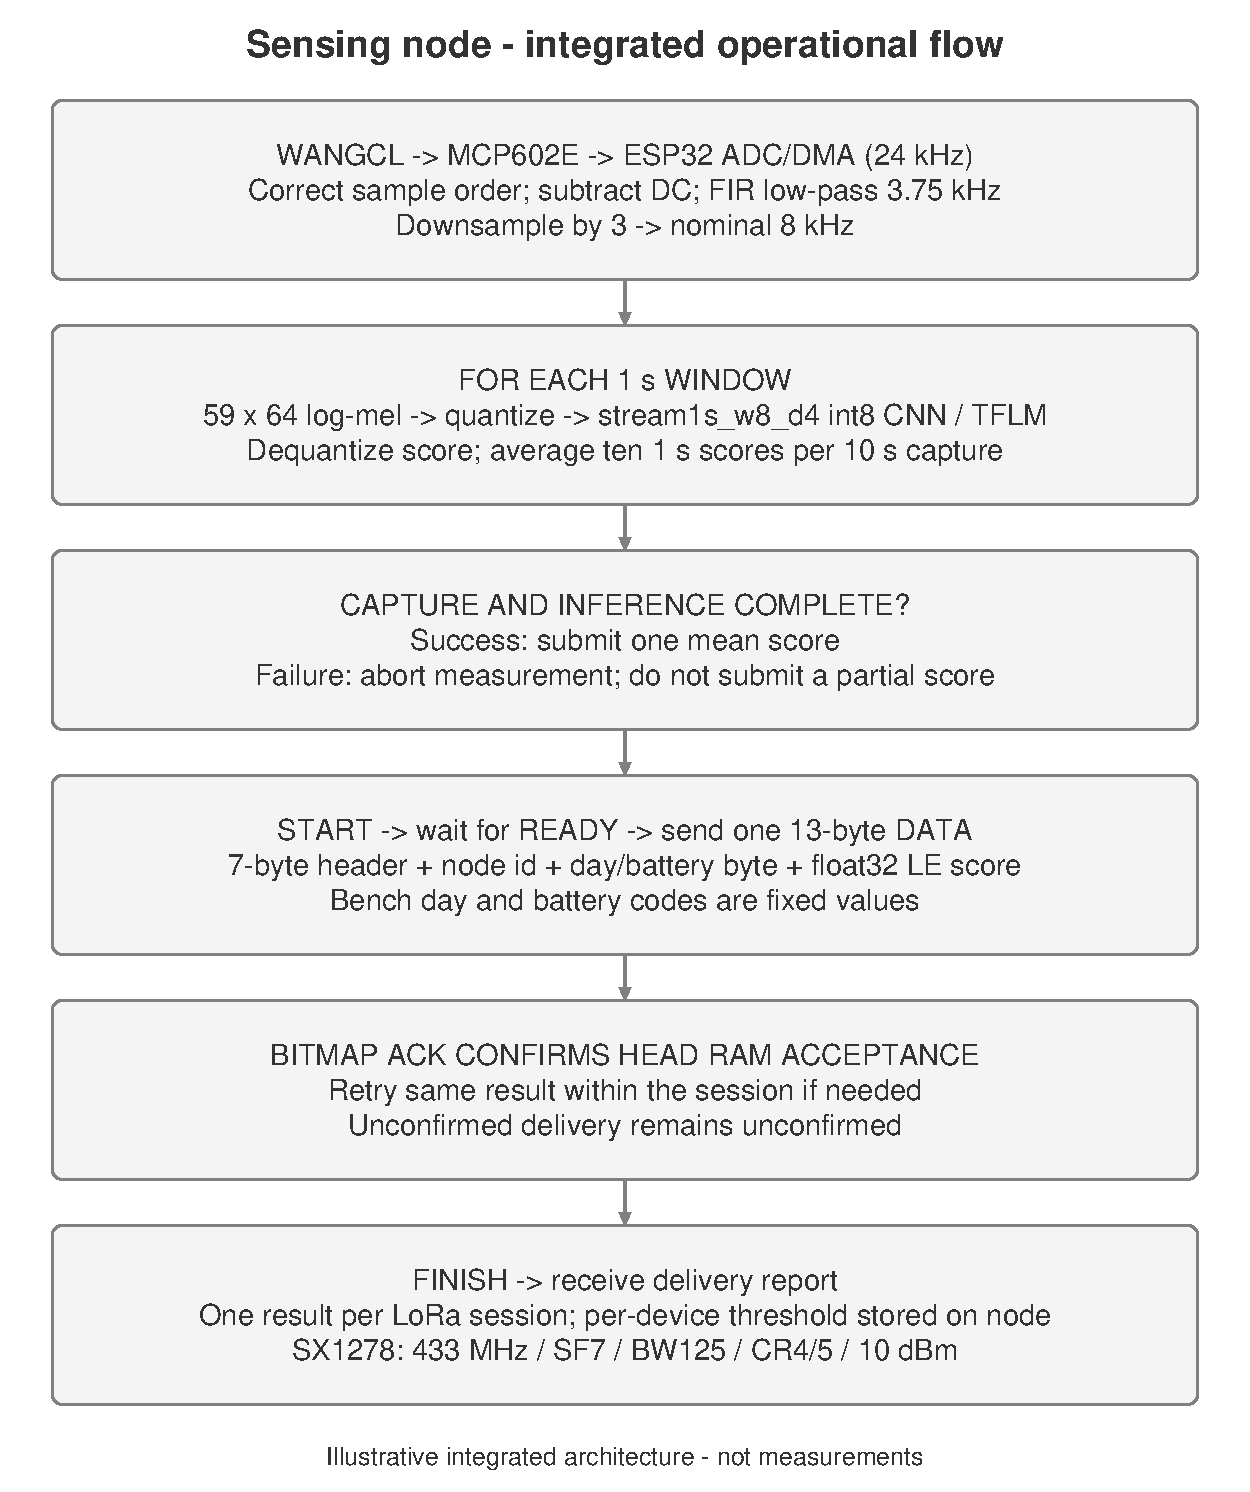
\includegraphics[width=0.88\textwidth,height=0.72\textheight,keepaspectratio]{figures/Sensing_layer_flowchart.pdf}
\caption{Sensing Layer operational flowchart}
\label{fig:SensingLayerFlowchart}
\vspace{0.5\baselineskip}
\end{figure}
\FloatBarrier

Figure \ref{fig:SensingLayerFlowchart} illustrates the complete duty cycle of the sensing node. The recorded signal is passed through a digital bandpass filter (100--2500 Hz) to suppress low-frequency environmental noise such as wind and ground vibrations, as well as high-frequency electronic noise above the band of interest. The filtered signal is squared element-wise to produce a strictly positive power envelope, and a 100 ms moving average is applied to smooth instantaneous noise spikes and reveal the temporal pattern of any larval feeding activity. This processing exploits the characteristic intermittent feeding behavior of RPW larvae, which produces distinct amplitude modulation in the moving average output when larvae are present, in contrast to the relatively flat output from healthy trees \cite{wang2021}. 

An SNR is calculated from the high-level and low-level values of the moving average output. This SNR definition is chosen to avoid false alarms from instantaneous noise spikes, which affect only brief portions of the recording window, while reliably detecting the sustained amplitude modulation characteristic of larval feeding. If the SNR exceeds the 4 dB decision threshold, the node extracts a fixed MFCC representation of 15 frames × 13 coefficients, quantized to int8 with a single global float32 scale factor. \newrevision{The project will serialize this information in a versioned packet and measure its byte length and airtime for the selected LoRa settings. Compact variants will be compared against the baseline rather than assigned a fixed size or airtime in advance. During bench validation, the reference trace, propagated-sensor trace, source-to-sensor distance, playback amplitude, and noise condition will be retained with each run.} After transmission, or if the SNR does not exceed the threshold, the node discards the recorded signal and returns to deep sleep. Under this SNR-gated transmission policy, most duty cycles in the absence of infestation produce no transmission, extending battery life and reserving network capacity for genuine detection events.

\paragraph{Cluster Layer Operational Flow}

\begin{figure}[H]
\centering
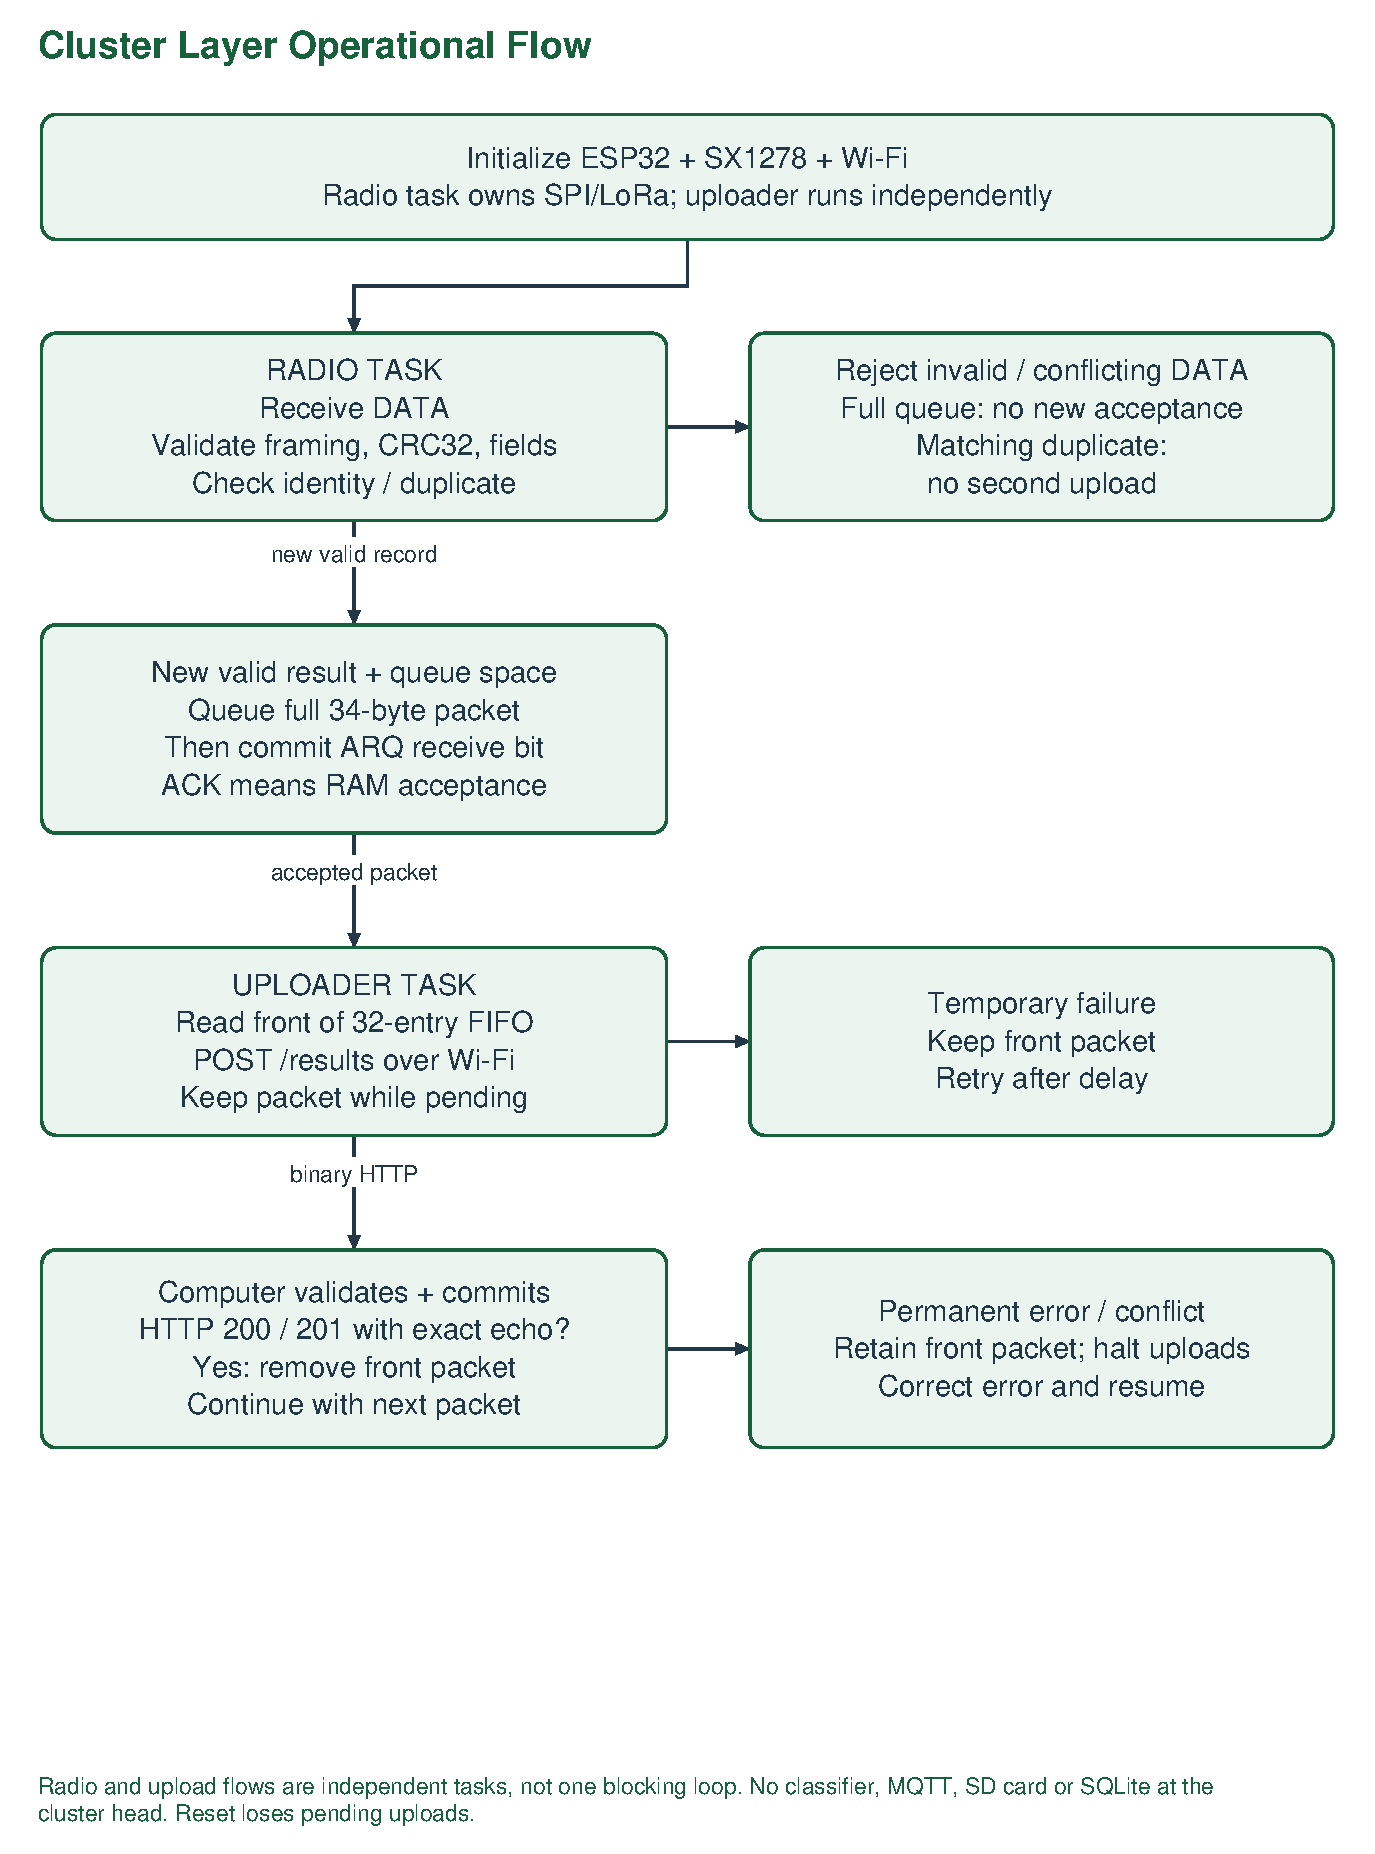
\includegraphics[width=0.88\textwidth,height=0.72\textheight,keepaspectratio]{figures/Cluster_layer_flowchart.pdf}
\caption{Cluster Layer operational flowchart}
\label{fig:ClusterLayerFlowchart}
\vspace{0.5\baselineskip}
\end{figure}
\FloatBarrier

Figure 4.6 illustrates the operational logic of a single cluster head. On boot, the Raspberry Pi 4 initializes the RFM95W LoRa receiver via SPI, configuring the operating frequency, spreading factor, and bandwidth to match the sensing node transmissions, then enters continuous receive mode.

When a packet arrives, the cluster head checks the header and CRC. Invalid packets, due to transmission corruption, collision, or interference, are discarded immediately. For valid packets, the cluster head parses the payload to extract the node identifier, UTC timestamp, MFCC feature vector, SNR value, and RSSI, then writes the data to local storage on the SD card in an SQLite format as a backup against upstream connectivity failures.

If an uplink connection is available (Wi-Fi or 4G cellular), the data is published to the cloud backend via MQTT as a JSON-encoded message containing the node identifier, timestamp, and MFCC feature vector. If the uplink is temporarily unavailable, the data is buffered locally and retried upon reconnection, implementing the store-and-forward strategy identified in the risk analysis (Section 7.7). After publishing or buffering, the cluster head resumes listening for the next packet.

\newrevision{The cluster head is a stateless relay. It carries out no classification or inference, passes the feature data through unmodified, and operates independently of all other cluster heads. Its supported node count will be determined from measured airtime, collision rate, packet loss, regional radio settings, and the selected payload format; no fixed capacity is claimed before those tests.}

\subsection{Classification Model Selection}
The cloud classifier is the final stage of the detection pipeline. Three candidate architectures will be trained on the same dataset and compared: a Convolutional Neural Network (CNN), a CNN-LSTM hybrid, and a Mamba-based selective state space model (SSM).

The CNN and CNN-LSTM architectures are established baselines in RPW acoustic detection and environmental sound classification (Section 2.5). Mamba is a recent selective state-space architecture \cite{gu2024mamba} that has not previously been applied to RPW acoustic data. Evaluating Mamba alongside the established CNN and CNN-LSTM baselines therefore constitutes a novel contribution of this project.

Because a missed infestation (false negative) allows larval damage to continue undetected and undermines the early-detection objective of this project, model selection prioritizes minimizing false negatives. The three candidate models are evaluated using:

Recall - the primary selection metric, quantifying the proportion of genuinely infested trees flagged by the system.

False Negative Rate (FNR) - the complement of recall, reported explicitly to highlight the proportion of missed infestations.

F1 score - the harmonic mean of precision and recall, used as a secondary metric to ensure that high recall is not achieved at the cost of unacceptably high false positive rates.

The candidate that maximizes recall while maintaining an acceptable F1 score will be selected for deployment. The deployed model can be updated over-the-air as new training data becomes available, without requiring physical access to any sensing node.

\section{Standards}

\subsection{Communication Standards}

\newrevision{The sensing-node to cluster-head link uses direct LoRa radio. Its frequency, output power, bandwidth, and duty-cycle settings shall be selected for the deployment region rather than fixed in advance. Cluster heads use available Wi-Fi or cellular backhaul. MQTT v3.1.1 (ISO/IEC 20922) carries messages from the cluster head to the cloud. The dashboard API uses HTTPS with TLS 1.2 or later and is compatible with HTTP/1.1 (RFC 9112).}


\subsection{Data and Encoding Standards}

\newrevision{The compact node-to-cluster packet includes a version field. MQTT and REST API JSON payloads conform to RFC 8259. All timestamps carried in payloads and database records use ISO 8601 UTC format.}

\subsection{Electrical and Safety Standards}

\newrevision{The sensing node and signal-conditioning circuit use low-voltage DC power. Any mains-powered cluster-head supply shall be certified for its intended use. IEC 62368-1 and relevant low-voltage DC practices guide the design; the prototype will not claim formal compliance without the required testing and certification.}

\subsection{Software and Coding Standards}

\newrevision{ESP32 firmware follows Arduino coding conventions, and Python backend code follows PEP 8 with linting. The API follows REST constraints, and JWT-based authentication follows RFC 7519.}

\subsection{Environmental Standards}

\newrevision{Outdoor enclosures target IP65 protection under IEC 60529. This is a design target; formal IP65 compliance requires an enclosure and test process that the prototype has not yet completed.}

\section{Alternative Design Approaches}

The proposed system architecture: low-cost piezoelectric trunk-mounted sensing nodes connected via LoRa to a cluster head that forwards MFCC features to a cloud-based deep learning classifier was selected after evaluating several alternative design approaches identified in the literature review. This section discusses the rationale for the chosen design relative to those alternatives.

\subsection{Invasive Probe-Based Piezoelectric Systems}

Conventional acoustic detection systems use piezoelectric probes inserted through drilled holes in the tree trunk to maximize acoustic coupling between the sensor and the internal wood structure \cite{pinhas2008,karar2022}. Such probe-based systems have demonstrated strong detection performance, including GMM/VQ-based classifiers achieving detection rates of up to 98.9\% in soundproofed laboratory conditions \cite{pinhas2008}. However, this invasive installation approach introduces entry points for secondary pests, pathogens, and fungal infections into each monitored tree, a risk that compounds with the number of sensing nodes deployed across a large plantation. Repeated trunk penetrations also present regulatory and agronomic concerns. The proposed system instead uses the piezoelectric disc in surface-contact mode, placed directly on the bark surface, eliminating the need for trunk penetration and reducing invasiveness while retaining adequate signal sensitivity within the 1.5-2.0 m effective radius documented in the literature \cite{pinhas2008,karar2022}.



\subsection{Non-Acoustic Detection Methodologies}

Three major non-acoustic detection methodologies were evaluated as potential alternatives or complements to acoustic sensing.

\subsubsection{Volatile Organic Compound (VOC) Biosensing}
Volatile Organic Compound (VOC) biosensing exploits infestation-specific metabolic byproducts that diffuse through palm tissue and can be detected externally without destructive sampling. While VOC sensing offers high specificity to larval metabolic activity, current implementations require genetically engineered bacterial biosensor panels and laboratory-grade plate reader equipment that are incompatible with continuous, autonomous field deployment across large plantations. The technology remains at the proof-of-concept stage for RPW detection and does not yet support the real-time, per-tree monitoring resolution required by this project.

\subsubsection{Molecular Marker Detection}
Molecular analysis can support species confirmation when suitable insect, frass, or tissue material has already been collected. The studies cited in this report did not validate low-level diagnosis from a living palm. Sampling and laboratory processing also make this approach unsuitable for the project's scheduled automated monitoring objective.

\subsubsection{Pheromone Trapping Systems}
Pheromone trapping systems capture dispersing adult weevils and provide spatial information about infestation hotspots. Although trap optimization studies have demonstrated effective adult capture rates in UAE and Saudi Arabia conditions, pheromone traps are inherently limited to detecting adult insects and yield no information about internal larval activity. Since structural damage to the palm tree occurs during the larval stage, reliance on adult capture alone cannot guarantee detection before irreversible internal damage has occurred, contradicting the early-detection objective of this project.

\subsubsection{Thermal Imaging and Remote Sensing}
Thermal imaging and remote sensing approaches attempt to measure physiological stress signals or internal fermentation heat associated with infestation. However, published accuracy levels for these methods are generally below 75\% in large-scale field assessments, and they are heavily susceptible to environmental noise from ambient temperature variation, making them unsuitable as a primary detection modality.

\subsection{Edge Classification vs. Cloud-Based Classification}

An alternative architectural choice considered was performing the full deep learning classification on the sensing node (edge inference) rather than transmitting features to the cloud. On-device inference using TinyML frameworks would eliminate latency associated with cloud communication and reduce bandwidth requirements to binary infestation/no-infestation flags. However, the CNN/CNN-LSTM hybrid architectures identified as the highest-performing classifiers for RPW detection impose memory and compute requirements that significantly exceed the capabilities of the ESP32 microcontroller (520 KB SRAM, dual-core at 240 MHz) when operating on full MFCC feature vectors. Furthermore, cloud-based inference allows the classification model to be updated over-the-air as new training data becomes available without requiring physical access to deployed sensing nodes, which is a significant operational advantage for large commercial plantations. The proposed design therefore adopts a hybrid strategy: lightweight signal processing, SNR-based gating, and MFCC feature extraction are performed on the ESP32 to drastically reduce the volume of data transmitted. Meanwhile, the computationally intensive deep learning inference is performed on cloud infrastructure with sufficient processing power. This division of labor respects the bandwidth constraints of LoRa and the hardware limits of embedded nodes, while preserving the classification accuracy achievable only with large-scale deep learning architectures.

\subsection{Wi-Fi-Only vs. LoRa-Based Wireless Communication}

\newrevision{A simpler network architecture using only Wi-Fi communication between sensing nodes and a local gateway was considered. Wi-Fi offers high bandwidth and low latency, but its coverage and power use can require denser gateway placement and more demanding node power design than LoRa. LoRa is appropriate for low-rate feature transmission, but its range, airtime, capacity, and energy consumption depend on the regional settings, payload, antenna placement, interference, and plantation conditions. The project will measure those properties for the selected configuration rather than claim a fixed range, payload size, or throughput in advance \cite{lorawan2023}.}


% ===============================
% CHAPTER 5: Implementation
% ===============================

\chapter{Implementation}
\label{ch:Implementation}

\section{Hardware Implementation}
\label{sec:HardwareImplementation}

Two physical layers are being implemented in the system, a sensing node placed on every tree and a cluster aggregation node per farm zone.

Each sensing node centers around the ESP32-WROOM-32, which handles ADC sampling, signal processing, and LoRa scheduling/transmission. A 27mm piezoelectric disk is mounted on the palm trunk directly to pick up vibrations from larval feeding. The raw output will be in millivolts, so an MCP6002 op-amp will be used to amplify the raw output into a window that the ESP32's ADC can use. \newrevision{A HopeRF RFM95W LoRa module, paired with an antenna matching the selected deployment-region frequency plan, handles transmission to the cluster head.} Nodes will run on battery with an optional solar charging circuit for longer deployments.

The cluster head is a Raspberry Pi 4 Model B with a second RFM95W for receiving packets. It connects out via Wi-Fi or 4G, runs on mains, and does no signal processing---its only job is to collect packets and forward them upstream.

Circuit schematics, assembly photographs, timing diagrams, and performance metrics (ADC fidelity, op-amp gain, LoRa link budget, power draw) will be documented in Senior Design 2 after bench testing.

\section{Software Implementation}
\label{sec:SoftwareImplementation}


\newrevision{The software design for this project consists of four main classes: Tree, SensingNode, SensorMeasurement, and ClusterHead. Each tree is associated with exactly one sensing node, and each sensing node is associated with exactly one tree. Each SensingNode should have many SensorMeasurement objects, accumulated over time. Each SensingNode is associated with one cluster head. The number of nodes per cluster head is a measured deployment result, not a fixed software assumption.}

A graphical user interface is planned to be developed, which is intended to be used by farms to view live RPW infestation predictions for each tree, as well as system health data such as node battery life and number of active nodes. 

To communicate between the cluster head and the cloud server,  MQTT broker with TCP/IP will be used. The cluster head should send MFCC vectors to the cloud server along with the most recent system health data. The system health data will be stored in a  system health table in the server hosted PostgresSQL database. A preprocessing pipeline running on the cloud server prepares the MFCC vectors for ML inference. ML inference should run on the cloud server.The ML inference results should be stored in a database hosted on the server. A server script should provide a RESTful API endpoint that allows  the front end of the web Dashboard  to connect with the cloud server., This will allow serving the most recent ML inference results and system health data from the results table and system health table in the PostgresSQL database. Farm employees can login in into the web dashboard through JWT authentication. An email alert system should also be implemented, which uses  SMTP to send automated email alerts to appropriate farm staff  once a predefined confidence threshold for a Tree's infestation is met.

\section{Integration and Deployment}
\label{sec:IntegrationDeployment}

Integration planning is complete, with physical deployment scheduled for Senior Design 2. During that phase, each hardware component will be assembled and validated individually before full system integration.

From the sensing node outward, the ESP32 captures a 10-second acoustic sample, applies bandpass filtering and SNR-based gating, extracts an MFCC feature vector, and transmits a compact payload via LoRa to the cluster head. Communication timing is managed using a TDMA scheme with 900 ms slots. Two transmission windows are defined to match larval activity patterns: nighttime (10 PM--6 AM, hourly) and daytime (6 AM--10 PM, every four hours).

At the cluster head, each valid packet is stored locally on an SD card and then forwarded as a JSON message over MQTT/TCP. In the cloud backend, the received features are processed through the inference pipeline, stored, and evaluated against a confidence threshold. If the threshold is exceeded, an email alert is triggered. A web dashboard provides the plantation manager with a real-time overview of system activity and status.

\newrevision{Physically, each sensing node is installed on a single tree trunk. For larger plantations, multiple cluster heads may be deployed in separate zones. Their radio range and supported node count will be reported from measured prototype conditions, including the selected spreading factor, payload, antenna placement, interference, and regional settings.}

Comprehensive integration testing, including multi-node operation, packet loss rates, end-to-end latency from signal capture to alert, and real-world field deployment, will be conducted and reported in Senior Design 2.

\section{User Interface Implementation}
\label{sec:UIImplementation}

The primary user interface for this project is the farm dashboard (prototype screens shown below). The main goal of this dashboard is to present the machine learning inference data in a manner that makes it possible for farms to gain insights on the infestation status of their palm trees. The top of the dashboard screen shows a live summary of the tree measurements, showing the number of trees being monitored, the number of trees suspected to have an infection, and the number of active nodes. Below this summary, the user can see live detailed data on each tree being monitored, with each tree indicated by a card. Further features that could be added to this dashboard are a tree map view, which shows each tree's geolocation on a satellite map, along with the tree's data, allowing farms to easily locate infested trees. Furthermore, each tree card in the main dashboard should have a navigate-to-tree feature, facilitating easy access to the tree's location in the farm.

\FloatBarrier

\begin{figure}[H]
    \centering
    \includegraphics[width=0.9\linewidth]{\detokenize{figures/WhatsApp Image 2026-04-17 at 09.31.17.jpeg}}
    \caption{Farm dashboard prototype - Sensor Map Screen.}
    \label{fig:dashboard_screen_sensormap}
\end{figure}

\begin{figure}[H]
    \centering
    \includegraphics[width=0.9\linewidth]{\detokenize{figures/WhatsApp Image 2026-04-17 at 09.31.17 (1).jpeg}}
    \caption{Farm dashboard prototype - Acoustic Analysis Screen.}
    \label{fig:dashboard_screen_acousticanalysis}
\end{figure}

\begin{figure}[H]
    \centering
    \includegraphics[width=0.9\linewidth]{\detokenize{figures/WhatsApp Image 2026-04-17 at 09.31.18.jpeg}}
    \caption{Farm dashboard prototype screen - Alert Log Screen.}
    \label{fig:dashboard_screen_alertlog}
\end{figure}

\begin{figure}[H]
    \centering
    \includegraphics[width=0.9\linewidth]{\detokenize{figures/WhatsApp Image 2026-04-17 at 09.31.18 (1).jpeg}}
    \caption{Farm dashboard prototype - Historical Records Screen.}
    \label{fig:dashboard_screen_historicalrecords}
\end{figure}

\begin{figure}[H]
    \centering
    \includegraphics[width=0.9\linewidth]{\detokenize{figures/WhatsApp Image 2026-04-17 at 09.31.18 (2).jpeg}}
    \caption{Farm dashboard prototype screen - System Health Screen.}
    \label{fig:dashboard_screen_systemhealth}
\end{figure}

\FloatBarrier

The dashboard prototype screens shown in Figures~\ref{fig:dashboard_screen_sensormap}--\ref{fig:dashboard_screen_systemhealth} were designed using Claude Sonnet 4.6 LLM, using the following prompt (Claude also had previous context about this project outside this prompt):

\begin{quote}
\textit{I am designing a web dashboard for farms to user, it should show stats such as number of trees currently being monitored, trees suspecteted to have infection and the confidence of that infection. It should show the number of nodes currently linked to the system, and the number of measurements we are currently getting. Under these dashboard stats, there should be a view of all trees currently being monitored, with each tree represented as a card, showing infection health of the tree, frequency at which measurements are being done, and the average model infestaton prediciton over last 3 runs. each tree id should be present on the card as well. for accents and ctas, use this green color : \#7CEA9C show  sensor status, historical feature records, classification results, and alert logs to the web-based monitoring dashboard. The single-page dashboard application provides real-time visualization of sensor node and cluster head locations on a map with color-coded infestation status markers, time-series graphs of acoustic energy levels per node, detection event timestamps with confidence scores, and system health indicators including battery levels and connectivity status for all nodes in the network., change the name of that application to be NAKHEL}
\end{quote}


% ===============================
% CHAPTER 6: Validation, Verification, and Performance Analysis
% ===============================

\chapter{Validation, Verification, and Performance Analysis}
\label{ch:Validation}

This section presents the planned approach for evaluating the proposed RPW detection system in Senior I. It describes how the system will be verified against its requirements, how it will be validated for the intended use case, and how its performance will be assessed once implementation is complete.

\section{Testing}
\label{sec:Testing}

Testing will be conducted using both white-box and black-box approaches, depending on the subsystem under evaluation. White-box testing will be used for internal components such as the sensing firmware, signal conditioning logic, feature extraction pipeline, and cloud-side processing modules. Black-box testing will be used for end-to-end system behavior, where input acoustic signals are applied and the resulting classification, transmission, and alert outputs are observed.

Test cases will be derived directly from the system requirements to ensure traceability. Each functional requirement will be mapped to one or more test cases so that the sensing node, wireless communication, classification model, database storage, and dashboard functions are all covered. The planned coverage will include normal operation, noisy acoustic conditions, and simulated infestation-like inputs.

\begin{table}[h]
\centering
\caption{Planned Test Cases by Requirement Area.}
\label{tab:testcases}
\renewcommand{\arraystretch}{1.3}
\begin{tabular}{@{} p{0.25\linewidth} p{0.38\linewidth} p{0.28\linewidth} @{}}
\toprule
\textbf{Requirement Area} & \textbf{Planned Test Focus} & \textbf{Expected Result} \\
\midrule
Sensor acquisition    & Verify acoustic sampling from the trunk-mounted sensor & Signal is captured correctly \\
Signal processing     & Verify filtering and feature extraction                & Noise is reduced and features are generated \\
Wireless transmission & Verify data transfer to the cluster or server          & Packet is received without major loss \\
Classification        & Verify model inference on acoustic input               & Infestation or non-infestation is predicted \\
Alert generation      & Verify notification logic                              & Alert is triggered when threshold is exceeded \\
Dashboard display     & Verify data visualization and status display           & Results appear correctly on the interface \\
\bottomrule
\end{tabular}
\end{table}

\newrevision{The controlled bench campaign will use the mechanical path above, not a free-air speaker test. For every distance, amplitude, and noise/SNR condition, the team will store the reference-sensor trace, measurement-sensor trace, received packet record, and classifier output. Playback fidelity will compare the injected reference with the intended signal; propagation will be summarized as SNR versus distance; detection will be summarized as recall versus distance and noise; and the classifier will report precision, recall, and F1.}

\section{Verification and Validation}
\label{sec:VandV}

Verification will confirm that the system is built according to the design specifications. This includes checking that the sensing node samples at the intended rate, that the signal is filtered within the target frequency range, and that the output data is transferred and stored in the correct format. Verification also includes confirming that the database structure supports the required records for sensor readings, classification results, and alerts.

\newrevision{Validation will first confirm that the bench apparatus can reproduce and measure controlled vibration through the selected material. This evidence is different from validation of live RPW detection. The project may claim live-detection evidence only after separately documented tests on naturally infested palms; otherwise it will report the work as emulation and bench validation. Since this is Senior I, the validation plan focuses on the method to be used rather than final experimental outcomes.}

\section{Simulation}
\label{sec:Simulation}

Simulation will be used to evaluate the design before field deployment. Acoustic signals representing healthy trees and infestation-like activity will be used to test the processing pipeline and classification flow. Simulated inputs will also help verify whether alerts are generated only when the confidence level or decision threshold is met.

A simulation-based evaluation will be carried out for the sensing, communication, and software layers. On the hardware side, artificial vibration or recorded signals can be used to mimic larval feeding activity. On the software side, labeled acoustic data can be used to test the classifier, database update logic, and dashboard behavior without requiring live plantation deployment.

\newrevision{The emulation setup uses recordings replayed through an amplifier and a mechanically attached vibration exciter. It is intentionally a controlled approximation when naturally infested palms are unavailable. The experiment will not be described as proof of field detection, and the playback, propagation, and classification measures will be reported separately.}

\begin{table}[h]
\centering
\caption{Planned Simulation Components.}
\label{tab:simulation}
\renewcommand{\arraystretch}{1.3}
\begin{tabular}{@{} p{0.28\linewidth} p{0.38\linewidth} p{0.25\linewidth} @{}}
\toprule
\textbf{Simulation Component} & \textbf{Input Type} & \textbf{Planned Purpose} \\
\midrule
Sensor node        & Synthetic vibration or recorded acoustic sample & Verify signal capture \\
Filtering stage    & Mixed-frequency audio input                     & Verify noise suppression \\
Feature extraction & Preprocessed acoustic clip                      & Verify feature generation \\
Classifier         & Labeled sample data                             & Verify prediction accuracy \\
Communication layer & Encoded event data                             & Verify packet transmission \\
Dashboard          & Stored detection event                          & Verify monitoring display \\
\bottomrule
\end{tabular}
\end{table}

\section{Performance Metrics}
\label{sec:PerformanceMetrics}

The system will be evaluated using metrics that reflect the objectives of the project. Accuracy will measure how well the classifier distinguishes infestation from non-infestation. Precision and recall will be used to understand false alarms and missed detections. Latency, packet loss, and uptime will be used to assess whether the system is suitable for continuous monitoring in a plantation environment.

\begin{table}[h]
\centering
\caption{Performance Metrics and Their Purpose.}
\label{tab:metrics}
\renewcommand{\arraystretch}{1.3}
\begin{tabular}{@{} p{0.28\linewidth} p{0.65\linewidth} @{}}
\toprule
\textbf{Metric} & \textbf{Purpose} \\
\midrule
Accuracy           & Measures overall classification correctness \\
Precision          & Measures how many positive detections are correct \\
Recall             & Measures how many actual infestation cases are detected \\
False positive rate & Measures incorrect infestation alerts \\
Latency            & Measures time between sensing and alert generation \\
Packet loss        & Measures reliability of wireless communication \\
Uptime             & Measures system stability during continuous operation \\
\newrevision{Playback fidelity} & \newrevision{Checks how closely the injected vibration follows the intended replay signal.} \\
\newrevision{SNR versus distance} & \newrevision{Shows how propagation through the material changes measurement quality.} \\
\newrevision{Recall versus distance/noise} & \newrevision{Shows whether controlled conditions cause missed detections.} \\
\newrevision{Payload bytes and airtime} & \newrevision{Compares the baseline, compact-packet, and split-learning uplinks.} \\
\newrevision{ESP32 memory, runtime, and energy} & \newrevision{Determines whether a candidate split point is feasible at the sensing layer.} \\
\bottomrule
\end{tabular}
\end{table}

\section{Performance Analysis Plan}
% Supplied prototype measurements; green denotes additions to the report.
\subsection{Preliminary Prototype Current and LoRa Power Measurements}
\label{sec:measured_power}
\newrevision{The preliminary power tests recorded current in several prototype operating modes and measured LoRa transmission current at four transmit-power settings with a 3.3 V supply. Battery life still requires measured sleep current, activity durations, converter losses, and a complete duty-cycle test.}

\begin{table}[htbp]
\centering
\caption{\newrevision{Corrected prototype operating currents recorded on 7 November 2026.}}
\label{tab:mode_current}
\begin{tabular}{lrrrr}
\toprule
Mode & Total (mA) & Increment (mA) & Time (s) & Supply (V) \\
\midrule
Idle & 33 & 0 & 60 & 4.8 \\
Sensing & 42 & 9 & 60 & 4.8 \\
CNN active & 53 & 20 & 60 & --- \\
CNN idle & 33 & 0 & 60 & --- \\
Radio standby & 33 & 0 & --- & --- \\
Deep sleep & --- & --- & --- & 5.0 input \\
\bottomrule
\end{tabular}
\end{table}

\newrevision{All non-transmission readings include the ESP32 and the connected circuitry or active workload. The incremental estimate is $\Delta I=I_{\mathrm{mode}}-33$ mA, using idle current as a common baseline. This estimates additional system current rather than isolated component consumption. CNN active is 20 mA above CNN idle. Dashes indicate unrecorded values.}

\newrevision{The updated operating-current readings were obtained using a different multimeter. Supply voltage remains unrecorded for CNN and standby modes. These are readings at the time observed, not averages over the listed durations. At 4.8 V, idle and sensing power are 158.4 and 201.6 mW, with a 43.2 mW increment. Equal indicated currents do not establish zero component consumption. Measurement accuracy has not been quantified.}

\newrevision{The CNN-active measurement used repeated inference on a fixed test input with the \texttt{stream1s\_w8\_d4} model. The radio standby measurement used the SX1278 standby mode. Both readings characterize individual operating states.}

\newrevision{Deep-sleep current and power have not been measured for the assembled system. At the nominal 5 V board input, a measured sleep current $I_{\mathrm{sleep}}$ in mA gives $P_{\mathrm{sleep}}=5I_{\mathrm{sleep}}$ mW. This must include the board, regulator, sensor, and radio in their actual sleep states; no numeric sleep value is assigned.}

\begin{figure}[htbp]
\centering
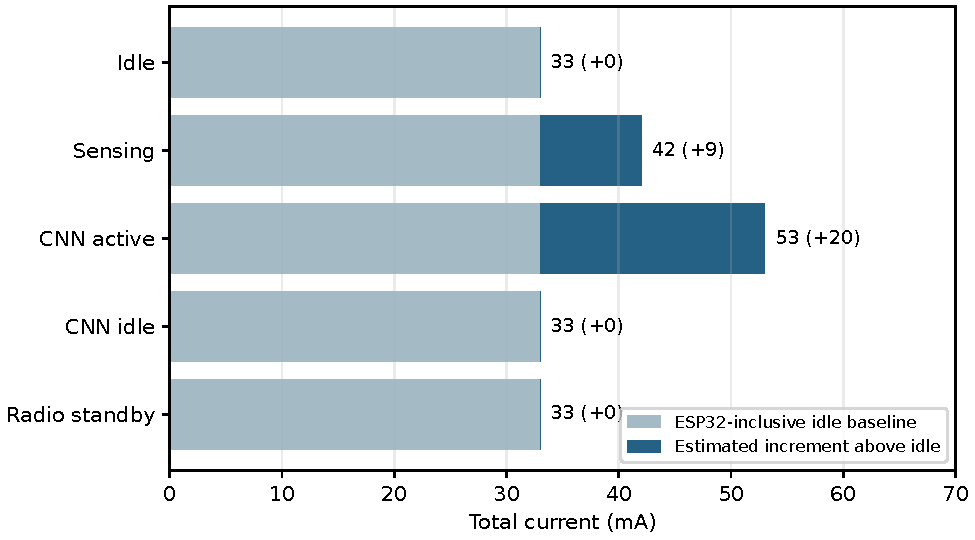
\includegraphics[width=0.9\textwidth]{figures/operating_mode_current.pdf}
\caption{\newrevision{ESP32-inclusive readings split into the 33 mA idle baseline and estimated increments. Equal indicated readings do not establish zero component consumption.}}
\label{fig:mode_current}
\end{figure}

\begin{table}[htbp]
\centering
\caption{\newrevision{LoRa transmission current at 3.3 V and calculated power and energy. Energy calculations use the full indicated current.}}
\label{tab:lora_power}
\begin{tabular}{rrrrrr}
\toprule
TX setting & Current & Power & Run energy & Packet energy & DATA energy \\
(dBm) & (mA) & (mW) & (J) & (mJ) & (mJ/byte) \\
\midrule
10 & 20 & 66 & 2.8 & 2.8 & 0.35 \\
15 & 30 & 99 & 4.2 & 4.2 & 0.52 \\
17 & 40 & 132 & 5.5 & 5.5 & 0.69 \\
19 & 60 & 198 & 8.3 & 8.3 & 1.04 \\
\bottomrule
\end{tabular}
\end{table}

\newrevision{Measurement repeatability and instrument accuracy remain unquantified. The table reports rounded energy values.}

\newrevision{Power is calculated as $P=VI$, run energy as $E=Pt$, and energy per packet as $E/N$, using a 42 s run and 1,000 transmitted packets per setting. Energy per DATA byte divides packet energy by eight, the DATA packet length in this experiment. The calculations assume the indicated current represents the run average. The measurement instrument, repetition count, radio parameters, receiver delivery count, and measurement boundary remain undocumented. The results estimate run energy and energy per transmitted packet and DATA byte.}

\begin{figure}[htbp]
\centering
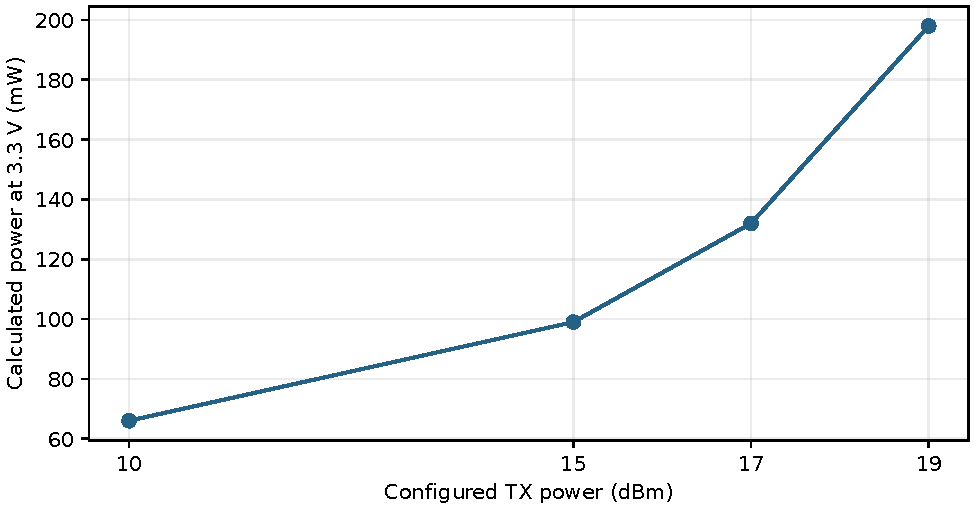
\includegraphics[width=0.9\textwidth]{figures/lora_power_sweep.pdf}
\caption{\newrevision{Calculated LoRa power at a 3.3 V supply for four transmit-power settings.}}
\label{fig:lora_power_sweep}
\end{figure}

\newrevision{Calculated power rises from 66 mW at 10 dBm to 198 mW at 19 dBm, a threefold increase. Selecting a TX setting also requires packet-delivery and range measurements under the permitted local radio settings. The 3.3 V sweep and the operating-mode measurements characterize separate test setups. Comparing their readings requires equivalent supply conditions and measurement boundaries.}
\FloatBarrier

\label{sec:PerformanceAnalysisPlan}

The performance analysis will compare the behavior of the system across the sensing, communication, and classification stages. The planned analysis will examine whether the acoustic sensor can capture usable signals, whether the wireless network can deliver those signals reliably, and whether the classifier can produce useful detection results in noisy conditions. The final system will also be assessed for responsiveness and monitoring usefulness through the dashboard.

For Senior Design I, the main goal of this section is to define a clear evaluation framework that can be executed in Senior Design II. The project will therefore use this plan to guide implementation, testing, and future experimental analysis.

\newrevision{The communication analysis will retain the baseline packet, compact packet, and any split-learning packet as separate variants. It will report payload bytes, airtime, packet loss, and energy for each variant, plus ESP32 memory/runtime for the split-learning variant. A smaller packet is useful only when it preserves the required detection performance.}

\chapter{Project Management}
\label{ch:ProjectManagement}

% ===============================
% CHAPTER 7: PROJECT MANAGEMENT
% ===============================

\section{Software Lifecycle}
\label{sec:SWLifecycle}

\subsection{Overview and Rationale}

\earlierrevision{The project combines hardware, embedded firmware, wireless networking, cloud software, and machine learning. Each subsystem depends on experimental results, especially sensor coupling, outdoor noise, communication reliability, and model performance. The team therefore uses an Agile-Spiral hybrid: each spiral addresses a major technical risk, while short iterations produce and test a working increment.}

\subsection{Justification for the Agile-Spiral Model}

\earlierrevision{A strictly sequential process would force the team to finalize choices before field evidence is available. Sensor placement, trunk properties, wind, rain, and background activity can all affect signal quality. Model selection also requires repeated training and evaluation on leakage-safe data splits. At the same time, hardware coupling, radio reliability, and power consumption need explicit risk reviews before later work depends on them. The hybrid model fits these needs by combining iterative development with a risk checkpoint at the end of each spiral.}

\subsection{Model Structure and Phases}

The Agile-Spiral life cycle adopted for this project consists of five major spiral iterations, each structured around four quadrants consistent with Boehm's original Spiral Model formulation: (1) Determine objectives, (2) Identify and resolve risks, (3) Develop and test, and (4) Plan the next iteration. Within the development and test quadrant of each spiral, Agile sprint cycles of two to three weeks are conducted to produce testable increments of the system.

\earlierrevision{The five spiral iterations cover the six design objectives in Section 1.4. Objectives 4 and 5 are combined in the integration and field-validation spiral, while Objective 6 is delivered through the deployment guides and calibration procedures produced at the end of that spiral.}

\begin{table}[h!]
\centering
\caption{Agile-Spiral Iteration Plan}
\label{tab:spiral_plan}
\renewcommand{\arraystretch}{1.3}
\begin{tabular}{>{\raggedright\arraybackslash}p{2.2cm} >{\raggedright\arraybackslash}p{3.8cm} >{\raggedright\arraybackslash}p{3.8cm} >{\raggedright\arraybackslash}p{1.8cm}}
\toprule
\textbf{Spiral / Phase} & \textbf{Primary Objectives} & \textbf{Key Deliverables} & \textbf{Duration} \\
\midrule
Spiral 1: Requirements \& Architecture &
Finalize system architecture; define sensor node hardware specifications; establish dataset and labeling strategy &
System architecture diagram; hardware BoM; dataset acquisition plan &
3 weeks \\
Spiral 2: Acoustic Sensing Unit &
Prototype piezoelectric sensing node; calibrate the mechanical exciter and reference sensor; run controlled wood-plank trials; implement bandpass filtering pipeline &
\newrevision{Functional sensor node prototype; calibrated bench apparatus; controlled wood-plank test report} &
4 weeks \\
Spiral 3: Wireless Sensor Network &
Implement WSN architecture; compare baseline and compact LoRa packets; optimize power management; environmental enclosure &
\newrevision{Communication reliability report; packet-compaction comparison; power consumption analysis} &
4 weeks \\
Spiral 4: Deep Learning Classifier &
Train and validate CNN/BiLSTM/hybrid classifiers on TreeVibes dataset; compare one feasible split-learning point; optimize hyperparameters; 10-fold cross-validation &
\newrevision{Selected classification model; split-learning feasibility comparison; confusion matrix; recall, false-negative rate, F1 score, and cross-validation variance report} &
5 weeks \\
Spiral 5: Integration \& Field Validation &
Cloud platform integration; dashboard development; end-to-end testing; live-palm validation only where naturally infested palms are available &
\newrevision{Monitoring dashboard; bench-validation report; live-palm validation report only if available; final performance metrics} &
4 weeks \\
\bottomrule
\end{tabular}
\end{table}

\newrevision{The phase gate after the wood-plank campaign requires the team to review playback fidelity, SNR versus distance, and recall versus distance/noise before making a live-palm claim. If naturally infested palms are unavailable, the team will complete the emulation study and report it as controlled bench validation rather than as proof of real RPW detection.}

\FloatBarrier

\subsection{Agile Practices Within Each Spiral Iteration}

Within each spiral iteration, the development team applies core Agile engineering practices to manage task decomposition, progress tracking, and quality assurance. These include:

\begin{itemize}
    \item \textbf{Sprint Planning:} At the start of each two-to-three-week sprint, team members
    identify and assign user stories and engineering tasks relevant to the active spiral
    objective. Tasks are drawn from a maintained product backlog and prioritized based on
    risk criticality and functional dependencies.

    \item \textbf{Iterative Prototyping and Testing:} Hardware and software components are built in
    small, testable increments. Each sprint concludes with a working prototype or testable
    software module. This enables rapid detection of integration failures. For instance,
    incompatibility between the microcontroller sampling rate and the cloud preprocessing
    pipeline before they propagate to later development stages.

    \item \earlierrevision{\textbf{Continuous Integration and Validation:} Automated training and evaluation scripts
    are run after changes to the model or data pipeline. Recall is the primary selection metric,
    with false-negative rate, precision, F1 score, and data-split variance reported alongside it.}

    \item \textbf{Sprint Review and Retrospective:} Each sprint concludes with a structured review in
    which completed increments are demonstrated to advisors (Dr. Mohamed Alhajri and Dr.
    Taha Landolsi) for validation against the project objectives. A retrospective session
    identifies process impediments and adjusts task allocation for the subsequent sprint.

    \item \textbf{Risk Register Maintenance:} Consistent with the Spiral Model's risk-driven
    approach, a living risk register is maintained throughout the project. Risks identified
    during each spiral, including environmental noise interference, sensor calibration drift,
    and wireless packet loss under field conditions are formally assessed, prioritized, and
    mitigated before progressing to the next iteration.
\end{itemize}

\subsection{Comparison with Alternative Life Cycle Models}

The Waterfall model was considered but rejected due to its requirement for fully specified, stable requirements prior to development commencement. As the literature review established (Section 2.6), the performance of acoustic classification systems in real-world outdoor environments is heavily dataset- and environment-specific, making it impossible to define precise performance targets and implementation approaches without empirical feedback from prototype testing.

A purely Agile approach such as Scrum was considered as an alternative. While Scrum's sprint-based delivery mechanism is well-suited to the software components of this project, it lacks the explicit risk management framework necessary for managing the hardware uncertainty inherent in deploying piezoelectric sensors in outdoor plantation environments. The Spiral Model's formal risk assessment quadrant addresses this gap directly.

The V-Model was also evaluated but found unsuitable, as it assumes a sequential design process with verification stages tightly coupled to corresponding development stages. The feedback-driven nature of machine learning model development where training, evaluation, and architectural modification cycles are interleaved does not align with the V-Model's linear structure.

\earlierrevision{The Agile-Spiral hybrid was selected because it supports repeated model and hardware evaluation while keeping major technical risks visible within the fixed academic schedule.}

\subsection{Traceability to Design Objectives}

Each spiral iteration maintains full traceability to the project's design objectives as defined in Section 1.4. The mapping ensures that every development activity is anchored to a measurable, verifiable deliverable:

\begin{itemize}
    \item Spiral 1 supports Objectives 1.4.1 and 1.4.6 by establishing the hardware
    specifications and deployment architecture that govern all subsequent spirals.

    \item Spiral 2 directly addresses Objective 1.4.1 the development and laboratory
    validation of a low-cost acoustic sensing unit capable of detecting larval vibrations within
    a 1.5 to 2.0 meter radius.

    \item Spiral 3 addresses Objective 1.4.2 the implementation of a scalable Wireless Sensor
    Network architecture with validated communication reliability, power management, and
    environmental robustness.

    \item \earlierrevision{Spiral 4 addresses Objective 1.4.3: design, train, and validate the acoustic classifier,
    prioritize recall, report supporting metrics, and assess variation through 10-fold
    cross-validation.}

    \item Spiral 5 addresses Objectives 1.4.4 and 1.4.5 the integration of the cloud-based
    monitoring platform and the execution of end-to-end field validation against conventional
    inspection practices.
\end{itemize}

This traceability structure ensures that the life cycle model functions not merely as a development process, but as a quality assurance framework that ties every sprint deliverable back to the project's stated technical and operational requirements.

\section{Work Breakdown Structure}
\label{sec:WBS}

\subsection{Top Level Work}

\earlierrevision{The Work Breakdown Structure (WBS) divides the project into five packages: (1) Requirements \& Architecture, (2) Acoustic Sensing Unit, (3) Wireless Sensor Network, (4) Deep Learning Classifier, and (5) Integration \& Field Validation. Together, these packages cover the design, implementation, and validation of the complete prototype. The following subsections summarize the purpose and outputs of each package.}

\begin{figure}[H]
\centering
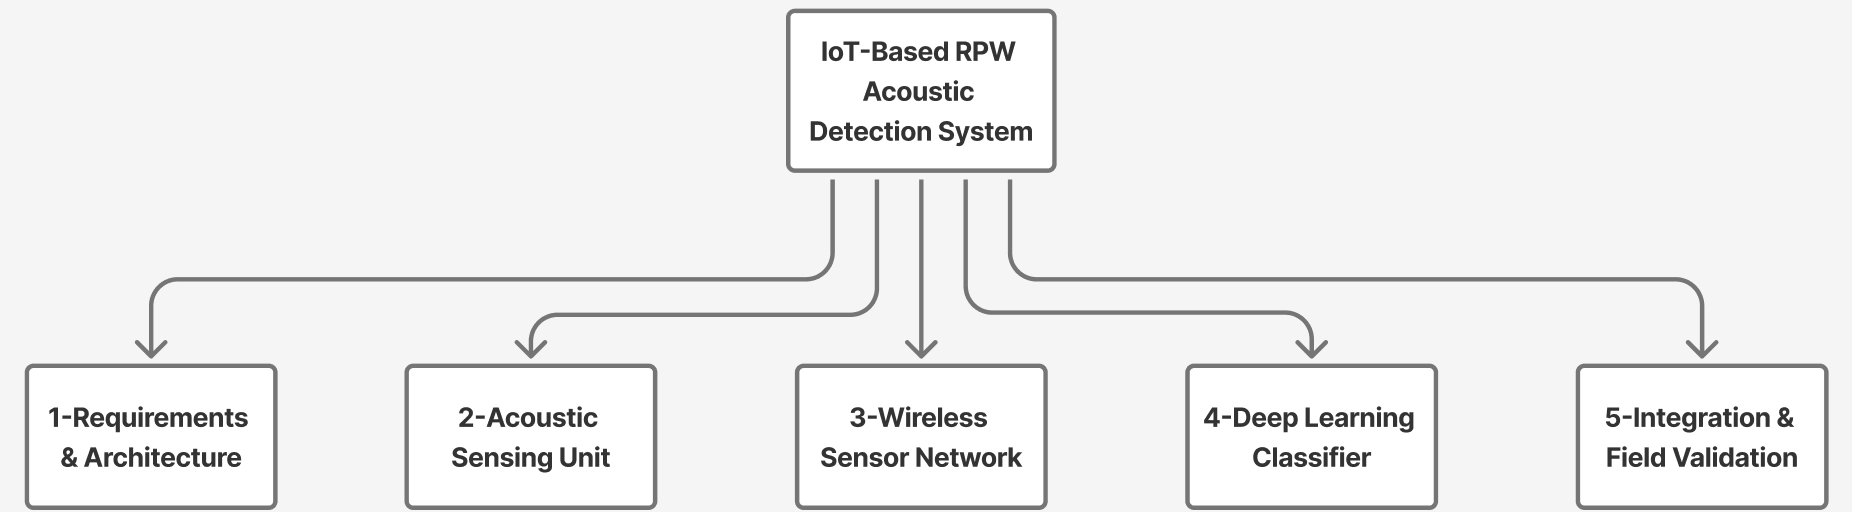
\includegraphics[width=0.85\textwidth]{figures/TLP.png}
\caption{Top Level Breakdown}
\label{fig:wbs_toplevel}
\end{figure}

\subsection{WP1 --- Requirements \& Architecture}

This work package establishes the technical and operational foundation for the entire system. It encompasses four tasks: defining the overall system architecture and interface specifications; preparing the hardware bill of materials; planning the acoustic dataset acquisition process; and designing the labeling strategy that will guide supervised model training. Outputs from this package directly inform all subsequent work packages.

\begin{figure}[H]
\centering
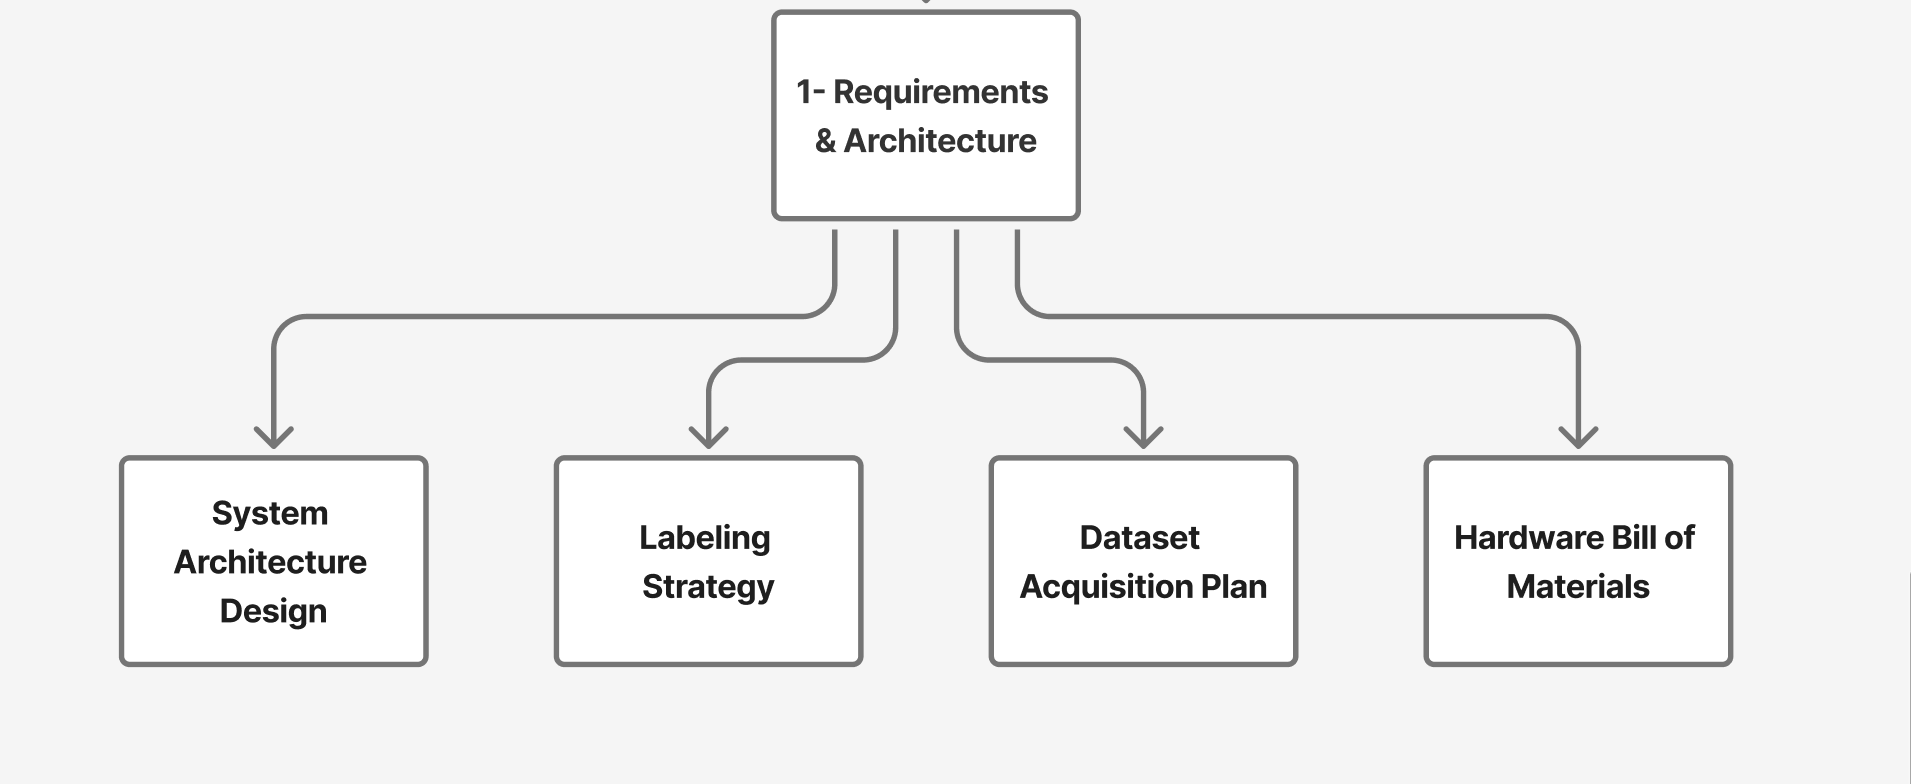
\includegraphics[width=0.85\textwidth]{figures/WP1.png}
\caption{WP1 --- Requirements \& Architecture}
\label{fig:wbs_wp1}
\end{figure}

\subsection{WP2 --- Acoustic Sensing Unit}

The Acoustic Sensing Unit translates RPW mechanical vibrations inside palm tree trunks into clean electrical signals ready for wireless transmission. The five tasks span hardware prototyping of piezoelectric sensors, integration of metallic waveguides to amplify acoustic coupling, construction of the signal acquisition pipeline, implementation of bandpass filters to isolate the RPW frequency band, and a controlled lab validation campaign to confirm performance before field deployment.

\begin{figure}[H]
\centering
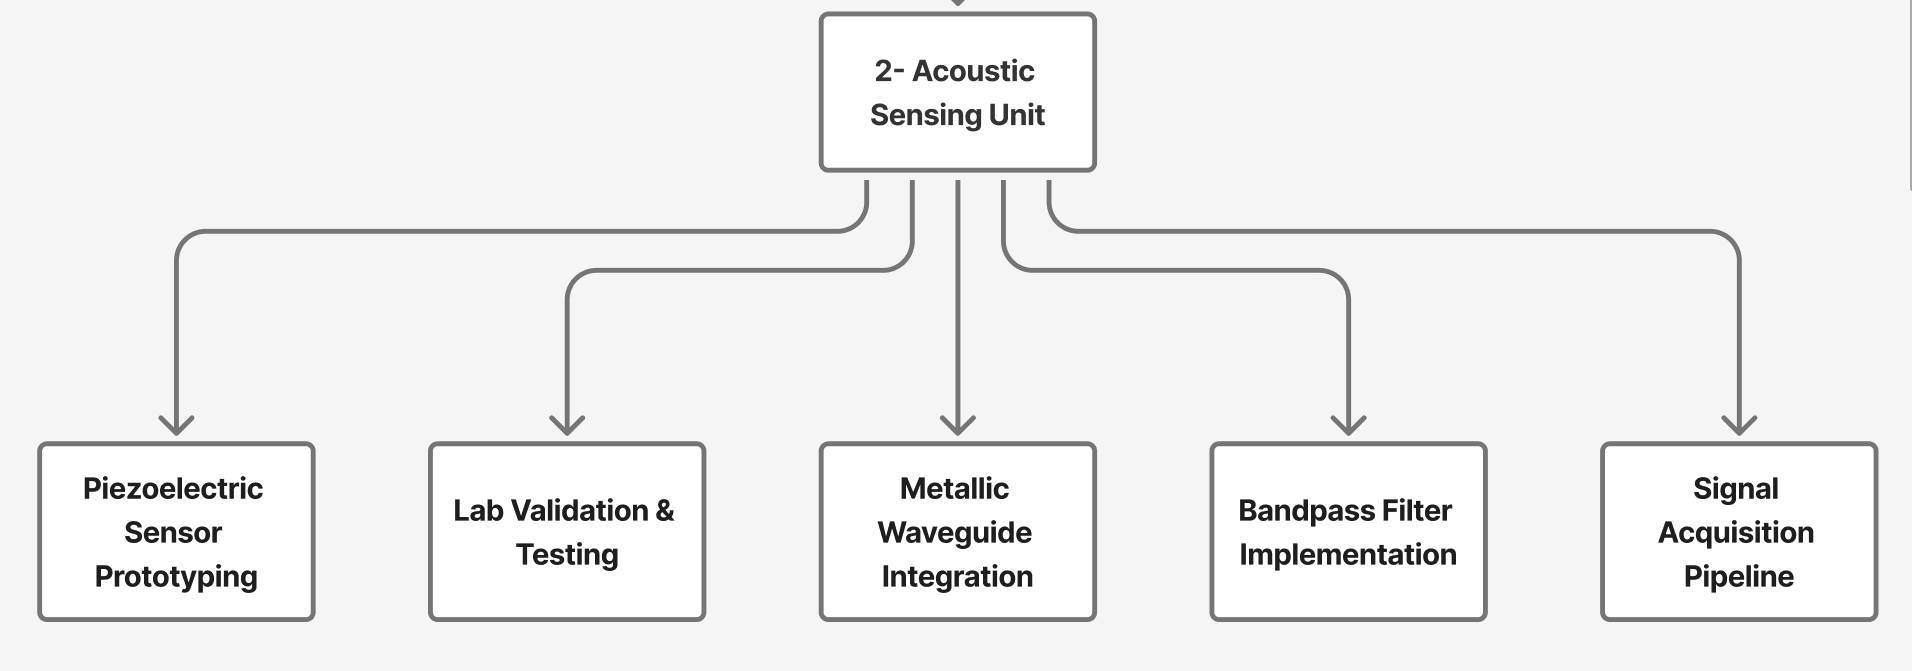
\includegraphics[width=0.85\textwidth]{figures/WP2.png}
\caption{WP2 --- Acoustic Sensing Unit}
\label{fig:wbs_wp2}
\end{figure}

\subsection{WP3 --- Wireless Sensor Network}

The Wireless Sensor Network (WSN) package ensures that acoustic data collected by individual sensing nodes is reliably transmitted to the cloud processing backend. Tasks address WSN topology design, selection and configuration of LoRa communication modules, power management strategies for extended battery life in remote plantations, weatherproof enclosure design, and the multi-node deployment and integration tests that confirm network-wide reliability.

\begin{figure}[H]
\centering
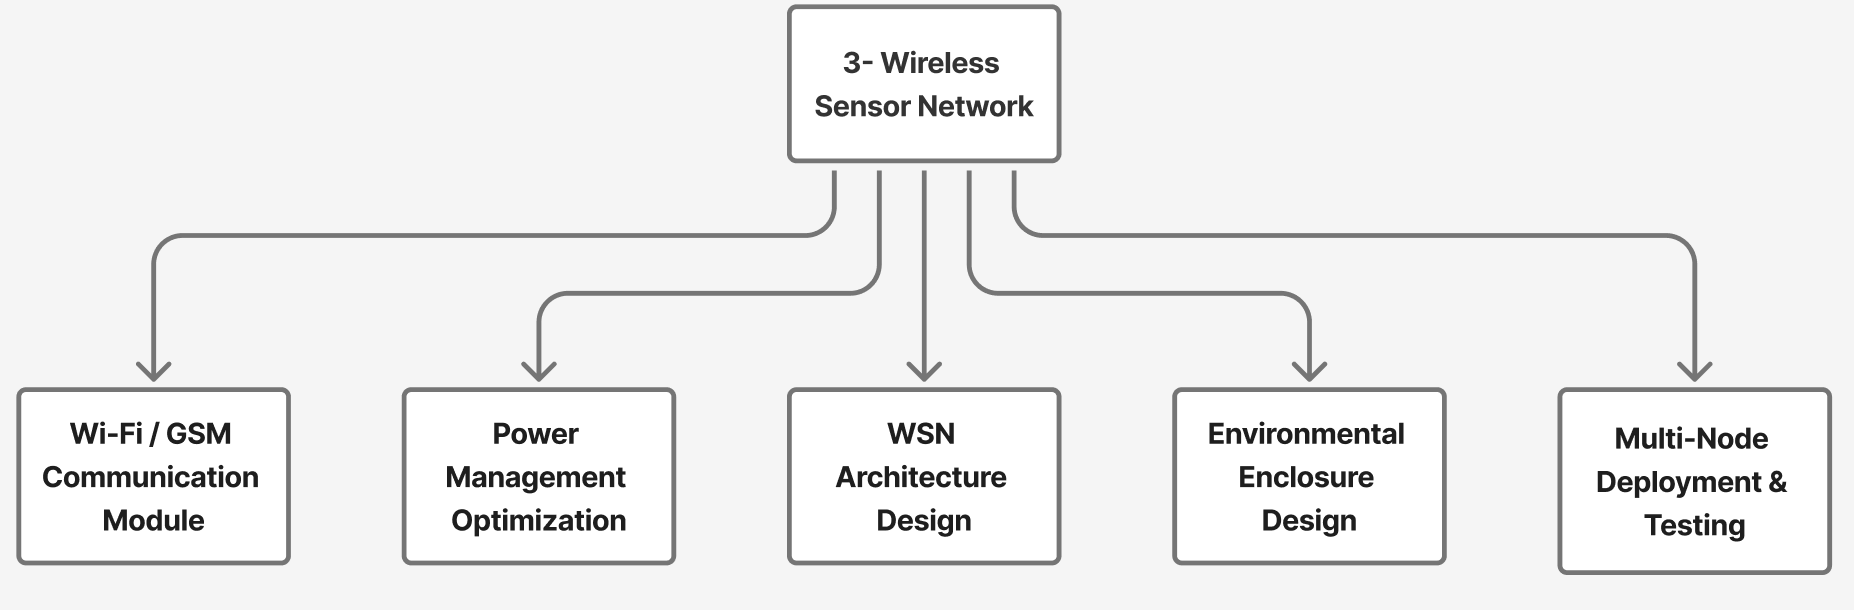
\includegraphics[width=0.85\textwidth]{figures/WP3.png}
\caption{WP3 --- Wireless Sensor Network}
\label{fig:wbs_wp3}
\end{figure}

\subsection{WP4 --- Deep Learning Classifier}

The Deep Learning Classifier is the intelligence core of the system. It processes raw acoustic data through a multi-stage pipeline: data preprocessing and augmentation to improve model generalization; feature extraction using four complementary spectral representations; and training of three candidate model architectures --- CNN Transfer Learning, BiLSTM, and a CNN-LSTM Hybrid. Hyperparameter tuning and 10-fold cross-validation ensure rigorous, reproducible performance estimation. Task 4.2 (Feature Extraction) is further broken down into four sub-tasks covering MFCC, BFCC, CQCC, and STFT Spectrogram methods.

\begin{figure}[H]
\centering
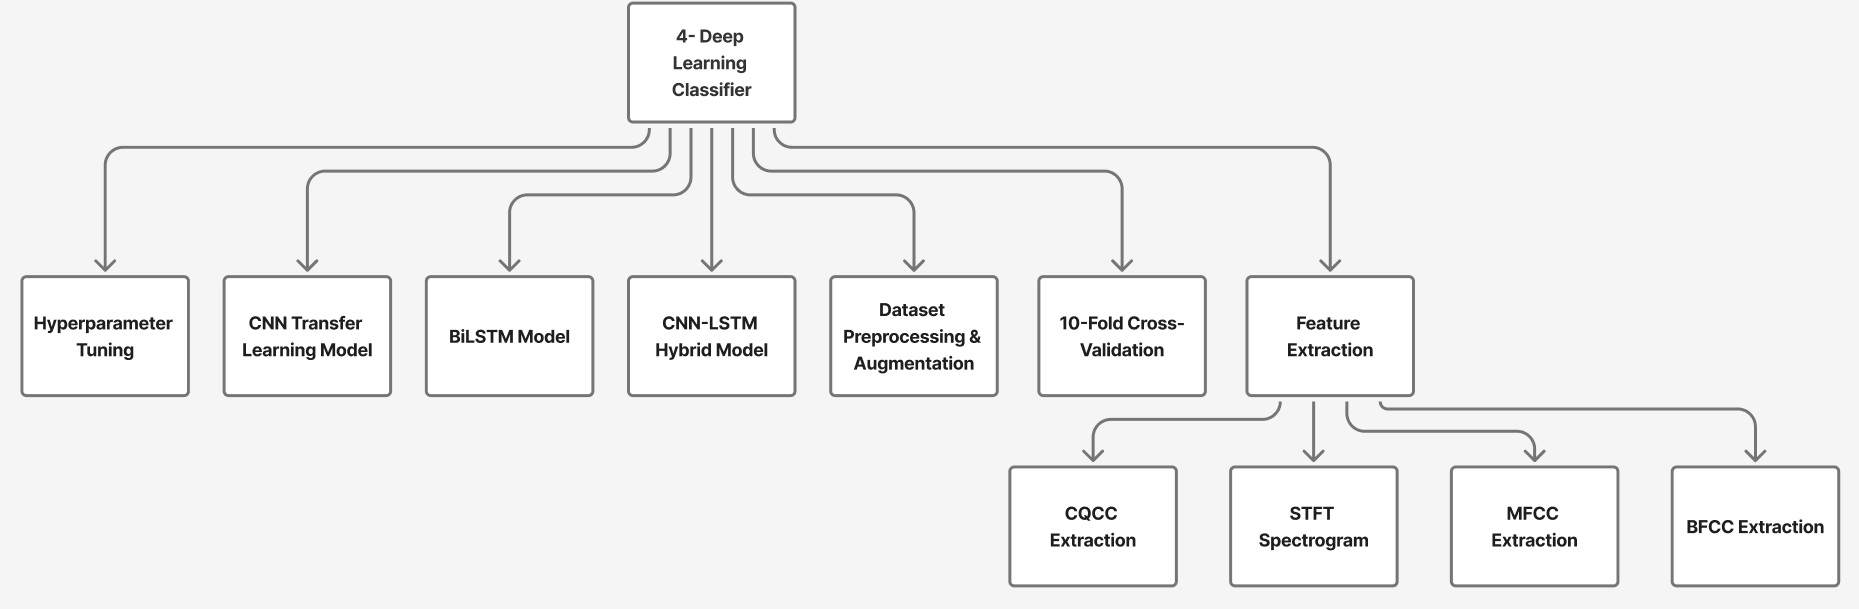
\includegraphics[width=0.85\textwidth]{figures/WP4.png}
\caption{WP4 --- Deep Learning Classifier}
\label{fig:wbs_wp4}
\end{figure}

\subsection{WP5 --- Integration \& Field Validation}

The final work package closes the loop by deploying the full system end-to-end in real agricultural environments. Seven tasks cover cloud infrastructure provisioning, automated preprocessing pipelines, the model inference and alert engine, a real-time monitoring dashboard for farm operators, field deployment and sensor calibration at palm plantation sites, holistic end-to-end system validation, and a head-to-head comparative analysis against conventional manual inspection methods to quantify the detection advantages offered by the IoT solution.

\begin{figure}[H]
\centering
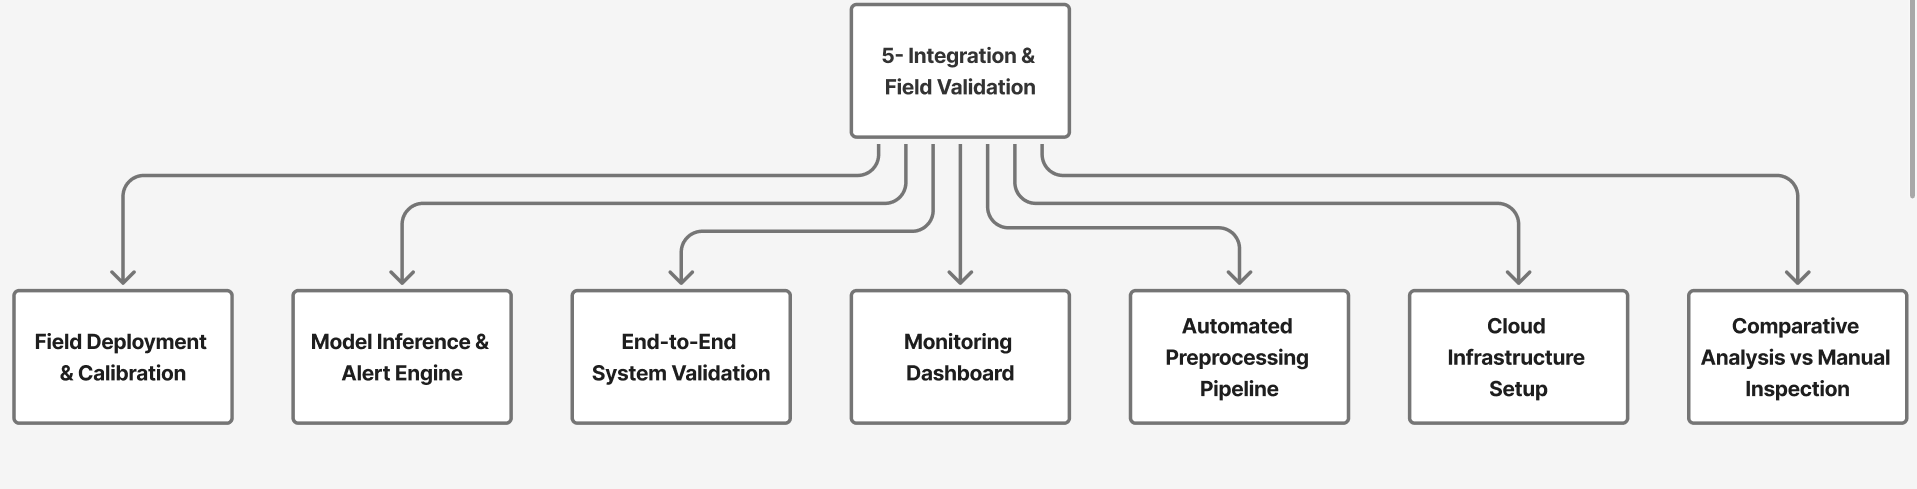
\includegraphics[width=0.85\textwidth]{figures/WP5.png}
\caption{WP5 --- Integration \& Field Validation}
\label{fig:wbs_wp5}
\end{figure}

\section{Project Schedule and Resource Assignments (Gantt Chart)}
\label{sec:Schedule}

\earlierrevision{The schedule covers six objectives from January to June 2026. Some tasks overlap so that hardware, networking, and machine-learning work can progress in parallel, while integration tasks depend on earlier prototype outputs. Table~\ref{tab:gantt} assigns a lead, support member where needed, and a delivery window to each task. Progress is reviewed weekly, and delays that affect integration are recorded in the risk register and reflected in the next iteration plan.}

\renewcommand{\arraystretch}{1.3}
\begin{longtable}{>{\raggedright\arraybackslash}p{6.5cm} >{\raggedright\arraybackslash}p{2.8cm} >{\raggedright\arraybackslash}p{1.8cm} >{\raggedleft\arraybackslash}p{1.8cm}}
\caption{RPW Detection System --- Project Schedule with Resource Assignments (January -- June 2026)}\label{tab:gantt}\\
\toprule
\textbf{Task / Deliverable} & \textbf{Schedule} & \textbf{Lead} & \textbf{Support} \\
\midrule
\multicolumn{4}{l}{\textbf{O1 $\cdot$ Acoustic Sensing Unit (Spiral 1--2)}} \\
Physical Sensor Assembly \& Waveguide & Jan 19 -- Feb 2 & Abdurrahman & --- \\
MCU Programming \& ADC Sampling & Jan 19 -- Feb 2 & Khalid & --- \\
Analog Signal Conditioning \& Pre-filtering & Jan 26 -- Feb 5 & Khalid & --- \\
Bandpass Filter Pipeline 100--2500 Hz & Feb 2 -- Feb 9 & Khalid & --- \\
Outdoor Enclosure \& Rugged Casing & Feb 2 -- Feb 9 & Abdurrahman & --- \\
Lab Signal Validation & Feb 9 -- Feb 16 & Abdurrahman & Khalid \\
\midrule
\multicolumn{4}{l}{\textbf{O2 $\cdot$ Wireless Sensor Network (Spiral 3)}} \\
WSN Topology \& Protocol Design & Feb 16 -- Feb 23 & Kareem & --- \\
LoRa Module Config \& Packet Formatting & Feb 23 -- Mar 5 & Kareem & --- \\
MCU $\leftrightarrow$ Wireless Firmware \& Scheduling & Feb 23 -- Mar 5 & Khalid & Kareem \\
Solar Panel \& Power Regulation Circuit & Feb 23 -- Mar 2 & Abdurrahman & --- \\
Network Reliability \& Sync Testing & Mar 9 -- Mar 16 & Kareem & Abdurrahman, Khalid \\
\midrule
\multicolumn{4}{l}{\textbf{O3 $\cdot$ Deep Learning Classifier (Spiral 4)}} \\
Dataset Preprocessing \& Augmentation & Mar 16 -- Mar 23 & Khalid & --- \\
Feature Extraction --- MFCC / BFCC / CQCC / STFT & Mar 16 -- Mar 26 & Khalid & --- \\
CNN Transfer Learning Model & Mar 23 -- Apr 2 & Haitham & --- \\
BiLSTM Model Architecture & Mar 23 -- Apr 2 & Haitham & --- \\
CNN-LSTM Hybrid Model & Apr 6 -- Apr 13 & Haitham & Khalid \\
Hyperparameter Tuning & Apr 13 -- Apr 20 & Haitham & Khalid \\
10-Fold Cross-Validation (variance $<$ 3\%) & Apr 13 -- Apr 20 & Haitham & Khalid \\
\midrule
\multicolumn{4}{l}{\textbf{O4 $\cdot$ Cloud Platform \& Dashboard (Spiral 5)}} \\
Cloud Server Setup \& Data Ingestion API & Apr 20 -- Apr 27 & Kareem & --- \\
Database Schema \& Security Setup & Apr 20 -- Apr 25 & Kareem & --- \\
Model Inference Service Deployment & Apr 27 -- May 4 & Haitham & --- \\
Automated Preprocessing on Server & Apr 27 -- May 4 & Haitham & --- \\
Alert Threshold Logic \& Delivery & May 4 -- May 9 & Kareem & Haitham \\
Monitoring Dashboard UI & May 4 -- May 11 & Kareem & --- \\
\midrule
\multicolumn{4}{l}{\textbf{O5 $\cdot$ Field Testing \& Validation}} \\
Hardware Durability \& Weatherproofing Checks & May 11 -- May 18 & Abdurrahman & --- \\
Network Stability \& Latency Logging & May 11 -- May 18 & Kareem & --- \\
Signal Quality \& Noise Benchmarking & May 11 -- May 18 & Khalid & --- \\
Model Accuracy vs Manual Inspection & May 11 -- May 18 & Haitham & --- \\
End-to-End System Validation & May 18 -- May 25 & All & --- \\
\midrule
\multicolumn{4}{l}{\textbf{O6 $\cdot$ Field Deployment \& Calibration}} \\
Physical Installation \& Mounting Guide & May 25 -- May 30 & Abdurrahman & --- \\
Network Configuration \& Expansion Guide & May 25 -- May 30 & Kareem & --- \\
Sensor Calibration \& Signal Verification Procedure & May 25 -- May 30 & Khalid & --- \\
Model Retraining \& Update Procedure & May 25 -- May 30 & Haitham & --- \\
End-to-End Integration Guide & May 28 -- Jun 2 & Khalid & Kareem \\
\bottomrule
\multicolumn{4}{l}{\footnotesize Note: ``Lead'' denotes the primary responsible team member; ``Support'' indicates a secondary} \\
\multicolumn{4}{l}{\footnotesize contributor. A dash (---) indicates no supporting member was assigned for that task.} \\
\end{longtable}

\clearpage
\begin{landscape}
\thispagestyle{plain}
\begin{figure}[p]
\centering
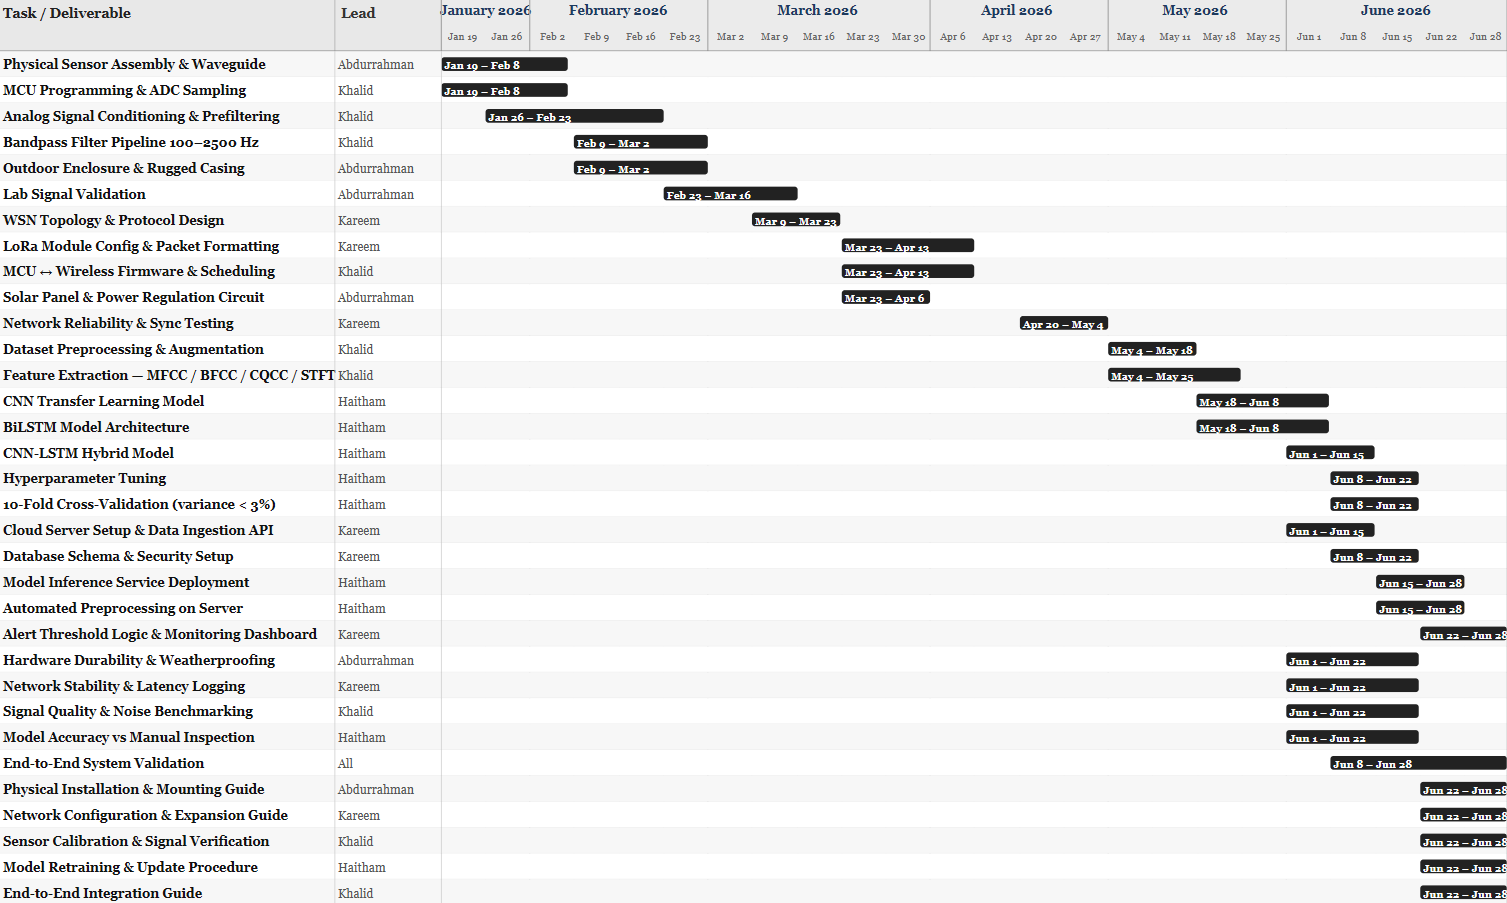
\includegraphics[width=\linewidth,height=1.12\textheight,keepaspectratio]{figures/The Gantt Chart.png}
\caption{Project Gantt Chart}
\label{fig:gantt_chart}
\end{figure}
\end{landscape}
\clearpage
\section{Team Organization}
\label{sec:TeamOrg}

\earlierrevision{The team includes three Computer Engineering students---Khalid Hamdan, Kareem Mahmoud, and Abdurrahman Maricar---and one Computer Science student, Haitham Ayyash. Their combined experience covers embedded systems, wireless networking, cloud software, and deep learning.}

\earlierrevision{The team uses a flat decision-making structure. Each member leads assigned technical work and presents progress, evidence, and blockers at the weekly meeting. Decisions are made by team consensus and reviewed with the project advisors, Dr. Mohamed Alhajri and Dr. Taha Landolsi, when they affect scope, safety, or major design choices.}

\earlierrevision{The role tables use three labels. A \emph{Lead} coordinates an objective and is accountable for its acceptance criteria. \emph{Support} contributes to work led by another member. An \emph{Owner} is accountable for a clearly bounded task within a shared objective. During field testing and deployment, all members are owners of different tasks in their own areas; this does not mean that every member owns the entire objective.}

\begin{table}[H]
\centering
\caption{Khalid Hamdan --- Roles and Responsibilities}
\label{tab:roles_khalid}
\renewcommand{\arraystretch}{1.3}
\begin{tabular}{>{\raggedright\arraybackslash}p{3.5cm} p{1.8cm} p{8.0cm}}
\toprule
\textbf{Objective} & \textbf{Role} & \textbf{Tasks} \\
\midrule
Acoustic Sensing Unit & Support & Microcontroller programming; ADC sampling rate
configuration; analog signal conditioning circuitry; on-device
pre-filtering pipeline \\
Wireless Sensor Network & Support & MCU wireless module firmware; buffering and transmission
scheduling logic \\
Deep Learning Classifier & Lead & Signal preprocessing pipeline; feature extraction (MFCC,
BFCC, CQCC, STFT spectrograms); dataset preparation and
augmentation; TinyML edge inference feasibility study \\
Field Testing \& Validation & Owner & Signal quality validation in-field; noise condition
benchmarking (wind, birds, machinery) \\
Deployment \& Documentation & Owner & Sensor calibration and signal verification procedure; joint
authorship of system integration guide \\
\bottomrule
\end{tabular}
\end{table}

\begin{table}[H]
\centering
\caption{Kareem Mahmoud --- Roles and Responsibilities}
\label{tab:roles_kareem}
\renewcommand{\arraystretch}{1.3}
\begin{tabular}{>{\raggedright\arraybackslash}p{3.5cm} p{1.8cm} >{\raggedright\arraybackslash}p{8.0cm}}
\toprule
\textbf{Objective} & \textbf{Role} & \textbf{Tasks} \\
\midrule
Wireless Sensor Network & Lead & WSN topology and protocol design; LoRa module
configuration; data packet formatting and transmission;
network reliability and synchronization testing \\
Cloud Platform \& Dashboard & Lead & Cloud server setup and data ingestion API; database schema
for acoustic readings and alerts; network security and access
control; alert delivery (SMS/email/push) \\
Field Testing \& Validation & Owner & Network stability and uptime measurement; data loss rate and
latency logging \\
Deployment \& Documentation & Owner & Network configuration and expansion guide; joint authorship
of system integration guide \\
\bottomrule
\end{tabular}
\end{table}

\begin{table}[H]
\centering
\caption{Abdurrahman Maricar --- Roles and Responsibilities}
\label{tab:roles_abd}
\renewcommand{\arraystretch}{1.3}
\begin{tabular}{>{\raggedright\arraybackslash}p{3.5cm} p{1.8cm} >{\raggedright\arraybackslash}p{8.0cm}}
\toprule
\textbf{Objective} & \textbf{Role} & \textbf{Tasks} \\
\midrule
O1: Acoustic Sensing Unit & Lead & Physical sensor assembly and mounting; piezoelectric
element selection and coupling; metallic waveguide design
and installation; outdoor enclosure and rugged casing \\
O2: Wireless Sensor Network & Support & Physical integration of wireless modules onto node PCB;
solar panel and battery power circuit; power regulation
components \\
O5: Field Testing \& Validation & Owner & Hardware durability and weatherproofing checks; physical
sensor re-mounting and re-calibration \\
O6: Field Deployment \& Calibration & Owner & Physical installation and mounting guide \\
\bottomrule
\end{tabular}
\end{table}

\begin{table}[H]
\centering
\caption{Haitham Ayyash --- Roles and Responsibilities}
\label{tab:roles_haitham}
\renewcommand{\arraystretch}{1.3}
\begin{tabular}{>{\raggedright\arraybackslash}p{3.5cm} p{1.8cm} >{\raggedright\arraybackslash}p{8.0cm}}
\toprule
\textbf{Objective} & \textbf{Role} & \textbf{Tasks} \\
\midrule
O3: Deep Learning Classifier & Lead & CNN/BiLSTM/hybrid model architecture design; model
training, fine-tuning, and hyperparameter search; 10-fold
cross-validation and variance analysis ($<$3\%); confusion
matrix, precision, and recall evaluation \\
O4: Cloud Platform \& Dashboard & Support & Model inference service deployment; automated
preprocessing on server side; alert threshold logic and
confidence scoring \\
O5: Field Testing \& Validation & Owner & Model accuracy comparison against conventional inspection;
false positive and negative analysis on field data \\
O6: Field Deployment \& Calibration & Owner & Model retraining and update procedure \\
\bottomrule
\end{tabular}
\end{table}

\clearpage

\section{\earlierrevision{Cost Analysis}}
\label{sec:Budget}

\earlierrevision{Table~\ref{tab:bom} estimates the purchase cost of one breadboard sensing-node prototype and one cluster-head prototype in AED. The estimate is suitable for prototype planning, not for a complete farm deployment. It excludes delivery, taxes, enclosure fabrication, PCB production, sensor mounting hardware, optional solar charging, cellular service, cloud hosting, installation labor, maintenance, and replacement parts. Software licenses are estimated at zero because the planned tools use open-source or community editions; this does not imply zero operating cost.}

\begin{table}[H]
    \centering
    \caption{\earlierrevision{Prototype bill of materials and cost estimate (AED).}}
    \label{tab:bom}
    \renewcommand{\arraystretch}{1.3}
    \resizebox{\textwidth}{!}{%
    \begin{tabular}{cl>{\raggedright\arraybackslash}p{5.2cm}ccc}
        \toprule
        \textbf{No.} & \textbf{Component} & \textbf{Description} & \textbf{Qty} & \textbf{Unit (AED)} & \textbf{Subtotal (AED)} \\
        \midrule
        \multicolumn{6}{l}{\earlierrevision{\textit{Sensing-node prototype}}} \\
		1  & Microcontroller     & ESP32 dev board (Wi-Fi/Bluetooth, dual-core)       & 1 & 25.00 & 25.00 \\
		2  & Piezo sensor        & 27~mm piezoelectric disc                            & 1 & 2.00  & 2.00  \\
		3  & Op-amp IC           & MCP6002 SOP-8                                      & 1 & 1.20  & 1.20  \\
		4  & LoRa module         & HopeRF RFM95W (915 MHz)                     		& 1 & 24.95 & 24.95 \\
		5  & LoRa antenna        & 915~MHz omni antenna (RP-SMA)                      & 1 & 48.67 & 48.67 \\
		6  & Breadboard          & 400-tie breadboard                                 & 1 & 5.00  & 5.00  \\
		7  & Wiring              & Jumper wire pack                                   & 1 & 20.00 & 20.00 \\
		8  & USB cable           & Micro-USB cable                                    & 1 & 10.00 & 10.00 \\
		9 & Battery             & 18650 Li-ion battery (3.7~V)                       & 1 & 2.50  & 2.50  \\
		10 & Voltage regulator   & AMS1117 3.3~V LDO (SOT-223)                        & 1 & 4.00  & 4.00  \\
        \midrule
        \multicolumn{6}{l}{\earlierrevision{\textit{Cluster-head prototype}}} \\
		11 & Microcontroller     & Raspberry Pi 4 starter kit (4~GB + 64~GB microSD) & 1 & 560.00 & 560.00 \\
		12 & LoRa module         & HopeRF RFM95W (915 MHz)                    		 & 1 & 24.95  & 24.95  \\
		13 & LoRa antenna        & 915~MHz omni antenna (RP-SMA)                      & 1 & 48.67  & 48.67  \\
		14 & Wiring              & Jumper wire pack                                   & 1 & 7.00   & 7.00   \\
		15 & Power supply        & 5~V/3~A USB-C wall adapter                         & 1 & 40.00  & 40.00  \\
        \midrule
        \multicolumn{4}{l}{\textit{Software}} & \multicolumn{2}{r}{\textit{All tools free}} \\
        \midrule
		\multicolumn{5}{r}{\earlierrevision{\textbf{Sensing-node subtotal}}} & \earlierrevision{\textbf{143.32}} \\
		\multicolumn{5}{r}{\earlierrevision{\textbf{Cluster-head subtotal}}} & \earlierrevision{\textbf{680.62}} \\
		\multicolumn{5}{r}{\earlierrevision{\textbf{Prototype total}}} & \earlierrevision{\textbf{823.94}} \\
        \bottomrule
    \end{tabular}
    }
\end{table}

\earlierrevision{The additional 32~GB microSD card in the original estimate was removed because the listed Raspberry Pi starter kit already includes a 64~GB card. For a pilot with $N$ sensing nodes and $C$ cluster heads, the hardware-only baseline is therefore approximately $143.32N + 680.62C$ AED before the excluded deployment and operating costs. Supplier quotations and required radio-frequency variants should be confirmed before purchasing.}

\newrevision{The prototype total does not include bench-validation equipment because no supplier quotation or final part selection has been provided. Before purchase, the team must obtain quotations for a vibration exciter, a suitable amplifier, a second reference piezoelectric sensor, attachment/coupling hardware, and a wood specimen. These items must be added to the budget only after their selected specifications and prices are known.}

\section{Engineering Environment and Methodology}
\label{ch:engineering_env}

\subsection{Hardware Environment}
\label{sec:hw_environment}

The hardware development environment covers both physical layers of the system’s dual-layer architecture: (1) sensing node layer and (2) cluster head layer.

\subsubsection{Sensing Node Prototype}

Bench Validation: Each sensing node prototype is assembled on a breadboard (see: Fig. 3A above) and is powered via USB from a laptop. Concerning the processing side of the edge node, it is based on an ESP32 microcontroller and performs ADC sampling, digital signal processing, SNR-based detection gating, MFCC feature extraction at this stage before scheduling a LoRa transmission. Physical coupling of a 27mm piezoelectric disc sensor to a test surface is used to simulate the capture of vibration via trunk mount. Before arriving at the ESP32 ADC, a signal conditioning using an MCP6002 op-amp amplifier circuit is applied to the piezo. The HopeRF RFM95W LoRa transceiver module connects to the ESP32 via SPI and is responsible for all wireless packets sent to the cluster head. The sensing node prototype cost of all components is approximately 143.32 AED.

The bench testing of the sensing node utilizes a signal generator to inject synthetic signals into the amplifier input, and an oscilloscope to confirm ADC sampling fidelity and bandpass filter response before any processing occurs at the software level. End-to-end validation involves verifying that a synthetic larval-band signal triggers the SNR gate followed by an MFCC feature extraction step, and that the cluster head successfully receives a LoRa packet. This yields 12 acoustic analyses per day under the planned monitoring schedule for the prototype.

\subsubsection{Cluster Head Prototype}

The compact cluster-head prototype uses a Raspberry Pi 4 Model B with an RFM95W LoRa module connected through SPI. It remains on mains power and listens during the sensing nodes' daytime and nighttime transmission windows. Received MFCC feature packets are logged to the microSD card included with the starter kit and forwarded to the cloud backend over Wi-Fi. The estimated prototype cost is 680.62 AED. The cluster head performs aggregation, local logging, and forwarding; classification remains in the cloud backend.

\subsection{Operating System and Runtime Environment}
\label{sec:os_runtime}

Embedded firmware development for ESP32 sensing nodes occurs within the Arduino runtime environment, which offers a hardware abstraction layer compatible with boards based on ESP32. It provides a high level of abstraction that allows for prototyping ADC sampling routines, digital signal processing pipelines and RFM95W LoRa stacks all without the need for low level register configuration.

The Raspberry Pi 4 runs as the cluster head on Raspberry Pi OS (Debian-based, 64-bit). The cluster head receives LoRa packets, logs them to an SD card and forwards the relevant information onto a MQTT broker using Python 3.10 as the primary language in its daemon.

Cloud backend and machine learning inference pipeline are deployed in a Linux-based server environment (ubuntu 22.04 LTS). The data processing pipeline, model training and REST API backend are all written in Python 3.10 Essential Python libraries include librosa for verifying MFCC features, PyTorch for developing the CNN and BiLSTM model, Flask as a REST API server implementation, psycopg2 along with TimescaleDB to interact with our database. Frontend of the web dashboard is developed by standard HTML5, CSS3, and Javascript.

\subsection{Development Tools}
\label{sec:dev_tools}

\subsubsection{Arduino IDE}

The Arduino Integrated Development Environment is used for writing, compiling, and flashing embedded firmware onto the ESP32-based sensing nodes. It provides built-in library management, a serial monitor for real-time debug output, and board manager support for ESP32 targets.

\subsubsection{Visual Studio Code (VS Code)}

For all Python development on the cluster head and cloud backend (signal processing pipeline, machine learning training scripts, REST API backend, web dashboard frontend), the code editor is Visual Studio Code (VS Code). Extensions include a Python extension with Pylance, Jupyter for interactive notebook-based model development; and Pylint to enforce compliance with the PEP8 standard.

\subsubsection{GitHub}

We use GitHub to manage our version control and team collaboration. The source code for everything, ESP32 firmware, cluster head daemon, cloud backend and dashboard, is kept in a private shared repository. Each feature or subsystem is developed on its own branch in a branch-based workflow, but merged into the main branch only after peer review. GitHub Issues will be used to keep track of outstanding tasks and bugs.

\subsection{Development Methodology}
\label{sec:dev_methodology}

The team follows an Agile-inspired iterative development approach which is adjusted for the academic project timeline. At the beginning of every week, there is a well-defined sync meeting where each member shares what has been achieved since the last sync meeting, discusses blockers and decides on tasks to be done that week. This cadence reflects the scrum sprint review and planning cycle without its formal overhead.

Development is structured into four iterative phases that correspond to project milestones: (1) sensing node hardware prototyping and end-to-end LoRa transmission validation to the cluster head, (2) signal processing pipeline implementation including SNR-gated detection and MFCC feature extraction on the ESP32, (3) machine learning model training and evaluation on cloud backend, and finally (4) cluster head forwarding service, cloud infrastructure with dashboard, full end-to-end integration. Deliverables at the end of each phase are tested and validated before moving to the next phase which reduces integration risk and allows for design problems to be detected early.

\section{Risk Analysis}
\label{sec:RiskAnalysis}

\earlierrevision{This section identifies the main risks that could prevent the prototype from meeting its objectives and defines practical mitigation and verification actions.}

\subsection{Bench Emulation and Edge--Cloud Feasibility}

\newrevision{Mechanical coupling, mounting pressure, and calibration can change the vibration injected into the material. The reference sensor will therefore be checked before each test series, and failed coupling conditions will be recorded rather than hidden. Signal quality may also fall with distance or added noise; the controlled matrix will report this as SNR and recall trends rather than relying on a single result.}

\newrevision{Naturally infested palms may not be accessible during the project. The mitigation is to complete the wood-plank emulation campaign and state its limitation clearly; no live-detection conclusion will be inferred from it. Packet compaction and split learning also create a communication risk: a proposed representation or intermediate activation may use more bytes than the baseline. The team will keep only variants that meet measured uplink, ESP32-resource, energy, and classification criteria.}

\subsection{Machine Learning Model Accuracy Dropping in Outdoor Field Testing}

Models trained on indoor or curated recordings may perform worse outdoors because wind, birds, machinery, and sensor-placement differences alter the measured signal \cite{pinhas2008,rach2013,ashry2022cnn}. The team will collect representative background and field recordings, keep recordings from the same tree or session in only one data split, and report field recall and false-negative rate separately from laboratory results. Bandpass filtering and noise augmentation will be evaluated as mitigations, but neither will be assumed to remove outdoor noise completely.

\subsection{Training Dataset Not Representative of Early-Stage Infestation}

The TreeVibes dataset \cite{rigakis2021}, which is planned for training, is not explicitly organized around early-stage infestation labels. Since early-stage infestations often do not yet produce visible external symptoms \cite{pinhas2008,sutanto2023}, relying exclusively on TreeVibes may bias the machine learning model toward patterns associated with more advanced infestations, directly undermining a crucial objective of the project.

The team will continue seeking piezoelectric recordings with documented larval age or infestation stage. TreeVibes can support initial model development, but it cannot by itself validate the early-stage claim. If a small early-stage dataset becomes available, it will be reserved for grouped validation or carefully controlled fine-tuning. Augmented versions of one recording will remain in the same fold as the original to prevent data leakage. Augmentation may improve robustness, but it does not create new biological subjects and cannot replace independent early-stage field samples \cite{rezaul2024,turskis}.

\subsection{Losing Wireless Communication Between the Sensor Nodes and the Cluster Head}

Communication between a sensing node and the cluster head may fail because of distance, obstruction, interference, power loss, or weather. Each packet will therefore include an identifier that supports duplicate detection and delivery tracking. Failed transmissions will be retried and, where available flash capacity permits, queued for later forwarding. Tests will record packet-loss rate, recovery time, and the amount of data that can be buffered. If the required buffer exceeds the ESP32's safe available storage, external storage must be added to the design and budget rather than assumed.

\chapter{Conclusions}
\label{ch:conclusions}

\section{Summary}
\label{sec:summary}

This report has presented the design of a low-cost, Internet of Things (IoT)-based acoustic detection system for the early identification of Red Palm Weevil (RPW) (Rhynchophorus ferrugineus) larvae in date palm trees. The system was motivated by the critical gap between infestation onset and visible symptom appearance, which renders conventional visual inspection and pheromone trapping insufficient for early-stage intervention. The proposed solution is intended to address this gap through the integration of non-invasive piezoelectric acoustic sensing, wireless sensor networking, and cloud-based deep learning classification.

The literature review established that acoustic methods are among the most reliable modalities for early RPW detection, with reported classification accuracies exceeding 97\% under controlled laboratory conditions. However, the review also identified key limitations of existing approaches: probe-based piezoelectric systems require invasive trunk penetration and exhibit a restricted sensing radius of 1.5--2.0 metres; Distributed Acoustic Sensing (DAS) systems achieve high performance but at a cost that renders large-scale plantation deployment impractical; and chemical, molecular, and pheromone-based methods, while highly specific, are incompatible with continuous, autonomous real-time monitoring. The proposed system was positioned to address this unmet need by combining low-cost hardware with intelligent signal classification.

The proposed system architecture follows a three-tier design. At the sensing layer, trunk-mounted 27 mm piezoelectric disc sensors would interface with ESP32 microcontrollers, which would perform on-device signal conditioning, bandpass filtering (100--2500 Hz), SNR-based detection gating, and Mel-Frequency Cepstral Coefficient (MFCC) feature extraction. Only acoustically significant events, those exceeding a 4 dB SNR threshold, would be transmitted to preserve bandwidth and extend battery life. At the cluster layer, a Raspberry Pi 4 Model B would receive MFCC feature packets via a LoRa radio link, buffer them locally, and forward them to the cloud backend over Wi-Fi or 4G cellular using MQTT over TCP/IP. At the cloud layer, a PostgreSQL database extended with TimescaleDB would store incoming feature streams alongside classification results and system health telemetry. A trained deep learning model, selected from three candidate architectures (CNN, CNN-LSTM hybrid, and Mamba SSM), would classify each acoustic event and trigger automated email alerts when infestation confidence exceeds a predefined threshold. A web-based dashboard would provide plantation managers with real-time monitoring of sensor status, detection events, and geographic infestation mapping.

The system specifications were formally defined through nine functional and eight non-functional requirements, covering signal acquisition, on-node processing, wireless transmission, cloud classification, database storage, alert generation, and user interface accessibility. The hardware selection was justified against evaluated alternatives, including invasive probe-based systems, DAS, VOC biosensing, molecular marker detection, pheromone trapping, edge classification, and Wi-Fi-only communication, with each alternative found to be unsuitable on grounds of invasiveness, cost, scalability, or operational complexity. An Agile-Spiral hybrid development lifecycle was adopted to manage the inherent uncertainties of field-deployable bioacoustic sensing systems, structured across five spiral iterations that trace directly to the project’s six design objectives.

Physical implementation, field deployment, and end-to-end performance validation are deferred to Senior Design II, at which point the full hardware assembly, multi-node LoRa network operation, and classification model training on the TreeVibes dataset will be completed and evaluated. A structured performance analysis plan, covering accuracy, precision, recall, false negative rate, latency, packet loss, and system uptime, has been defined to guide that evaluation phase.

\section{Future Work}
\label{sec:futurework}

Senior Design I has established the complete system design, architecture, and development plan. The primary continuation in Senior Design II is the physical realization, integration, and validation of the designed system. The following directions constitute the planned and anticipated future work.

The sensing node prototype, consisting of the piezoelectric disc sensor, MCP6002 op-amp signal conditioning circuit, ESP32 microcontroller, and RFM95W LoRa transceiver, will be fully assembled and bench-tested in Senior Design II. Signal fidelity will be verified using a function generator and oscilloscope, and the complete on-device pipeline from ADC sampling through SNR-gated MFCC transmission will be validated before field deployment.

The LoRa-based wireless sensor network will be deployed with multiple sensing nodes operating concurrently under a single cluster head. Network reliability metrics, including packet loss rate, end-to-end latency from signal capture to cloud receipt, and TDMA scheduling stability, will be measured under laboratory and field conditions to confirm that the architecture meets the scalability and reliability requirements defined in Section 3.

Three candidate classification architectures, a CNN transfer learning model, a CNN-LSTM hybrid, and the Mamba selective state-space model, will be trained and evaluated on the TreeVibes acoustic dataset. Model selection will prioritize recall, as missed infestations directly undermine the early-detection objective of the project. Ten-fold cross-validation will be performed, and variance across folds must remain below 3\% in the primary metric to confirm model robustness. The false negative rate and F1 score will be reported as supporting metrics. Evaluating the Mamba architecture alongside the established CNN and CNN-LSTM baselines would constitute a novel contribution of this work, as the architecture has not previously been applied to RPW acoustic classification.

The cloud backend infrastructure, encompassing the MQTT broker, preprocessing pipeline, TimescaleDB database, deep learning inference service, alert engine, and RESTful API, will be provisioned and deployed. The web-based monitoring dashboard will be developed and tested to confirm that real-time sensor status visualization, detection event logging, and automated email alert delivery operate correctly under simulated and live data streams.

Following laboratory integration, the complete system will be deployed in a controlled plantation environment. Performance will be evaluated against the metrics defined in Section 6.4, and a comparative analysis will be conducted against conventional manual visual inspection to quantify the detection advantage offered by the system. This validation will determine whether the system achieves earlier detection than visual inspection and whether it satisfies the scalability and affordability targets established in the design objectives.

The impact of environmental noise sources, including wind speeds exceeding 9 mph, rainfall, bird activity, and agricultural machinery, on classification performance will be evaluated systematically. Strategies for improving robustness, including adaptive SNR thresholding and outdoor dataset augmentation, will be investigated and applied as necessary to ensure reliable operation under real plantation conditions.

Standardized installation protocols, sensor calibration procedures, network configuration guides, and operational manuals will be produced to support the deployment and maintenance of the system by plantation staff without requiring specialist technical expertise.

\printbibliography[title=References]

\end{document}
